\section{Group -- Surface Construction Elements}\label{group-surface-construction-elements}

This group of objects describes the physical properties and configuration for the building envelope and interior elements. That is, the walls, roofs, floors, windows, doors for the building.

\subsection{Specifying the Building Envelope}\label{specifying-the-building-envelope}

Building element constructions in EnergyPlus are built from the basic thermal and other material property parameters in physical constructions. Materials are specified by types~ and named. Constructions are defined by the composition of materials. Finally, surfaces are specified for the building with geometric coordinates as well as referenced constructions.

\subsection{Material and Material Properties}\label{material-and-material-properties}

There are several material ``types'' which may be used to describe layers within opaque construction elements. The choice of which of these types to use is left up to the user. However, some guidance as to which material type to use is appropriate before describing each in detail. The opaque types are:

\begin{itemize}
\item
  Material
\item
  \hyperref[materialnomass]{Material:NoMass}
\item
  \hyperref[materialairgap]{Material:AirGap}
\item
  \hyperref[materialroofvegetation]{Material:RoofVegetation}
\item
  \hyperref[materialinfraredtransparent]{Material:InfraredTransparent}
\end{itemize}

\hyperref[material]{Material} is the ``preferred'' type of material. This requires knowledge of many of the thermal properties of the material, but it allows EnergyPlus to take into account the thermal mass of the material and thus allows the evaluation of transient conduction effects. \hyperref[materialnomass]{Material:NoMass} is similar in nature but only requires the thermal resistance (R-value) rather than the thickness, thermal conductivity, density, and specific heat. Note that using a simple R-value only material forces EnergyPlus to assume steady state heat conduction through this material layer. Finally, \hyperref[materialairgap]{Material:AirGap} should only be used for an air gap between other layers in a construction. This type assumes that air is sufficiently lightweight to require only an R-value. In addition, since it is not exposed to any external environment, surface properties such as absorptance are not necessary. \hyperref[materialroofvegetation]{Material:RoofVegetation} is used to help model ``green roofs''. \hyperref[materialinfraredtransparent]{Material:InfraredTransparent} is used similarly to the NoMass materials. Each of these materials is described in more detail below.

There are several material additions that can be made to the basic material properties. These additional material types are:

\begin{itemize}
\item
  \hyperref[materialpropertymoisturepenetrationdepthsettings]{MaterialProperty:MoisturePenetrationDepth:Settings}
\item
  \hyperref[materialpropertyheatandmoisturetransfersorptionisotherm]{MaterialProperty:HeatAndMoistureTransfer:SorptionIsotherm}
\item
  \hyperref[materialpropertyheatandmoisturetransferdiffusion]{MaterialProperty:HeatAndMoistureTransfer:Diffusion}
\item
  \hyperref[materialpropertyheatandmoisturetransfersettings]{MaterialProperty:HeatAndMoistureTransfer:Settings}
\item
  \hyperref[materialpropertyheatandmoisturetransferredistribution]{MaterialProperty:HeatAndMoistureTransfer:Redistribution}
\item
  \hyperref[materialpropertyheatandmoisturetransfersuction]{MaterialProperty:HeatAndMoistureTransfer:Suction}
\item
  \hyperref[materialpropertyheatandmoisturetransferthermalconductivity]{MaterialProperty:HeatAndMoistureTransfer:ThermalConductivity}
\item
  \hyperref[materialpropertyphasechange]{MaterialProperty:PhaseChange}
\item
  \hyperref[materialpropertyphasechangehysteresis]{MaterialProperty:PhaseChangeHysteresis}
\end{itemize}

These material property objects are used in conjunction with the basic material specification and reference back to the name of the basic material type. Without the basic material type specified the program, will give a severe error and terminate. For example, specifying the moisture materials and changing the \hyperref[heatbalancealgorithm]{HeatBalanceAlgorithm} to a moisture simulation will allow the moisture simulation to take place.

\subsection{Material}\label{material}

This definition should be used when the four main thermal properties (thickness, conductivity, density, and specific heat) of the material are known. This syntax is used to describe opaque construction elements only.

When a Material is used for the Construction of a building surface, care should be taken to not attempt to model assemblies that were not included in the intended scope of applicability for the underlying heat transfer models.~ The building surface models are for normal applications to building energy efficiency where the main focus is on assemblies with some thermal resistance. Extremely thin and/or highly conductive material layers should be neglected from the Construction rather than included because they will not contribute to the assembly's overall thermal resistance or heat capacity. For some cases, thin and/or highly conductive materials are a serious problem for the heat transfer modeling and the values for thickness, conductivity, density and specific heat are checked for appropriateness. This check calculates the Material's thermal diffusivity from the inputs for conductivity, density, and specific heat and compares it to a maximum threshold of $10^{-5}$ (m\(^{2}\)/s). If the diffusivity is above this threshold, then the program checks if the layer is sufficiently thick and may issue a warning if it is too thin and highly conductive.

The absorptance values in this object impart surface properties to the construction and should be applied to the thermally significant inner and outer layers in the overall assembly.~ Attempting to trick the program by modeling thin ``paint'' layers to apply surface properties is not a good idea; the models were not intended to support such strategies.

\subsubsection{Inputs}\label{inputs-046}

\paragraph{Field: Name}\label{field-name-045}

This field is a unique reference name that the user assigns to a particular material. This name can then be referred to by other input data (ref: Construction object).

\paragraph{Field: Roughness}\label{field-roughness-000}

This alpha field defines the relative roughness of a particular material layer. This parameter only influences the convection coefficients, more specifically the exterior convection coefficient. A special keyword is expected in this field with the options being ``VeryRough'', ``Rough'', ``MediumRough'', ``MediumSmooth'', ``Smooth'', and ``VerySmooth'' in order of roughest to smoothest options.

\paragraph{Field: Thickness}\label{field-thickness}

This field characterizes the thickness of the material layer in meters. This should be the dimension of the layer in the direction perpendicular to the main path of heat conduction. This value must be a positive. \textbf{Modeling layers thinner (less) than 0.003 m is not recommended; rather, add those properties to one of the adjacent layers.}

\paragraph{Field: Conductivity}\label{field-conductivity}

This field is used to enter the thermal conductivity of the material layer. Units for this parameter are W/(m-K). Thermal conductivity must be greater than zero. \textbf{Modeling layers with conductivity higher than 5.0 W/(m-K) is not recommended; however, this may be appropriate for non-surfaces such as pipes and TDDs (ref. \hyperref[daylightingdevicetubular]{DaylightingDevice:Tubular} object).}

\paragraph{Field: Density}\label{field-density}

This field is used to enter the density of the material layer in units of kg/m\(^{3}\). Density must be a positive quantity. \textbf{In some cases textbooks and references may use g/m\(^{3}\): be careful to not confuse units.}

\paragraph{Field: Specific Heat}\label{field-specific-heat}

This field represents the specific heat of the material layer in units of J/(kg-K). Note that these units are most likely different than those reported in textbooks and references which tend to use kJ/(kg-K) or J/(g-K). They were chosen for internal consistency within EnergyPlus. \textbf{Only values of specific heat of 100 or larger are allowed. Typical ranges are from 800 to 2000 J/(kg-K).}

\paragraph{Field: Thermal Absorptance}\label{field-thermal-absorptance}

The thermal absorptance field in the Material input syntax represents the fraction of incident long wavelength (>2.5 microns) radiation that is absorbed by the material. This parameter is used when calculating the long wavelength radiant exchange between various surfaces and affects the surface heat balances (both inside and outside as appropriate). For long wavelength radiant exchange, thermal emissivity and thermal emittance are equal to thermal absorptance. Values for this field must be between 0.0 and 1.0 (with 1.0 representing ``black body'' conditions). The default value for this field is 0.9.

\paragraph{Field: Solar Absorptance}\label{field-solar-absorptance}

The solar absorptance field in the Material input syntax represents the fraction of incident~ solar radiation that is absorbed by the material. Solar radiation (0.3 to 2.537 $\mu{}m$) includes the visible spectrum as well as infrared and ultraviolet wavelengths. This parameter is used when calculating the amount of incident solar radiation absorbed by various surfaces and affects the surface heat balances (both inside and outside as appropriate). If solar reflectance (or reflectivity) data is available, then absorptance is equal to 1.0 minus reflectance (for opaque materials). Values for this field must be between 0.0 and 1.0. The default value for this field is 0.7.

\paragraph{Field: Visible Absorptance}\label{field-visible-absorptance}

The visible absorptance field in the Material input syntax represents the fraction of incident visible wavelength radiation that is absorbed by the material. Visible wavelength radiation (0.37 to 0.78 $\mu{}m$ weighted by photopic response) is slightly different than solar radiation in that the visible band of wavelengths is much more narrow while solar radiation includes the visible spectrum as well as infrared and ultraviolet wavelengths. This parameter is used when calculating the amount of incident visible radiation absorbed by various surfaces and affects the surface heat balances (both inside and outside as appropriate) as well as the daylighting calculations. If visible reflectance (or reflectivity) data is available, then absorptance is equal to 1.0 minus reflectance (for opaque materials). Values for this field must be between 0.0 and 1.0. The default value for this field is 0.7.

An IDF example:

\begin{lstlisting}

Material,A2 - 4 IN DENSE FACE BRICK,  ! Material Name
   Rough,  ! Roughness
    0.1014984    ,  ! Thickness {m}
     1.245296    ,   ! Conductivity {W/M*K}
     2082.400    ,   ! Density {Kg/M**3}
    920.4800    ,   ! Specific Heat {J/Kg*K}
    0.9000000    ,   ! Thermal Absorptance
    0.9300000    ,   ! Solar Absorptance
    0.9300000    ;   ! Visible Absorptance
\end{lstlisting}

\subsection{Material:NoMass}\label{materialnomass}

Use this definition when only the thermal resistance (R value) of the material is known. This object is used to describe opaque construction elements.

\subsubsection{Inputs}\label{inputs-1-043}

\paragraph{Field: Name}\label{field-name-1-042}

This field is a unique reference name that the user assigns to a particular material. This name can then be referred to by other input data (ref: Construction object).

\paragraph{Field: Roughness}\label{field-roughness-1}

This alpha field defines the relative roughness of a particular material layer. This parameter only influences the convection coefficients, more specifically the exterior convection coefficient. A~ keyword is expected in this field with the options being ``\textbf{VeryRough}'', ``\textbf{Rough}'', ``\textbf{MediumRough}'', ``\textbf{MediumSmooth}'', ``\textbf{Smooth}'', and ``\textbf{VerySmooth}'' in order of roughest to smoothest options.

\paragraph{Field: Thermal Resistance}\label{field-thermal-resistance}

This field is used to enter the thermal resistance (R-value) of the material layer. Units for this parameter are (m\(^{2}\)-K)/W. Thermal resistance must be greater than zero. Note that most R-values in the USA are calculated in Inch-Pound units and must be converted to the SI equivalent.

\paragraph{Field: Thermal Absorptance}\label{field-thermal-absorptance-1}

The thermal absorptance field in the Material input syntax represents the fraction of incident long wavelength (>2.5 $\mu{}m$) radiation that is absorbed by the material. This parameter is used when calculating the long wavelength radiant exchange between various surfaces and affects the surface heat balances (both inside and outside as appropriate). For long wavelength radiant exchange, thermal emissivity and thermal emittance are equal to thermal absorptance. Values for this field must be between 0.0 and 1.0 (with 1.0 representing ``black body'' conditions). The default value for this field is 0.9.

\paragraph{Field: Solar Absorptance}\label{field-solar-absorptance-1}

The solar absorptance field in the Material input syntax represents the fraction of incident~ solar radiation that is absorbed by the material. Solar radiation (0.3 to 2.537 $\mu{}m$) includes the visible spectrum as well as infrared and ultraviolet wavelengths. This parameter is used when calculating the amount of incident solar radiation absorbed by various surfaces and affects the surface heat balances (both inside and outside as appropriate). If solar reflectance (or reflectivity) data is available, then absorptance is equal to 1.0 minus reflectance (for opaque materials). Values for this field must be between 0.0 and 1.0. The default value for this field is 0.7.

\paragraph{Field: Visible Absorptance}\label{field-visible-absorptance-1}

The visible absorptance field in the Material input syntax represents the fraction of incident visible wavelength radiation that is absorbed by the material. Visible wavelength radiation (0.37 to 0.78 $\mu{}m$ weighted by photopic response) is slightly different than solar radiation in that the visible band of wavelengths is much more narrow while solar radiation includes the visible spectrum as well as infrared and ultraviolet wavelengths. This parameter is used when calculating the amount of incident visible radiation absorbed by various surfaces and affects the surface heat balances (both inside and outside as appropriate) as well as the daylighting calculations. If visible reflectance (or reflectivity) data is available, then absorptance is equal to 1.0 minus reflectance (for opaque materials). Values for this field must be between 0.0 and 1.0. The default value for this field is 0.7.

An IDF example:

\begin{lstlisting}
Material:NoMass,
    R13LAYER,  ! Material Name
    Rough,     ! Roughness
    2.290965,  ! Resistance {M**2K/W}
    0.9000000, ! Thermal Absorptance
    0.7500000, ! Solar Absorptance
    0.7500000; ! Visible Absorptance
\end{lstlisting}

\subsection{Material:InfraredTransparent}\label{materialinfraredtransparent}

A Infrared Transparent surface is similar to a resistance-only surface.~ The surface will actually participate in the transfer of visible and solar radiation by doing a wavelength transformation and making all short wave length radiation that is incident on the surface into long wave length radiation and having it participate in the long wavelength radiant exchange.~ \textbf{Note the ConvectionCoefficient instructions that follow the Infrared Transparent construction object below}.

\subsubsection{Inputs}\label{inputs-2-040}

\paragraph{Field: Name}\label{field-name-2-037}

This field contains the unique name (across all Material objects) for the Infrared Transparent material.

A Infrared Transparent surface should not participate in a convective/conductive exchange between the zones it separates.~ In order to minimize this effect, the ConvectionCoefficients object must be used for the surfaces referencing the Infrared Transparent (IRT) construction.

An example idf object specification for use with the IRT surface is shown below. Note that surfaces are not described in this example

\begin{lstlisting}

Material:InfraredTransparent,
      IRTMaterial1;            !- Name


  Construction,
      IRTSurface,              !- Name
      IRTMaterial1;            !- Outside Layer


  SurfaceProperty:ConvectionCoefficients,
      Bottom:Top,              !- SurfaceName
      Outside,                 !- Convection Type 1
      value,                   !- Convection Value Type 1
      0.1,                     !- Convection value 1 {W/m2-K}
      ,                        !- Convection Schedule 1
      Inside,                  !- Convection Type 2
      value,                   !- Convection Value Type 2
      0.1;                     !- Convection value 2 {W/m2-K}


  SurfaceProperty:ConvectionCoefficients,
      SecondLevel:Bottom,      !- SurfaceName
      Outside,                 !- Convection Type 1
      value,                   !- Convection Value Type 1
      0.1,                     !- Convection value 1 {W/m2-K}
      ,                        !- Convection Schedule 1
      Inside,                  !- Convection Type 2
      value,                   !- Convection Value Type 2
      0.1;                     !- Convection value 2 {W/m2-K}


  SurfaceProperty:ConvectionCoefficients,
      SecondLevel:Top,         !- SurfaceName
      Outside,                 !- Convection Type 1
      value,                   !- Convection Value Type 1
      0.1,                     !- Convection value 1 {W/m2-K}
      ,                        !- Convection Schedule 1
      Inside,                  !- Convection Type 2
      value,                   !- Convection Value Type 2
      0.1;                     !- Convection value 2 {W/m2-K}


  SurfaceProperty:ConvectionCoefficients,
      ThirdLevel:Bottom,       !- SurfaceName
      Outside,                 !- Convection Type 1
      value,                   !- Convection Value Type 1
      0.1,                     !- Convection value 1 {W/m2-K}
      ,                        !- Convection Schedule 1
      Inside,                  !- Convection Type 2
      value,                   !- Convection Value Type 2
      0.1;                     !- Convection value 2 {W/m2-K}
\end{lstlisting}

\subsection{Material:AirGap}\label{materialairgap}

This material is used to describe the air gap in an opaque construction element. Glass elements use a different property (WindowGas) to describe the air between two glass layers.

\subsubsection{Inputs}\label{inputs-3-036}

\paragraph{Field: Name}\label{field-name-3-031}

This field is a unique reference name that the user assigns to a particular material. This name can then be referred to by other input data (ref: Construction object).

\paragraph{Field: Thermal Resistance}\label{field-thermal-resistance-1}

This field is used to enter the thermal resistance (R-value) of the material layer. Units for this parameter are (m\(^{2}\)-K)/W. Thermal resistance must be greater than zero. Note that most R-values in the USA are calculated in Inch-Pound units and must be converted to the SI equivalent.

An IDF example:

\begin{lstlisting}

Material:AirGap,
    B1 - AIRSPACE RESISTANCE,  ! Material Name
    0.1603675;                 ! Resistance {M**2K/W}
\end{lstlisting}

\subsection{MaterialProperty:MoisturePenetrationDepth:Settings}\label{materialpropertymoisturepenetrationdepthsettings}

This material is used to describe the nine moisture material properties that are used in the EMPD (Effective Moisture Penetration Depth) heat balance solution algorithm. The EMPD algorithm is a simplified, lumped moisture model that simulates moisture storage and release from interior surfaces. The model uses convective mass transfer coefficients that are determined by existing heat and mass transfer relationships, e.g.~the Lewis relation. The EMPD model includes two fictitious layers of material with uniform moisture content: a surface layer, which accounts for short-term moisture buffering, and a deep layer, which accounts for more slowly responding moisture buffering. The model calculates the moisture transfer between the air and the surface layer and between the surface layer and the deep layer. This moisture transfer impacts the zone humidity, and also impacts the zone temperature through latent-to-sensible conversion from the heat of adsorption.

This moisture model is used when the appropriate EMPD moisture materials are specified and the Solution Algorithm parameter is set to MoisturePenetrationDepthConductionTransferFunction.

\subsubsection{Inputs}\label{empd-inputs}

\paragraph{Field: Name}\label{materialpropertymoisturepenetrationdepthsettings-field-name}

This field is a unique reference name that the user assigns to a particular material. This name can then be referred to by other input data (ref: Construction object).

\paragraph{Field: Water Vapor Diffusion Resistance Factor}\label{field-water-vapor-diffusion-resistance-factor}

The vapor diffusion resistance factor is the resistance to water vapor diffusion \emph{relative} to the resistance to water vapor diffusion in stagnant air. In other words, \(\mu\) equals 1 for air, and is generally greater than 1 for building materials.

The equation for \(\mu\) is:

\[ \mu = \frac {\delta_{perm,air}} {\delta_{perm}} \]

where \(\delta_{perm,air}\) is the permeability of water vapor in air {[}kg/m-s-Pa{]}, and \(\delta_{perm}\) is the permeability of water vapor in the material. The permeability of water vapor in air can be estimated as:

\[ \delta_{perm,air} = \frac {2 \times 10^{-7} \cdot T^{0.81}} {P_{ambient}} \]

where \(T\) is the temperature {[}C{]} and \(P_{ambient}\) the ambient atmospheric pressure {[}Pa{]}.

\paragraph{Fields: Moisture equilibrium constants}\label{fields-moisture-equilibrium-constants}

The next four fields, coefficients \emph{a}, \emph{b}, \emph{c}, and \emph{d}, define the sorption isotherm curve used for building materials under equilibrium conditions. They define the relationship between the material's moisture content and the surface air relative humidity (ref: Effective Moisture Penetration Depth (EMPD) Model in the Engineering Reference):

\[ u = a \cdot \phi^b + c \cdot \phi^d \]

where

\(a,b,c,d\) = Coefficients to define the relationship between the material's moisture content and the surface air relative humidity;

\(u\) = Moisture content defined as the mass fraction of water contained in a material, per mass of dry material {[}kg/kg{]};

\(\phi\) = Surface air relative humidity {[}0 to 1{]}.

\paragraph{Field: Surface Layer Penetration Depth}\label{field-surface-layer-penetration-depth}

The Surface Layer Penetration Depth is the fictitious thickness of the surface layer in meters, and is used to calculate the volume of material that participates in short-term moisture transfer and storage. This layer has a uniform moisture content, and can be considered a \emph{lumped-capacitance}. The penetration depth is based on the amount of material that interacts with the zone air when subject to a cyclic relative humidity variation. It also impacts the mass transfer resistance between the zone air and this layer, with thinner depths resulting in lower mass transfer resistances (ref: Effective Moisture Penetration Depth (EMPD) Model in the Engineering Reference). For this reason very small values can lead to instabilities depending on the timestep.The surface penetration depth can be estimated with the following equation:

\[ d_{EMPD,surf} = \sqrt{\frac{\delta_{perm} P_{sat} \tau_{surf}}{\rho_{material} \frac{du}{d\phi} \pi}} \]

where

\(\delta_{perm}\) = water vapor permeability in the material, kg/m-s-Pa (see Vapor diffusion resistance factor above);

\(P_{sat}\) = saturated vapor pressure at some nominal temperature, Pa;

\(\tau_{surf}\) = cycle period of typical RH variations, s. 24 hours (86,400 s) is often used.

\(\rho_{material}\) = dry density of material, kg/m$^3$;

\(\frac{du}{d\phi}\) = slope of moisture soprtion curve, \(a b \phi^{b-1} + c d \phi^{d-1}\).

If this field is left blank or set to \texttt{autocalculate}, the above equation will be used to calculate the surface layer penetration depth assuming a $\tau_{surf}$ of 24 hours.

To use a period different than 24 hours, the equation above can be used to calculate the penetration depth based on a different value of $\tau_{surf}$. The penetration depth can also be entered as an empirical value, as in \href{http://dx.doi.org/10.1016/j.enbuild.2016.02.008}{\emph{Woods and Winkler, 2016}}. If calculating $d_{EMPD,surf}$, the assumed value of $\tau_{surf}$ should not be less than 4x the simulation timestep to ensure an accurate and stable solution.

\paragraph{Field: Deep Layer Penetration Depth}\label{field-deep-layer-penetration-depth}

The Deep Layer Penetration Depth is the fictitious thickness of the deep layer in meters, and is used to calculate the volume of material that participates in long-term moisture transfer and storage. This layer has a uniform moisture content, and can be considered a \emph{lumped-capacitance}. The deep penetration depth is based on the amount of material that interacts with the surface layer when subject to cyclic relative humidity variation. The deep penetration depth can be estimated with the following equation:

\[ d_{EMPD,deep} = \sqrt{\frac{\delta_{perm} P_{sat} \tau_{deep}} {\rho_{material} \frac{du}{d\phi} \pi}} \]

where each term is the same as the surface layer, except that the cycle period is different. This is usually on the order of weeks for the deep layer.

If this field is left blank or set to \texttt{autocalculate}, the above equation will be used to calculate the deep layer penetration depth assuming a $\tau_{deep}$ of three weeks. To use a period different than 3 weeks, the equation above can be used to calculate the penetration depth based on a different value of $\tau_{deep}$. The penetration depth can also be entered as an empirical value, as in \href{http://dx.doi.org/10.1016/j.enbuild.2016.02.008}{\emph{Woods and Winkler, 2016}}.

\paragraph{Field: Coating Layer	Thickness}\label{field-coating-layer-thickness}

The Coating Layer Thickness (in meters) adds an additional resistance between the surface layer and the zone and represents a thin coating, such as paint, plaster, or other wall coverings.

This input is optional, and an input of zero implies no coating.

\paragraph{Field: Coating Layer Water Vapor Diffusion Resistance Factor}\label{field-coating-layer-water-vapor-diffusion-resistance-factor}

The vapor diffusion resistance factor of the coating is the coating's resistance to water vapor diffusion \emph{relative} to the resistance to water vapor diffusion in stagnant air (see Vapor diffusion resistance factor section above).

This input is optional, and an input of zero implies no coating.

Below are two IDF examples:

This set of inputs can be used for aerated concrete (assuming linear sorption curve). Density, input elsewhere, is 650 kg/m$^3$:

\begin{lstlisting}
MaterialProperty:MoisturePenetrationDepth:Settings,
Concrete,            !- Name
6.55,                !- Water Vapor Diffusion Resistance Factor {dimensionless}
0.066,               !- Moisture Equation Coefficient a {dimensionless}
1,                   !- Moisture Equation Coefficient b {dimensionless}
0,                   !- Moisture Equation Coefficient c {dimensionless}
1,                   !- Moisture Equation Coefficient d {dimensionless}
0.007,               !- Surface Layer Penetration Depth {m}
0.024,               !- Deep Layer Penetration Depth {m}
0,                   !- Coating Layer Thickness {m}
1;                   !- Coating Layer Water Vapor Diffusion Resistance Factor {dimensionless}
\end{lstlisting}

This set of inputs is for gypsum board with density 750 kg/m$^3$. This also assumes 2 coats of latex paint:

\begin{lstlisting}
MaterialProperty:MoisturePenetrationDepth:Settings,
Concrete,            !- Name
6.0,                 !- Water Vapor Diffusion Resistance Factor {dimensionless}
0.0065,              !- Moisture Equation Coefficient a {dimensionless}
0.65,                !- Moisture Equation Coefficient b {dimensionless}
0.022,               !- Moisture Equation Coefficient c {dimensionless}
10,                  !- Moisture Equation Coefficient d {dimensionless}
0.021,               !- Surface Layer Penetration Depth {m}
0.08,                !- Deep Layer Penetration Depth {m}
0.0003,              !- Coating Layer Thickness {m}
6000;                !- Coating Layer Water Vapor Diffusion Resistance Factor {dimensionless}
\end{lstlisting}

Finally, here are values representing the empirical whole-house inputs from Woods et al., 2014 (see Engineering Reference). Density is 800 kg/m$^3$:

\begin{lstlisting}
MaterialProperty:MoisturePenetrationDepth:Settings,
Concrete,            !- Name
8.0,                 !- Water Vapor Diffusion Resistance Factor {dimensionless}
0.012,               !- Moisture Equation Coefficient a {dimensionless}
1,                   !- Moisture Equation Coefficient b {dimensionless}
0,                   !- Moisture Equation Coefficient c {dimensionless}
1,                   !- Moisture Equation Coefficient d {dimensionless}
0.019,               !- Surface Layer Penetration Depth {m}
0.113,               !- Deep Layer Penetration Depth {m}
0,                   !- Coating Layer Thickness {m}
1;                   !- Coating Layer Water Vapor Diffusion Resistance Factor {dimensionless}
\end{lstlisting}

Other materials inputs can be estimated using the equations above and material properties from a variety of sources, such as \href{http://www.iea-ebc.org/fileadmin/user_upload/images/Pictures/EBC_Annex_24_Report_3.pdf}{\emph{Kumaran, 		1996}}, the \href{http://WUFI.de/en/}{\emph{WUFI}} simulation software, or the \href{http://www.techstreet.com/products/1719052}{\emph{ASHRAE 1018-RP}} report.

\subsubsection{Outputs}\label{moisture-penetration-depth-empd-outputs}

\paragraph{EMPD Surface Inside Face Water Vapor Density {[}kg/m3{]}}\label{empd-surface-inside-face-water-vapor-density-kgm3}

The vapor density at the inside face of the surface, where the EMPD moisture balance solution algorithm is applied. This is the \emph{actual} surface, separated from the zone air only by the convective mass transfer coefficient.

Units are kg of water per cubic meter of air.

\paragraph{EMPD Surface Layer Moisture Content {[}kg/kg{]}}\label{empd-surface-layer-moisture-content-kgkg}

The moisture content, \emph{u}, of the fictitious surface layer. The surface layer node is not at the actual surface, but is instead at the center of surface layer, which has a uniform moisture content. This node is separated from the inside face of the surface by a diffusive resistance, as described in the Engineering Reference.

Units are kg of water per kg of solid material (e.g., gypsum).

\paragraph{EMPD Deep Layer Moisture Content
	{[}kg/kg{]}}\label{empd-deep-layer-moisture-content-kgkg}

The moisture content, \emph{u}, of the fictitious deep layer. The deep layer node interacts only with the surface layer node through a diffusive resistance.

Units are kg of water per kg of solid material.

\paragraph{EMPD Surface Layer Equivalent Relative Humidity {[}\%{]}}\label{empd-surface-layer-equivalent-relative-humidity}

The equivalent relative humidity of the surface layer, converted from the surface-layer moisture content discussed above and the surface temperature. The moisture content is related to the relative humidity through the slope of the moisture curve, the surface penetration depth, and the material density, as discussed in the engineering reference.

\paragraph{EMPD Deep Layer Equivalent Relative Humidity {[}\%{]}}\label{empd-deep-layer-equivalent-relative-humidity}

The equivalent relative humidity of the deep layer, converted from the deep-layer moisture content discussed above and the surface temperature.

\paragraph{EMPD Surface Layer Equivalent Humidity Ratio	{[}kgWater/kgDryAir{]}}\label{empd-surface-layer-equivalent-humidity-ratio-kgwaterkgdryair}

The equivalent humidity ratio of the surface layer. Units are kg of water per kg of dry air.

\paragraph{EMPD Deep Layer Equivalent Humidity Ratio {[}kgWater/kgDryAir{]}}\label{empd-deep-layer-equivalent-humidity-ratio-kgwaterkgdryair}

The equivalent humidity ratio of the deep layer. Units are kg of water per kg of dry air.

\paragraph{EMPD Surface Moisture Flux to Zone {[}kg/m2-s{]}}\label{empd-surface-moisture-flux-to-zone-kgm2-s}

The mass flux of water vapor from the surface layer of a specific surface to the zone air. A positive mass flux is from the surface to the zone.

\paragraph{EMPD Deep Layer Moisture Flux {[}kg/m2-s{]}}\label{empd-deep-layer-moisture-flux-kgm2-s}

The mass flux of water vapor from the deep layer of a specific surface to the surface layer of that surface. A positive flux is from the surface layer to the deep layer.

\subsection{MaterialProperty:PhaseChange}\label{materialpropertyphasechange}

\textbf{Advanced/Research Usage:} This material is used to describe the temperature dependent material properties that are used in the Conduction Finite Difference solution algorithm. This conduction model is done when the appropriate materials are specified and the Solution Algorithm parameter is set toConductionFiniteDifference. This permits simulating temperature dependent thermal conductivity and phase change materials (PCM) in EnergyPlus.

\subsubsection{Inputs}\label{inputs-5-030}

\paragraph{Field: Name}\label{field-name-5-024}

This field is a regular material name specifying the material with which this additional temperature dependent property information will be associated.

\paragraph{Field: Temperature Coefficient for Thermal Conductivity}\label{field-temperature-coefficient-for-thermal-conductivity}

This field is used to enter the temperature dependent coefficient for thermal conductivity of the material.~ Units for this parameter are (W/(m-K\(^{2}\)). This is the thermal conductivity change per unit temperature excursion from 20 C. The conductivity value at 20 C is the one specified with the basic material properties of the regular material specified in the name field. The thermal conductivity is obtained from:

\begin{equation}
k = {k_o} + {k_1}({T_i} - 20)
\end{equation}

where:

k\(_{o}\) is the 20$^\circ$C value of thermal conductivity(normal idf~ input);

k\(_{1}\) is the change in conductivity per degree temperature difference from 20$^\circ$C;

\paragraph{Field Set: Temperature-Enthalpy}\label{field-set-temperature-enthalpy}

The temperature-enthalpy set of inputs specify a two column tabular temperature-enthalpy function for the basic material. Sixteen pairs can be specified. Specify only the number of pairs necessary. The tabular function must cover the entire temperature range that will be seen by the material in the simulation. It is suggested that the function start at a low temperature, and extend to 100$^\circ$C. Note that the function has no negative slopes and the lowest slope that will occur is the base material specific heat. Temperature values should be strictly increasing. Enthalpy contributions of the phase change are always added to the enthalpy that would result from a constant specific heat base material. An example of a simple Enthalpy Temperature function is shown below.

\begin{figure}[htbp]
\centering
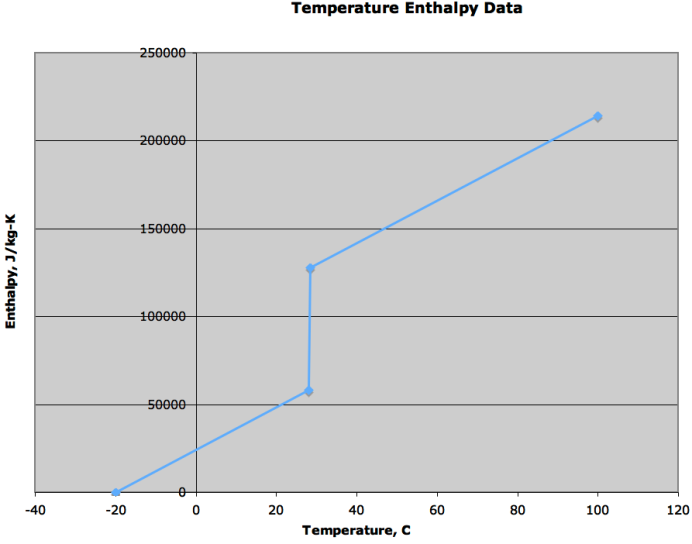
\includegraphics[width=0.9\textwidth, height=0.9\textheight, keepaspectratio=true]{media/image024.png}
\caption{Temp-Enth Example \protect \label{fig:temp-enth-example}}
\end{figure}

\paragraph{Field: Temperature x}\label{field-temperature-x}

This field is used to specify the temperature of the temperature-enthalpy function for the basic material. Units are in degree Celsius.

\paragraph{Field: Enthalpy x}\label{field-enthalpy-x}

This field specifies the enthalpy that corresponds to the previous temperature of the temperature-enthalpy function. Units are J/kg.

And, an IDF example showing how it is used in conjunction with the Material:

Note, the following Heat Balance Algorithm is necessary (only specified once). Also, when using ConductionFiniteDifference, it is more efficient to set the zone timestep shorter than those used for the ConductionTransferFunction solution algorithm. It should be set to 12 timesteps per hour or greater, and can range up to 60.

\begin{lstlisting}

HeatBalanceAlgorithm,
  ConductionFiniteDifference;


  Timestep,
  12;


  Material,
      E1 - 3 / 4 IN PLASTER OR GYP BOARD,  !- Name
      Smooth,                  !- Roughness
      1.9050000E-02,           !- Thickness {m}
      0.7264224,               !- Conductivity {W/m-K}
      1601.846,                !- Density {kg/m3}
      836.8000,                !- Specific Heat {J/kg-K}
      0.9000000,               !- Thermal Absorptance
      0.9200000,               !- Solar Absorptance
      0.9200000;               !- Visible Absorptance


  MaterialProperty:PhaseChange,
      E1 - 3 / 4 IN PLASTER OR GYP BOARD,  !- Name
      0.0,             !- Temperature coefficient,thermal conductivity(W/m K2)
      -20.,            !- Temperature 1, C
      0.01,            !- Enthalpy 1 at –20C, (J/kg)
      20.,             !- Temperature 2, C
      33400,           !- Enthalpy 2, (J/kg)
      20.5,            !- temperature 3, C
      70000,           !- Enthalpy 3, (J/kg)
      100.,            !- Temperature 4, C
      137000;          !- Enthalpy 4, (J/kg)
\end{lstlisting}

\subsection{MaterialProperty:PhaseChangeHysteresis}\label{materialpropertyphasechangehysteresis}

This object is used to describe an advanced level of physics belonging to phase change materials used in building envelopes. The base phase change input object describes a single process curve whereby a material moves from a crystallized to liquid state and back. This input object adds a hysteresis effect, allowing the melting/freezing process to follow different curves, representing an effect that is commonly seen in actual building envelope phase change material applications.

This object also allows users to enter characteristic properties of the processes instead of a detailed temperature/enthalpy curve, making it more amenable for studies in which the user does not have the detailed test data required to generate the temperature/enthalpy curve. For more information on the use of phase change materials (PCM) with hysteresis, see the Conduction Finite Difference Solution Algorithm section of the EnergyPlus Engineering Reference document.

\subsubsection{Inputs}\label{materialpropertyphasechangehysteresis-inputs}

The \hyperref[materialpropertyphasechangehysteresis]{MaterialProperty:PhaseChangeHysteresis} object includes the following inputs. For the characteristic curve properties, see the engineering reference.

\paragraph{Field: Name}\label{materialpropertyphasechangehysteresis-name}

This input must match the name of a material defined elsewhere within EnergyPlus. The thermal properties of that material are then overridden by the properties defined in this object.

\paragraph{Field: Latent Heat during the Entire Phase Change Process}\label{materialpropertyphasechangehysteresis-inputs-latent-heat-during-the-entire-phase-change-process}

This is the total amount of latent heat absorbed or discharged during the transition from solid to liquid or back, in Joules. The shapes of the enthalpy curves differ based on direction, but the total amount of energy from one state to the other does not.

\paragraph{Field: Liquid State Thermal Conductivity}\label{materialpropertyphasechangehysteresis-inputs-liquidk}

This is the constant thermal conductivity used while the material is fully liquid, in W/m-K.

\paragraph{Field: Liquid State Density}\label{materialpropertyphasechangehysteresis-inputs-liquidrho}

This is the constant density while the material is fully liquid, in kg/m3.

\paragraph{Field: Liquid State Specific Heat}\label{materialpropertyphasechangehysteresis-inputs-liquid-state-specific-heat}

This is the constant specific heat while the material is fully liquid, in J/kg-K.

\paragraph{Field: High Temperature Difference of Melting Curve}\label{materialpropertyphasechangehysteresis-inputs-high-temperature-difference-of-melting-curve}

This is the width of the enthalpy/specific heat melting curve, on the high side of the peak melting temperature, in degree Celsius (technically it is ``change in Celsius'').

\paragraph{Field: Peak Melting Temperature}\label{materialpropertyphasechangehysteresis-inputs-peak-melting-temperature}

This is the center (peak) of the melting curve, in Celsius.

\paragraph{Field: Low Temperature Difference of Melting Curve}\label{materialpropertyphasechangehysteresis-inputs-low-temperature-difference-of-melting-curve}

This is the width of the enthalpy/specific heat melting curve, on the low side of the peak melting temperature, in Celsius (technically it is ``change in Celsius'').

\paragraph{Field: Solid State Thermal Conductivity}\label{materialpropertyphasechangehysteresis-inputs-solidk}

This is the constant thermal conductivity used while the material is fully solid, in W/m-K.

\paragraph{Field: Solid State Density}\label{materialpropertyphasechangehysteresis-inputs-solidrho}

This is the constant density while the material is fully solid, in kg/m3.

\paragraph{Field: Solid State Specific Heat}\label{materialpropertyphasechangehysteresis-inputs-solid-state-specific-heat}

This is the constant specific heat while the material is fully crystallized, in J/kg-K.

\paragraph{Field: High Temperature Difference of Freezing Curve}\label{materialpropertyphasechangehysteresis-inputs-high-temperature-difference-of-freezing-curve}

This is the width of the enthalpy/specific heat freezing curve, on the high side of the peak freezing temperature, in Celsius (technically it is ``change in Celsius'').

\paragraph{Field: Peak Freezing Temperature}\label{materialpropertyphasechangehysteresis-inputs-peak-freezing-temperature}

This is the center (peak) of the freezing curve, in Celsius.  This will generally be lower than the peak melting temperature based on empirical data.  Note, however, that EnergyPlus does allow users to specify a peak freezing temperature that is higher than the peak melting temperature.

\paragraph{Field: Low Temperature Difference of Freezing Curve}\label{materialpropertyphasechangehysteresis-inputs-low-temperature-difference-of-freezing-curve}

This is the width of the enthalpy/specific heat freezing curve, on the low side of the peak freezing temperature, in Celsius (technically it is ``change in Celsius'').

An IDF example using hysteresis in conjunction with an actual Material definition is shown below.  This example includes the specification of the Heat Balance Algorithm and Timestep to show appropriate values for these inputs when MaterialProperty:PhaseChangeHysteresis is used.  Heat Balance Algorithm and Timestep are only specified once in a particular idf file.  Note that when using ConductionFiniteDifference, it is more efficient to set the zone timestep shorter than those used for the ConductionTransferFunction solution algorithm.  It should be set to 12 timesteps per hour or greater and can range up to 60.

\begin{lstlisting}

  HeatBalanceAlgorithm, ConductionFiniteDifference;

  Timestep, 12;

  Material,
    E1 - 3 / 4 IN PLASTER OR GYP BOARD,  !- Name
    Smooth,                  !- Roughness
    1.9050000E-02,           !- Thickness {m}
    0.7264224,               !- Conductivity {W/m-K}
    1601.846,                !- Density {kg/m3}
    836.8000,                !- Specific Heat {J/kg-K}
    0.9000000,               !- Thermal Absorptance
    0.9200000,               !- Solar Absorptance
    0.9200000;               !- Visible Absorptance

  MaterialProperty:PhaseChangeHysteresis,
    E1 - 3 / 4 IN PLASTER OR GYP BOARD,   !- Name
    10000,                   !- Latent Heat of Fusion {J/kg}
    0.5,                     !- Liquid State Thermal Conductivity {W/m-K}
    1500,                    !- Liquid State Density {kg/m3}
    2000,                    !- Liquid State Specific Heat {J/kg-K}
    1,                       !- High Temperature Difference of Melting Curve {deltaC}
    23,                      !- Peak Melting Temperature {C}
    1,                       !- Low Temperature Difference of Melting Curve {deltaC}
    0.5,                     !- Solid State Thermal Conductivity {W/m-K}
    1600,                    !- Solid State Density {kg/m3}
    2000,                    !- Solid State Specific Heat {J/kg-K}
    1,                       !- High Temperature Difference of Freezing Curve {deltaC}
    20,                      !- Peak Freezing Temperature {C}
    1;                       !- Low Temperature Difference of Freezing Curve {deltaC}

\end{lstlisting}

\subsubsection{Outputs}\label{materialpropertyphasechangehysteresis-outputs}

The \hyperref[materialpropertyphasechangehysteresis]{MaterialProperty:PhaseChangeHysteresis} object also includes the following outputs. The Conduction Finite Difference solution algorithm uses a finite difference solution technique where the surfaces are divided into a nodal arrangement. These outputs are specific to Conduction Finite Difference solution.

The following output variables are applicable to all opaque heat transfer surfaces when using Solution Algorithms ConductionFiniteDifference. Note that the ``X'' in the list and descriptions below must be replaced by a number that indicates the node at which the variables are being reported.  So, for example, to report the surface temperature for node 7, one would use ``CondFD Surface Temperature Node 7''.

\begin{itemize}
\item
  Zone,Average,CondFD Phase Change State \textless{}X\textgreater{} {[]}
\item
  Zone,Average,CondFD Phase Change Previous State \textless{}X\textgreater{} {[]}
\item
  Zone,Average,CondFD Phase Change Node Temperature \textless{}X\textgreater{} {[}C{]}
\item
  Zone,Average,CondFD Phase Change Node Conductivity \textless{}X\textgreater{} {[}W/m-K{]}
\item
  Zone,Average,CondFD Phase Change Node Specific Heat \textless{}X\textgreater{} {[}J/kg-K{]}
\end{itemize}

\paragraph{CondFD Phase Change State {[]}}\label{condfd-phase-change-state}

This outputs the current phase classification for the node.  The values for this output relate to the following phase categories:

\begin{itemize}
\item
-2 = liquid
\item
-1 = melting
\item
0 = transition
\item
1 = freezing
\item
2 = crystallized
\end{itemize}

\paragraph{CondFD Phase Change Previous State {[]}}\label{condfd-phase-change-previous-state}

This outputs the previous phase classification for the node.  The values for this output are the same as for the output CondFD Phase Change State above.

\paragraph{CondFD Phase Change Node Temperature \textless{}X\textgreater{} {[}C{]}}\label{condfd-phase-change-node-temperature-x-c}

This will output temperatures for a node in the surfaces being simulated with ConductionFiniteDifference. The nodes are numbered from outside to inside of the surface.  The full listing will appear in the RDD file.  This output is specific to surfaces that use the Conduction Finite Difference solution technique and have a \hyperref[materialpropertyphasechangehysteresis]{MaterialProperty:PhaseChangeHysteresis} object in the input file.  The units for this output field are degrees Celsius.

\paragraph{CondFD Phase Change Node Conductivity \textless{}X\textgreater{} {[}W/m-K{]}}\label{condfd-phase-change-node-conductivity-x-w-m-k}

This will output the conductivity for a node in the surfaces being simulated with ConductionFiniteDifference.  The nodes are numbered from outside to inside of the surface. The full listing will appear in the RDD file.  This output is specific to surfaces that use the Conduction Finite Difference solution technique and have a \hyperref[materialpropertyphasechangehysteresis]{MaterialProperty:PhaseChangeHysteresis} object in the input file.  The units for this output field are W/m-K.

\paragraph{CondFD Phase Change Node Specific Heat \textless{}X\textgreater{} {[}J/kg-K{]}}\label{condfd-phase-change-node-specific-heat-x-j-kg-k}

This will output the specific heat for a node in the surfaces being simulated with ConductionFiniteDifference.  The nodes are numbered from outside to inside of the surface. The full listing will appear in the RDD file.  This output is specific to surfaces that use the Conduction Finite Difference solution technique and have a \hyperref[materialpropertyphasechangehysteresis]{MaterialProperty:PhaseChangeHysteresis} object in the input file. The units for this output field are J/kg-K.

\subsection{MaterialProperty:VariableThermalConductivity}\label{materialpropertyvariablethermalconductivity}

This object is used to describe the temperature dependent material properties that are used in the CondFD (Conduction Finite Difference) solution algorithm. This conduction model is used when the appropriate CondFD materials are specified and the Solution Algorithm parameter is set to condFD.

\subsubsection{Inputs}\label{inputs-6-027}

\paragraph{Field: Name}\label{field-name-6-022}

This field is a regular material name specifying the material with which this additional temperature dependent property information will be associated.

\paragraph{Field Set: Temperature-Thermal Conductivity}\label{field-set-temperature-thermal-conductivity}

The temperature -- conductivity set of inputs specify a two column tabular temperature-thermal conductivity function for the basic material. Ten pairs can be specified. Specify only the number of pairs necessary. Temperature values should be strictly increasing.

\paragraph{Field: Temperature x}\label{field-temperature-x-1}

This field is used to specify the temperature of the temperature-conductivity function for the basic material. Units are C.

\paragraph{Field: Thermal Conductivity x}\label{field-thermal-conductivity-x}

This field specifies the conductivity that corresponds to the temperature (previous field) of the temperature-conductivity function. Units are W/m-K.

And, an IDF example showing how it is used in conjunction with the Materials:

Note, the following Heat Balance Algorithm is necessary (only specified once). Also, when using Conduction Finite Difference, it is more efficient to set the zone time step shorter than those used for the Conduction Transfer Function solution algorithm. It should be set to 12 time steps per hour or greater, and can range up to 60.

\begin{lstlisting}

HeatBalanceAlgorithm,
  ConductionFiniteDifference;


  Timestep,
  12;


  Material,
      PCMPlasterBoard ,      !- Name
      Smooth,                  !- Roughness
      1.9050000E-02,           !- Thickness {m}
      4.2,                     !- Conductivity {W/m-K}
      1601.846,                !- Density {kg/m3}
      836.8000,                !- Specific Heat {J/kg-K}
      0.9000000,               !- Thermal Absorptance
      0.9200000,               !- Solar Absorptance
      0.9200000;               !- Visible Absorptance


  MaterialProperty:VariableThermalConductivity,
      PCMPlasterBoard,         !- Name
      0,                       !- Temperature 1 {C}
      4.2,                     !- Thermal Conductivity 1 {W/m-K}
      22,                      !- Temperature 2 {C}
      4.2,                     !- Thermal Conductivity 2 {W/m-K}
      22.1,                    !- Temperature 3 {C}
      2.5,                     !- Thermal Conductivity 3 {W/m-K}
      100,                     !- Temperature 4 {C}
      2.5;                     !- Thermal Conductivity 4 {W/m-K}
\end{lstlisting}

\subsubsection{Outputs}\label{outputs-1-026}

The Conduction Finite Difference solution algorithm uses a finite difference solution technique where the surfaces are divided into a nodal arrangement. These outputs are specific to Conduction Finite Difference solution.

The following output variables are applicable to all opaque heat transfer surfaces when using Solution Algorithms ConductionFiniteDifference.  Note that the ``X'' in the list and descriptions below must be replaced by a number that indicates the Node at which the variables are being reported.  So, for example, to report the surface temperature for node 7, one would use ``CondFD Surface Temperature Node 7''.

\begin{itemize}
\item
  Zone,Sum,CondFD Inner Solver Loop Iteration Count {[]}
\item
  Zone,Average,CondFD Surface Temperature Node \textless{}X\textgreater{} {[}C{]}
\item
  Zone,Average,CondFD Surface Heat Flux Node \textless{}X\textgreater{} {[}W/m2{]}
\item
  Zone,Average,CondFD Surface Heat Capacitance Outer Half Node \textless{}X\textgreater{} {[}W/m2-K{]}
\item
  Zone,Average,CondFD Surface Heat Capacitance Inner Half Node \textless{}X\textgreater{} {[}W/m2-K{]}
\end{itemize}

\paragraph{CondFD Inner Solver Loop Iteration Count {[]}}\label{condfd-inner-solver-loop-iteration-count}

This outputs the count of iterations on the inner solver loop of CondFD for each surface.

\paragraph{CondFD Surface Temperature Node \textless{}X\textgreater{} {[}C{]}}\label{condfd-surface-temperature-node-x-c}

This will output temperatures for a node in the surfaces being simulated with ConductionFiniteDifference. The key values for this output variable are the surface name. The nodes are numbered from outside to inside of the surface. The full listing will appear in the RDD file.

\paragraph{CondFD Surface Heat Flux Node \textless{}X\textgreater{} {[}W/m2{]}}\label{condfd-surface-heat-flux-node-x-wm2}

This will output heat flux at each node in surfaces being simulated with ConductionFiniteDifference. The key values for this output variable are the surface name. The nodes are numbered from outside to inside of the surface. The full listing will appear in the RDD file. A positive value indicates heat flowing towards the inside face of the surface. Note that this matches the sign convention for Surface Inside Face Conduction Heat Transfer Rate per Area and is opposite the sign of Surface Outside Face Conduction Heat Transfer Rate per Area.

\paragraph{CondFD Surface Heat Capacitance Outer Half Node \textless{}X\textgreater{} {[}W/m2-K{]}}\label{condfd-surface-heat-capacitance-outer-half-node-x-wm2-k}

\paragraph{CondFD Surface Heat Capacitance Inner Half Node \textless{}X\textgreater{} {[}W/m2-K{]}}\label{condfd-surface-heat-capacitance-inner-half-node-x-wm2-k}

These will output the half-node heat capacitance in surfaces being simulated with ConductionFiniteDifference. The key values for this output variable are the surface name. The nodes are numbered from outside to inside of the surface. The full listing will appear in the RDD file. For this output, the heat capacitance is defined as the product of specific heat, density, and node thickness. Zero is reported for R-layer half-nodes and for undefined half-nodes. There is no outer half-node for Node 1 which is the outside face of the surface, and there is no inner half-node for Node N which is the inside face of the surface. CondFD Surface Heat Capacitance is only available when the user includes a Output:Diagnostics, DisplayAdvancedReportVariables designation in the input file.

\subsection{MaterialProperty:HeatAndMoistureTransfer:Settings}\label{materialpropertyheatandmoisturetransfersettings}

\textbf{Advanced/Research Usage:} This object is used to describe two of the seven additional material properties needed for the CombinedHeatAndMoistureFiniteElement heat balance solution algorithm. The settings object is used when the solutions algorithm is set to CombinedHeatAndMoistureFiniteElement and the appropriate material properties are assigned to each material. This permits the simulation of the moisture dependent thermal properties of the material as well as the transfer of moisture through, into and out of the material into the zone or exterior.

In addition to the Porosity and Initial Water content properties described here, five additional properties, described by tabulated relationships between variables, are required. These properties are;

\begin{itemize}
\item
  \hyperref[materialpropertyheatandmoisturetransfersorptionisotherm]{MaterialProperty:HeatAndMoistureTransfer:SorptionIsotherm}
\item
  \hyperref[materialpropertyheatandmoisturetransfersuction]{MaterialProperty:HeatAndMoistureTransfer:Suction}
\item
  \hyperref[materialpropertyheatandmoisturetransferredistribution]{MaterialProperty:HeatAndMoistureTransfer:Redistribution}
\item
  \hyperref[materialpropertyheatandmoisturetransferdiffusion]{MaterialProperty:HeatAndMoistureTransfer:Diffusion}
\item
  \hyperref[materialpropertyheatandmoisturetransferthermalconductivity]{MaterialProperty:HeatAndMoistureTransfer:ThermalConductivity}
\end{itemize}

All materials in a construction are required to have all material properties defined for HAMT to work.

Within the MaterialProperty:HeatAndMoistureTransfer:Settings object the following fields are defined.

\subsubsection{Inputs}\label{inputs-7-026}

\paragraph{Field: Material Name}\label{field-material-name-000}

This field is a unique reference name that the user assigns to a particular material. This name can then be referred to by other input data.

\paragraph{Field: Porosity}\label{field-porosity}

The porosity of a material is the maximum fraction, by volume, of a material that can be taken up with water. The units are {[}m3/m3{]}.

\paragraph{Field: Initial Water Content Ratio}\label{field-initial-water-content-ratio}

For this solution algorithm, the initial water content is assumed to be distributed evenly through the depth of the material. The units are {[}kg/kg{]}.

Below is an example input for the porosity and initial water content of a material.

\begin{lstlisting}

MaterialProperty:HeatAndMoistureTransfer:Settings,
        Concrete,     !- Name
        0.76,     !- Porosity
        0.2;     !- Initial (or typical) Water content
\end{lstlisting}

\subsection{MaterialProperty:HeatAndMoistureTransfer:SorptionIsotherm}\label{materialpropertyheatandmoisturetransfersorptionisotherm}

\textbf{Advanced/Research Usage:} This material property is used in conjunction with the CombinedHeatAndMoistureFiniteElement heat balance solution algorithm.

The Isotherm data relates the moisture, or water content {[}kg/m3{]} of a material with the relative humidity (RH). The water content is expected to increase as relative humidity increases, starting at zero content at 0.0 relative humidity fraction and reaching a maximum, defined by the porosity, at 1.0 relative humidity fraction, which corresponds to 100\% relative humidity. Relative humidities are entered as fraction for this object ranging from 0.0 to 1.0. These two extremes (0.0 and 1.0) are automatically set by the HAMT solution. However, if they are entered they will be used as extra data points. Data should be provided with increasing RH and moisture content up to as high an RH as possible to provide a stable solution. One possible reason for the following error message may be that a material has a very rapid increase in water content for a small change in RH, which can happen if the last entered water content point is at a low RH and the material has a very high porosity.

\begin{lstlisting}
  ** Warning ** HeatAndMoistureTransfer: Large Latent Heat for Surface ROOF
\end{lstlisting}

Another potential reason for this error being generated is the use of inappropriate values for Vapor Transfer Coefficients. See the \hyperref[surfacepropertiesvaporcoefficients]{SurfaceProperties:VaporCoefficients} object in the Advanced Surface Concepts group.

\subsubsection{Inputs}\label{inputs-8-024}

\paragraph{Field: Material Name}\label{field-material-name-1}

This field is a unique reference name that the user assigns to a particular material. This name can then be referred to by other input data.

\paragraph{Field: Number of data ~Coordinates}\label{field-number-of-data-coordinates}

A maximum of 25 coordinates can be specified.

\paragraph{Field Set: Relative Humidity-Moisture Content}\label{field-set-relative-humidity-moisture-content}

\paragraph{Field: Relative Humidity Fraction x}\label{field-relative-humidity-fraction-x}

The relative humidity of the x\(^{th}\) coordinate. The relative humidity is entered as fraction, not in percent.

\paragraph{Field: Moisture Content x}\label{field-moisture-content-x}

The Moisture Content of the x\(^{th}\) coordinate. The units are {[}kg/m3{]}

Below is an example input for a material isotherm

\begin{lstlisting}

MaterialProperty:HeatAndMoistureTransfer:SorptionIsotherm,
        Concrete,     !- Name
        10,     !- Number of data Coordinates
        0.2205,    !- Relative Humidity fraction #1
        22.31,     !- Moisture content #1
        0.202,     !- Relative Humidity fraction #2
        19.665,    !- Moisture content #2
        0.449,     !- Relative Humidity fraction #3
        40.02,     !- Moisture content #3
        0.454,     !- Relative Humidity fraction #4
        36.915,    !- Moisture content #4
        0.6506,    !- Relative Humidity fraction #5
        56.005,    !- Moisture content #5
        0.655,     !- Relative Humidity fraction #6
        52.325,    !- Moisture content #6
        0.824,     !- Relative Humidity fraction #7
        72.565,    !- Moisture content #7
        0.8725,    !- Relative Humidity fraction #8
        85.1,      !- Moisture content #8
        0.924,     !- Relative Humidity fraction #9
        91.08,     !- Moisture content #9
        0.964,     !- Relative Humidity fraction #10
        100.28;    !- Moisture content #10
\end{lstlisting}

\subsection{MaterialProperty:HeatAndMoistureTransfer:Suction}\label{materialpropertyheatandmoisturetransfersuction}

\textbf{Advanced/Research Usage:}This material property is used in conjunction with the CombinedHeatAndMoistureFiniteElement heat balance solution algorithm.

The suction data relates the liquid transport coefficient, under suction, to the water content of a material. A data point at zero water content is required. The liquid transport coefficient at the highest entered water content value is used for all liquid transport coefficient values above this water content. These coefficients are used by HAMT when the rain flag is set in the weather file.

\subsubsection{Inputs}\label{inputs-9-022}

\paragraph{Field: Material Name}\label{field-material-name-2}

This field is a unique reference name that the user assigns to a particular material. This name can then be referred to by other input data.

\paragraph{Field: Number of Suction points}\label{field-number-of-suction-points}

A maximum of 25 points can be specified.

\paragraph{Field Set: Moisture Content-Liquid Transport Coefficient}\label{field-set-moisture-content-liquid-transport-coefficient}

\paragraph{Field: Moisture Content x}\label{field-moisture-content-x-1}

The moisture content of the x\(^{th}\) point. The units are {[}kg/m3{]}.

\paragraph{Field: Liquid Transport Coefficient x}\label{field-liquid-transport-coefficient-x}

The Liquid Transport Coefficient of the x\(^{th}\) point. The units are {[}m2/s{]}.

Below is an example input for a material liquid transport coefficient under suction.

\begin{lstlisting}

MaterialProperty:HeatAndMoistureTransfer:Suction,
        Concrete,     !- Name
        5,     !- Number of Suction points
        0,     !- Moisture content 1
        0,     !- Liquid Transport Coefficient 1
        72,     !- Moisture content 2
        0.0000000000741,     !- Liquid Transport Coefficient 2
        85,     !- Moisture content 3
        0.000000000253,     !- Liquid Transport Coefficient 3
        100,     !- Moisture content 4
        0.00000000101,     !- Liquid Transport Coefficient 4
        118,     !- Moisture content 5
        0.00000000128;     !- Liquid Transport Coefficient 5
\end{lstlisting}

\subsection{MaterialProperty:HeatAndMoistureTransfer:Redistribution}\label{materialpropertyheatandmoisturetransferredistribution}

\textbf{Advanced/Research Usage:}This material property is used in conjunction with the CombinedHeatAndMoistureFiniteElement heat balance solution algorithm.

The redistribution data relates the liquid transport coefficient to the water content of a material under normal conditions. A data point at zero water content is required. The liquid transport coefficient at the highest entered water content value is used for all liquid transport coefficient values above this water content. These coefficients are used by the Heat and Moisture Transfer algorithm when the rain flag is NOT set in the weather file.

\subsubsection{Inputs}\label{inputs-10-020}

\paragraph{Field: Material Name}\label{field-material-name-3}

This field is a unique reference name that the user assigns to a particular material. This name can then be referred to by other input data.

\paragraph{Field: Number of Redistribution points}\label{field-number-of-redistribution-points}

A maximum of 25 points can be specified.

\paragraph{Field Set: Moisture Content--Liquid Transport Coefficient}\label{field-set-moisture-content-liquid-transport-coefficient-1}

\paragraph{Field: Moisture Content x}\label{field-moisture-content-x-2}

The moisture content of the x\(^{th}\) point. The units are {[}kg/m3{]}.

\paragraph{Field: Liquid Transport Coefficient x}\label{field-liquid-transport-coefficient-x-1}

The Liquid Transport Coefficient of the x\(^{th}\) point. The units are {[}m2/s{]}.

Below is an example input for the object.

\begin{lstlisting}

MaterialProperty:HeatAndMoistureTransfer:Redistribution,
        Concrete,     !- Name
        5,     !- Number of Redistribution points
        0,     !- Moisture content 1
        0,     !- Liquid Transport Coefficient 1
        72,     !- Moisture content 2
        0.00000000000741,     !- Liquid Transport Coefficient 2
        85,     !- Moisture content 3
        0.0000000000253,     !- Liquid Transport Coefficient 3
        100,     !- Moisture content 4
        0.000000000101,     !- Liquid Transport Coefficient 4
        118,     !- Moisture content 5
        0.000000000128;     !- Liquid Transport Coefficient 5
\end{lstlisting}

\subsection{MaterialProperty:HeatAndMoistureTransfer:Diffusion}\label{materialpropertyheatandmoisturetransferdiffusion}

\textbf{Advanced/Research Usage:}This material property is used in conjunction with the CombinedHeatAndMoistureFiniteElement heat balance solution algorithm.

The MU data relates the vapor diffusion resistance factor (dimensionless) to the relative humidity as fraction(RH). A data point at zero RH is required. The vapor diffusion resistance factor at the highest entered relative humidity (RH) value is used for all vapor diffusion resistance factor values above this RH.~ The relative humidity maximum value in fraction is 1.0.

\subsubsection{Inputs}\label{inputs-11-019}

\paragraph{Field: Material Name}\label{field-material-name-4}

This field is a unique reference name that the user assigns to a particular material. This name can then be referred to by other input data.

\paragraph{Field: Number of Data Pairs}\label{field-number-of-data-pairs}

A maximum of 25 pairs can be specified.

\paragraph{Field Set: Relative Humidity-Vapor Diffusion Resistance Factor}\label{field-set-relative-humidity-vapor-diffusion-resistance-factor}

\paragraph{Field: Relative Humidity Fraction \#x}\label{field-relative-humidity-fraction-x-1}

The moisture content of the x\(^{th}\) pair. The relative humidity is entered as fraction, not in percent.

\paragraph{Field: Vapor Diffusion Resistance Factor \#x}\label{field-vapor-diffusion-resistance-factor-x}

The Liquid Transport Coefficient of the x\(^{th}\) pair.

Below are some examples of the values for materials.

\begin{lstlisting}

MaterialProperty:HeatAndMoistureTransfer:Diffusion,
        Plywood,     !- Name
        3,     !- Number of data Points
        0,     !- Relative Humidity Fraction 1
        700,     !- Water Vapor Diffusion Resistance Factor 1
        0.5,     !- Relative Humidity Fraction 2
        200,     !- Water Vapor Diffusion Resistance Factor 2
        1,     !- Relative Humidity Fraction 3
        20;     !- Water Vapor Diffusion Resistance Factor 3

  MaterialProperty:HeatAndMoistureTransfer:Diffusion,
        Concrete,     !- Name
        1,     !- Number of Mu Points
        0,     !- Relative Humidity Fraction 1
        180;     !- Water Vapor Diffusion Resistance Factor 1
\end{lstlisting}

\subsection{MaterialProperty:HeatAndMoistureTransfer:ThermalConductivity}\label{materialpropertyheatandmoisturetransferthermalconductivity}

\textbf{Advanced/Research Usage:}This material property is used in conjunction with the CombinedHeatAndMoistureFiniteElement heat balance solution algorithm.

The thermal data relates the thermal conductivity {[}W/m-K{]} of a material to the moisture or water content {[}kg/m3{]}. A data point at zero water content is required. The thermal conductivity at the highest entered water content value is used for all thermal conductivity values above this water content. If this object is not defined for a material then the algorithm will use a constant value entered in the Material object for all water contents.

\subsubsection{Inputs}\label{inputs-12-018}

\paragraph{Field: Material Name}\label{field-material-name-5}

This field is a unique reference name that the user assigns to a particular material. This name can then be referred to by other input data.

\paragraph{Field: Number of Thermal Coordinates}\label{field-number-of-thermal-coordinates}

A maximum of 25 coordinates can be specified.

\paragraph{Field Set: Moisture Content- Thermal Conductivity}\label{field-set-moisture-content--thermal-conductivity}

\paragraph{Field: Moisture Content x}\label{field-moisture-content-x-3}

The moisture content of the x\(^{th}\) coordinate. The units are {[}kg/m3{]}

\paragraph{Field: Thermal Conductivity x}\label{field-thermal-conductivity-x-1}

The Thermal Conductivity of the x\(^{th}\) coordinate. The units are {[}W/m-K{]}

Below is an example of values for a material.

\begin{lstlisting}

MaterialProperty:HeatAndMoistureTransfer:ThermalConductivity
        Concrete,     !- Name
        2,     !- Number of Thermal Coordinates
        0,     !- Moisture content \#1
        1.6,     !- Thermal Conductivity \#1
        180,     !- Moisture content \#2
        2.602;     !- Thermal Conductivity \#2
\end{lstlisting}

\subsubsection{Surface Outputs}\label{surface-outputs}

\begin{itemize}
\item
  Zone,Average,HAMT Surface Average Water Content Ratio {[}kg/kg{]}
\item
  Zone,Average,HAMT Surface Inside Face Temperature {[}C{]}
\item
  Zone,Average,HAMT Surface Inside Face Relative Humidity {[}\%{]}
\item
  Zone,Average,HAMT Surface Inside Face Vapor Pressure {[}Pa{]}
\item
  Zone,Average,HAMT Surface Outside Face Temperature {[}C{]}
\item
  Zone,Average,HAMT Surface Outside Face Relative Humidity {[}\%{]}
\end{itemize}

\paragraph{HAMT Surface Average Water Content Ratio {[}kg/kg{]}}\label{hamt-surface-average-water-content-ratio-kgkg}

This output is the summed water content {[}kg/kg{]} of all cells in a surface expressed as a fraction of the mass of the water to the material mass.

\paragraph{HAMT Surface Inside Face Temperature {[}C{]}}\label{hamt-surface-inside-face-temperature-c}

This output is the temperature {[}C{]} on the internal ``surface'' of the surface.

\paragraph{HAMT Surface Inside Face Relative Humidity {[}\%{]}}\label{hamt-surface-inside-face-relative-humidity}

\paragraph{HAMT Surface Inside Face Relative Humidity {[}\%{]}}\label{hamt-surface-inside-face-relative-humidity-1}

This output is the relative humidity on the internal ``surface'' of the surface expressed as a percentage.

\paragraph{HAMT Surface Inside Face Vapor Pressure {[}Pa{]}}\label{hamt-surface-inside-face-vapor-pressure-pa}

This output is the vapor pressure {[}Pa{]} on the internal ``surface'' of the surface.

\paragraph{HAMT Surface Outside Face Temperature {[}C{]}}\label{hamt-surface-outside-face-temperature-c}

This output is the temperature on the external ``surface'' of the surface.

\paragraph{HAMT Surface Outside Face Relative Humidity {[}\%{]}}\label{hamt-surface-outside-face-relative-humidity}

This output is the relative humidity on the external ``surface'' of the surface.

\subsubsection{Internal Cell Outputs}\label{internal-cell-outputs}

Detailed profile data for the variables Temperature {[}C{]}, Relative Humidity {[}\%{]} and Water Content {[}kg/kg{]} within each surface can also be reported. To calculate the heat and moisture transfer through surfaces HAMT splits up surfaces into discrete cells. Each cell is composed of a single material and has a position within the surface. HAMT automatically assigns cells to construction objects so that there are more cells closer to boundaries between materials and also at the ``surfaces'' of the surface. It is not possible for users to define their own cells.

Each surface is made from a particular construction. The construction-surface relationship is output by HAMT to the eplusout.eio file with the following format. The output also contains the HAMT cell origins and cell number for each surface combination. The coordinate system origin is defined as the exterior surface of the construction.

\begin{lstlisting}
! <HAMT cells>, Surface Name, Construction Name, Cell Numbers
! <HAMT origins>, Surface Name, Construction Name, Cell origins (m)
HAMT cells, FLOOR,FLOOR,   1,   2,   3,   4,   5,   6,   7,   8,   9,  10,  11,  12,  13,  14,  15,  16,  17
HAMT origins,FLOOR,FLOOR, 0.0000000, 0.0122726, 0.0601616, 0.1512518, 0.2766268, 0.4240140, 0.5789860, 0.7263732, 0.8517482, 0.9428384, 0.9907274, 1.0035729, 1.0056459, 1.0090000, 1.0123541, 1.0144271, 1.0150000
\end{lstlisting}

Users can select any one of the Temperature, Relative Humidity or Water Content variables for any cell to be reported, using the following naming scheme for the output variable.

\begin{itemize}
\item
  Zone,Average,HAMT Surface Temperature Cell N {[}C{]}
\item
  Zone,Average,HAMT Surface Water Content Cell N {[}kg/kg{]}
\item
  Zone,Average,HAMT Surface Relative Humidity Cell N {[}\%{]}
\end{itemize}

\paragraph{HAMT Surface Relative Humidity Cell \textless{}N\textgreater{} {[}\%{]}}\label{hamt-surface-relative-humidity-cell-n}

This is the relative humidity of the cell in the surface.

\paragraph{HAMT Surface Temperature Cell \textless{}N\textgreater{} {[}C{]}}\label{hamt-surface-temperature-cell-n-c}

This is the temperature of the cell in the surface.

\paragraph{HAMT Surface Water Content Cell \textless{}N\textgreater{} {[}kg/kg{]}}\label{hamt-surface-water-content-cell-n-kgkg}

This is the relative water content of the cell in the surface.

\subsection{Materials for Glass Windows and Doors}\label{materials-for-glass-windows-and-doors}

All the materials for glass windows and doors have the prefix ``WindowMaterial''. The following~ WindowMaterial descriptions (Glazing, Glazing:RefractionExtinctionMethod, Gas, GasMixture, Shade, Screen and Blind) apply to glass windows and doors. The property definitions described herein for Glazing, Gas and GasMixture are supported by the National Fenestration Rating Council as standard.

``Front side'' is the side of the layer opposite the zone in which the window is defined. ``Back side'' is the side closest to the zone in which the window is defined. Therefore, for exterior windows, ``front side'' is the side closest to the outdoors. For interior windows, ``front side'' is the side closest to the zone adjacent to the zone in which the window is defined.

The solar radiation transmitted by the window layers enters the zone and is a component of the zone load. The solar radiation absorbed in each solid layer (glass, shade, screen or blind) participates in the window layer heat balance calculation. The visible transmittance and reflectance properties of the window are used in the daylighting calculation.

\subsection{WindowMaterial:Glazing}\label{windowmaterialglazing}

In the following, for exterior windows, ``front side'' is the side of the glass closest to the outside air and ``back side'' is the side closest to the zone the window is defined in. For interzone windows, ``front side'' is the side closest to the zone adjacent to the zone the window is defined in and ``back side'' is the side closest to the zone the window is defined in.

\subsubsection{Inputs}\label{inputs-13-015}

\paragraph{Field: Name}\label{field-name-7-020}

The name of the glass layer. It corresponds to a layer in a window construction.

\paragraph{Field: Optical Data Type}\label{field-optical-data-type}

Valid values for this field are SpectralAverage, Spectral, SpectralAndAngle, and BSDF.

If Optical Data Type = SpectralAverage, the values you enter for solar transmittance and reflectance are assumed to be averaged over the solar spectrum, and the values you enter for visible transmittance and reflectance are assumed to be averaged over the solar spectrum and weighted by the response of~ the human eye. There is an EnergyPlus Reference Data Set for WindowMaterial:Glazing that contains spectral average properties for many different types of glass.

If Optical Data Type = Spectral, then, in the following field, you must enter the name of a spectral data set defined with the WindowGlassSpectralData object. In this case, the values of~ solar and visible transmittance and reflectance in the fields below should be blank.

If Optical Data Type = SpectralAndAngle, then, in the last 3 fields, you must enter the name of a spectral and angle data set defined with a curve or table object with two independent variables. In this case, the Window Glass Spectral Data Set Name should be blank, and the values of solar and visible transmittance and reflectance in the fields below should be blank.

If Optical Data Type = BSDF, the \hyperref[constructioncomplexfenestrationstate]{Construction:ComplexFenestrationState} object must be used to define the window construction layers. In this case, the \hyperref[constructioncomplexfenestrationstate]{Construction:ComplexFenestrationState} object contains references to the BSDF files which contain the optical properties of the Complex Fenestration layers.

\paragraph{Field: Window Glass Spectral Data Set Name}\label{field-window-glass-spectral-data-set-name}

If Optical Data Type = Spectral, this is the name of a spectral data set defined with a WindowGlassSpectralData object.

\paragraph{Field: Thickness}\label{field-thickness-1}

The surface-to-surface thickness of the glass (m).

\paragraph{Field: Solar Transmittance at Normal Incidence}\label{field-solar-transmittance-at-normal-incidence}

Transmittance at normal incidence averaged over the solar spectrum. Used only when Optical Data Type = SpectralAverage.

For uncoated glass, when alternative optical properties are available---such as thickness, solar index of refraction, and solar extinction coefficient---they can be converted to equivalent solar transmittance and reflectance values using the equations given in \textbf{``Glass Optical Properties Conversion.''}

\paragraph{Field: Front Side Solar Reflectance at Normal Incidence}\label{field-front-side-solar-reflectance-at-normal-incidence}

Front-side reflectance at normal incidence averaged over the solar spectrum. Used only when Optical Data Type = SpectralAverage.

\paragraph{Field: Back Side Solar Reflectance at Normal Incidence}\label{field-back-side-solar-reflectance-at-normal-incidence}

Back-side reflectance at normal incidence averaged over the solar spectrum. Used only when Optical Data Type = SpectralAverage.

\paragraph{Field: Visible Transmittance at Normal Incidence}\label{field-visible-transmittance-at-normal-incidence}

Transmittance at normal incidence averaged over the solar spectrum and weighted by the response of the human eye. Used only when Optical Data Type = SpectralAverage.

For uncoated glass, when alternative optical properties are available---such as thickness, visible index of refraction, and visible extinction coefficient---they can be converted to equivalent visible transmittance and reflectance values using the equations given in \textbf{``Glass Optical Properties Conversion.''}

\paragraph{Field: Front Side Visible Reflectance at Normal Incidence}\label{field-front-side-visible-reflectance-at-normal-incidence}

Front-side reflectance at normal incidence averaged over the solar spectrum and weighted by the response of the human eye. Used only when Optical Data Type = SpectralAverage.

\paragraph{Field: Back Side Visible Reflectance at Normal Incidence}\label{field-back-side-visible-reflectance-at-normal-incidence}

Back-side reflectance at normal incidence averaged over the solar spectrum and weighted by the response of the human eye. Used only when Optical Data Type = SpectralAverage.

\paragraph{Field: Infrared Transmittance at Normal Incidence}\label{field-infrared-transmittance-at-normal-incidence}

Long-wave transmittance at normal incidence.

\paragraph{Field: Front Side Infrared Hemispherical Emissivity}\label{field-front-side-infrared-hemispherical-emissivity}

Front-side long-wave emissivity.

\paragraph{Field: Back Side Infrared Hemispherical Emissivity}\label{field-back-side-infrared-hemispherical-emissivity}

Back-side long-wave emissivity.

\paragraph{Field: Conductivity}\label{field-conductivity-1}

Thermal conductivity (W/m-K).

\paragraph{Field: Dirt Correction Factor for Solar and Visible Transmittance}\label{field-dirt-correction-factor-for-solar-and-visible-transmittance}

This is a factor that corrects for the presence of dirt on the glass. The program multiplies the fields ``Solar Transmittance at Normal Incidence'' and ``Visible Transmittance at Normal Incidence'' by this factor if the material is used as the \underline{outer} glass layer of an \underline{exterior} window or glass door.\footnote{If Optical Data Type = Spectral, the program multiplies the solar and visible transmittance at each wavelength by the dirt correction factor.} If the material is used as an inner glass layer (in double glazing, for example), the dirt correction factor is not applied because inner glass layers are assumed to be clean. Using a material with dirt correction factor \textless{} 1.0 in the construction for an interior window will result in an error message.

Representative values of the dirt correction factor are shown in Table~\ref{table:dirt-correction-factors}.

\begin{longtable}[c]{@{}llll@{}}
\caption{Dirt Correction Factors \label{table:dirt-correction-factors}} \\
\toprule
Type of Location & \multicolumn{3}{c}{Angle of Glazing} \\ \cmidrule(r){2-4}
                 & Vertical & 45$^{o}$ & Horizontal \\ \midrule
\endfirsthead

\caption[]{Dirt Correction Factors} \\
\toprule
Type of Location & \multicolumn{3}{c}{Angle of Glazing} \\ \cmidrule(r){2-4}
                 & Vertical & 45$^{o}$ & Horizontal \\ \midrule
\endhead

Non-industrial & 0.9 & 0.8 & 0.7 \\
Industrial & 0.7 & 0.6 & 0.5 \\
Very Dirty & 0.6 & 0.5 & 0.4 \\
\bottomrule
{\tiny From Appendix A, ``Daylighting in Sports Halls, Report 2,'' SportScotland, Nov. 2002 (www.sportscotland.org.uk)}
\end{longtable}

The default value of the dirt correction factor is 1.0, which means the glass is clean.

It is assumed that dirt, if present, has no effect on the IR properties of the glass.

\paragraph{Field: Solar Diffusing}\label{field-solar-diffusing}

Takes values No (the default) and Yes. If No, the glass is \underline{transparent} and beam solar radiation incident on the glass is transmitted as beam radiation with no diffuse component. If Yes, the glass is \underline{translucent} and beam solar radiation incident on the glass is transmitted as hemispherically diffuse radiation with no beam component.\footnote{EnergyPlus does not model the ``partially translucent'' case in which beam solar radiation incident on the glass is transmitted as a combination of beam and diffuse.} See Figure~\ref{fig:comparison-between-transmittance-properties}. Solar Diffusing = Yes should only be used on the \emph{innermost} pane of glass in an exterior window; it does not apply to interior windows.

For both Solar Diffusing = No and Yes, beam is reflected as beam with no diffuse component (see Figure~\ref{fig:comparison-between-transmittance-properties}). Solar Diffusing cannot be used with Window Shading Control devices (except Switchable Glazing). When attempted, the window property will be set to No for Solar Diffusing. The Surface Details report will reflect the override.

If, in the Building object, Solar Distribution = FullInteriorAndExterior, use of Solar Diffusing = Yes for glass in an exterior window will change the distribution of interior solar radiation from the window. The result is that beam solar radiation that would be transmitted by a transparent window and get absorbed by particular interior surfaces will be diffused by a translucent window and be spread over more interior surfaces. This can change the time dependence of heating and cooling loads in the zone.

In a zone with Daylighting:Detailed, translucent glazing---which is often used in skylights---will provide a more uniform daylight illuminance over the zone and will avoid patches of sunlight on the floor.

\begin{figure}[hbtp] % fig 10
\centering
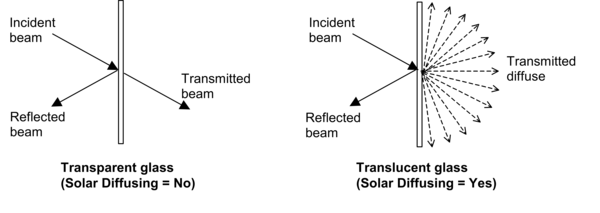
\includegraphics[width=0.9\textwidth, height=0.9\textheight, keepaspectratio=true]{media/image025.png}
\caption{Comparison between transmittance properties of transparent glass (Solar Diffusing = No) and translucent glass (Solar Diffusing = Yes). \protect \label{fig:comparison-between-transmittance-properties}}
\end{figure}

\paragraph{Field: Young's modulus}\label{field-youngs-modulus}

A measure of the stiffness of an elastic material.~ It is defined as the ratio of the uniaxial stress over the uniaxial strain in the range of stress in which Hooke's Law holds. It is used only with complex fenestration systems defined through the \hyperref[constructioncomplexfenestrationstate]{Construction:ComplexFenestrationState} object. The default value for glass is 7.2$\times$10$^{10}$ Pa.

\paragraph{Field: Poisson's ratio}\label{field-poissons-ratio}

The ratio, when a sample object is stretched, of the contraction or transverse strain (perpendicular to the applied load), to the extension or axial strain (in the direction of the applied load). This value is used only with complex fenestration systems defined through the \hyperref[constructioncomplexfenestrationstate]{Construction:ComplexFenestrationState} object. The default value for glass is 0.22.

\paragraph{Field: Window Glass Spectral and Incident Angle Transmittance Data Set Table Name}\label{field-window-glass-spectral-and-incident-angle-transmittance-data}

If Optical Data Type = SpectralAndAngle, this is the name of a spectral and angle data set of transmittance defined with a curve or table object with two independent variables. The first and second independent variables must be Angle, and Wavelength, respectively. The restriction is based on internal dataset use. Each dataset is divided into subsets for each incident angle internally.

\paragraph{Field: Window Glass Spectral and Incident Angle Front Reflectance Data Set Table Name}\label{field-window-glass-spectral-and-incident-angle-front-reflectance-data}

If Optical Data Type = SpectralAndAngle, this is the name of a spectral and angle data set of front reflectance defined with a curve or table object with two independent variables. The first and second independent variables must be Angle, and Wavelength, respectively. The restriction is based on internal dataset use. Each dataset is divided into subsets for each incident angle internally.

\paragraph{Field: Window Glass Spectral and Incident Angle Back Reflectance Data Set Table Name}\label{field-window-glass-spectral-and-incident-angle-back-reflectance-data}

If Optical Data Type = SpectralAndAngle, this is the name of a spectral and angle data set of back reflectance defined with a curve or table object with two independent variables. The first and second independent variables must be Angle, and Wavelength, respectively. The restriction is based on internal dataset use. Each dataset is divided into subsets for each incident angle internally.

It should be pointed out that when Optical Data Type = SpectralAndAngle for a glass layer in a construction, the table input data are converted into polynomial curve fits with 6 coefficients, so that all outputs of optical properties for the same construction will be curve values for a given incident angle. Therefore, the values may be slightly different from input values.

IDF examples of Spectral average and using a Spectral data set:

\begin{lstlisting}

  WindowMaterial:Glazing,
    CLEAR 3MM,       !- Name
    SpectralAverage, !- Optical Data Type
    ,                !- Window Glass Spectral Data Set Name
    0.003,           !- Thickness {m}
    0.837,           !- Solar Transmittance at Normal Incidence
    0.075,           !- Front Side Solar Reflectance at Normal Incidence
    0.075,           !- Back Side Solar Reflectance at Normal Incidence
    0.898,           !- Visible Transmittance at Normal Incidence
    0.081,           !- Front Side Visible Reflectance at Normal Incidence
    0.081,           !- Back Side Visible Reflectance at Normal Incidence
    0.0,             !- Infrared Transmittance at Normal Incidence
    0.84,            !- Front Side Infrared Hemispherical Emissivity
    0.84,            !- Back Side Infrared Hemispherical Emissivity
    0.9;             !- Conductivity {W/m-K}



  WindowMaterial:Glazing,
    SPECTRAL GLASS INNER PANE, ! Material name
    Spectral,                  ! Optical data type {SpectralAverage or Spectral}
    TestSpectralDataSet,       ! Name of spectral data set
    0.0099,                    ! Thickness {m}
    ,                          ! Solar transmittance at normal incidence
    ,                          ! Solar reflectance at normal incidence: front side
    ,                          ! Solar reflectance at normal incidence: back side
    ,                          ! Visible transmittance at normal incidence
    ,                          ! Visible reflectance at normal incidence: front side
    ,                          ! Visible reflectance at normal incidence: back side
    0.0,                       ! IR transmittance at normal incidence
    0.84,                      ! IR emissivity: front side
    0.84,                      ! IR emissivity: back side
    0.798;                     ! Conductivity {W/m-K}

\end{lstlisting}

IDF example using a SpectralAndAngle data set:

\begin{lstlisting}

  WindowMaterial:Glazing,
    SPECTRAL AND ANGLE GLASS INNER PANE, ! Material name
    SpectralAndAngle, ! Optical data type {SpectralAverage or Spectral}
    ,                 !- Name of spectral data set
    0.0099,           ! Thickness {m}
    ,                 !- Solar transmittance at normal incidence
    ,                 !- Solar reflectance at normal incidence: front side
    ,                 !- Solar reflectance at normal incidence: back side
    ,                 !- Visible transmittance at normal incidence
    ,                 !- Visible reflectance at normal incidence: front side
    ,                 !- Visible reflectance at normal incidence: back side
    0.0,              !- IR transmittance at normal incidence
    0.84,             !- IR emissivity: front side
    0.84,             !- IR emissivity: back side
    0.798,            !- Conductivity {W/m-K}
    ,                 !- Dirt Correction Factor for Solar and Visible Transmittance
    ,                 !- Solar Diffusing
    ,                 !- Young's modulus
    ,                 !- Poisson's ratio
    TranmittanceDataSet,     !- Window Glass Spectral+Incident Angle Transmittance Data Set Table Name
    FrontReflectanceDataSet, !- Window Glass Spectral+Incident Angle Front Reflectance Data Set Table Name
    BackReflectanceDataSet;  !- Window Glass Spectral+Incident Angle Back Reflectance Data Set Table Name

\end{lstlisting}

IDF example of Spectral Data Type = BSDF

\begin{lstlisting}

WindowMaterial:Glazing,
    Glass_5012_Layer,        !- Layer name : CLEAR_6.PPG
    BSDF,                    !- Optical Data Type
    ,                        !- Spectral Data name
    0.005664,                !- Thickness
    ,                        !- Solar Transmittance
    ,                        !- Solar Front Reflectance
    ,                        !- Solar Back Reflectance
    ,                        !- Visible Transmittance
    ,                        !- Visible Front Reflectance
    ,                        !- Visible Back reflectance
    0.000000,                !- IR Transmittance
    0.840000,                !-Front Emissivity
    0.840000,                !-Back Emissivity
    1.000000,                !-Conductivity
    ,                        !-Dirt Correction Factor for Sol/Vis Transmittance
    ,                        !-Solar Diffusing
    7.2e10,                  !-Young’s modulus
    0.22;                    !-Poisson’s ratio
\end{lstlisting}

\subsection{WindowMaterial:Glazing:RefractionExtinctionMethod}\label{windowmaterialglazingrefractionextinctionmethod}

This is an alternative way of specifying glass properties. Index of refraction and extinction coefficient are given instead of the transmittance and reflectance values used in \hyperref[windowmaterialglazing]{WindowMaterial:Glazing}. However, unlike \hyperref[windowmaterialglazing]{WindowMaterial:Glazing}, WindowMaterial:Glazing:RefractionExtinctionMethod is restricted to cases where the front and back optical properties of the glass are the same. This means it cannot be used for glass with a coating on one side. In that case \hyperref[windowmaterialglazing]{WindowMaterial:Glazing} should be used. Also, unlike \hyperref[windowmaterialglazing]{WindowMaterial:Glazing}, WindowMaterial:Glazing:RefractionExtinctionMethod does not allow input of glass wavelength-by-wavelength (spectral) properties.

\subsubsection{Inputs}\label{inputs-14-015}

\paragraph{Field: Name}\label{field-name-8-020}

The name of the glass layer. It corresponds to a layer in a window construction.

\paragraph{Field: Thickness}\label{field-thickness-2}

The surface-to-surface thickness of the glass (m).

\paragraph{Field: Solar Index of Refraction}\label{field-solar-index-of-refraction}

Index of refraction averaged over the solar spectrum.

\paragraph{Field: Solar Extinction Coefficient}\label{field-solar-extinction-coefficient}

Extinction coefficient averaged over the solar spectrum (m\(^{-1}\)).

\paragraph{Field: Visible Index of Refraction}\label{field-visible-index-of-refraction}

Index of refraction averaged over the solar spectrum and weighted by the response of the human eye.

\paragraph{Field: Visible Extinction Coefficient}\label{field-visible-extinction-coefficient}

Extinction coefficient averaged over the solar spectrum and weighted by the response of the human eye (m\(^{-1}\)).

\paragraph{Field: Infrared Transmittance at Normal Incidence}\label{field-infrared-transmittance-at-normal-incidence-1}

Long-wave transmittance at normal incidence.

\paragraph{Field: Infrared Hemispherical Emissivity}\label{field-infrared-hemispherical-emissivity}

Long-wave hemispherical emissivity, assumed the same on both sides of the glass.

\paragraph{Field: Conductivity}\label{field-conductivity-2}

Thermal conductivity (W/m-K).

\paragraph{Field: Dirt Correction Factor for Solar and Visible Transmittance}\label{field-dirt-correction-factor-for-solar-and-visible-transmittance-1}

This is a factor that corrects for the presence of dirt on the glass. It multiplies the solar and visible transmittance at normal Incidence (which the program calculates from the input values of thickness, solar index of refraction, solar extinction coefficient, etc.) if the material is used as the \underline{outer} glass layer of an \underline{exterior} window or glass door. If the material is used as an inner glass layer (in double glazing, for example), the dirt correction factor is not applied because inner glass layers are assumed to be clean. Using a material with dirt correction factor \textless{} 1.0 in the construction for an interior window will result in an error message.

Representative values of the direct correction factor are shown in Table~\ref{table:dirt-correction-factors}.

The default value of the dirt correction factor is 1.0, which means the glass is clean. It is assumed that dirt, if present, has no effect on the IR properties of the glass.

\paragraph{Field: Solar Diffusing}\label{field-solar-diffusing-1}

Takes values No (the default) and Yes. If No, the glass is transparent. If Yes, the glass is translucent and beam solar radiation incident on the glass is transmitted as hemispherically diffuse radiation with no beam component. (EnergyPlus does not model the ``partially translucent'' case in which beam solar radiation incident on the glass is transmitted as a combination of beam and diffuse.) Solar Diffusing = Yes should only be used on the innermost pane of glass in an exterior window; it does not apply to interior windows.

If, in the Building object, Solar Distribution = FullInteriorAndExterior, use of Solar Diffusing = Yes for glass in an exterior window will change the distribution of interior solar radiation from the window. The result is that beam solar radiation that would be transmitted by a transparent window and get absorbed by particular interior surfaces will be diffused by a translucent window and be spread over more interior surfaces. This can change the time dependence of heating and cooling loads in the zone.

In a zone with Daylighting:Detailed, translucent glazing, which is often used in skylights, will provide a more uniform daylight illuminance over the zone and will avoid patches of sunlight on the floor.

An IDF example:

\begin{lstlisting}
WindowMaterial:Glazing:RefractionExtinctionMethod,
  4MM CLEAR GLASS,  !- Material name
  0.004,            !- Thickness {m}
  1.526,            !- Solar index of refraction
  30.0 ,            !- Solar extinction coefficient (1/m)
  1.526,            !- Visible index of refraction
  30.0 ,            !- Visible extinction coefficient (1/m)
  0.0,              !- IR transmittance at normal incidence
  0.84,             !- IR emissivity
  0.9;              !- Conductivity {W/m-K}
\end{lstlisting}

\subsection{Glass Optical Properties Conversion}\label{glass-optical-properties-conversion}

\subsubsection{Conversion from Glass Optical Properties Specified as Index of Refraction and Transmittance at Normal Incidence}\label{conversion-from-glass-optical-properties-specified-as-index-of-refraction-and-transmittance-at-normal-incidence}

The optical properties of uncoated glass are sometimes specified by index of refraction, $n$, and transmittance at normal incidence, $T$.

The following equations show how to convert from this set of values to the transmittance and reflectance values required by \hyperref[windowmaterialglazing]{WindowMaterial:Glazing}. These equations apply only to \underline{uncoated} glass, and can be used to convert either spectral-average solar properties or spectral-average visible properties (in general, \(n\) and \(T\) are different for the solar and visible). Note that since the glass is uncoated, the front and back reflectances are the same and equal to the \(R\) that is solved for in the following equations.

Given \(n\) and \(T\), find \(R\):

\begin{equation*}
r = \left( \frac{n - 1}{n + 1} \right)^2
\end{equation*}

\begin{equation*}
\tau = \frac{ \left[ (1 - r)^4 + 4 r^2 T^2 \right]^{1/2} - (1 - r)^2}{2 r^2 T}
\end{equation*}

\begin{equation*}
R = r + \frac{(1 - r)^2 r \tau ^2}{1 - r^2 \tau ^2}
\end{equation*}

\textbf{Example:}

\begin{equation*}
T = 0.86156
\end{equation*}

\begin{equation*}
n = 1.526
\end{equation*}

\begin{equation*}
r = \left( \frac{1.526 - 1}{1.526 + 1} \right)^2
\end{equation*}

\begin{equation*}
\tau = 0.93974
\end{equation*}

\begin{equation*}
R = 0.07846
\end{equation*}

\subsection{WindowMaterial:GlazingGroup:Thermochromic}\label{windowmaterialglazinggroupthermochromic}

Thermochromic (TC) materials have active, reversible optical properties that vary with temperature. Thermochromic windows are adaptive window systems for incorporation into building envelopes. Thermochromic windows respond by absorbing sunlight and turning the sunlight energy into heat. As the thermochromic film warms it changes its light transmission level from less absorbing to more absorbing. The more sunlight it absorbs the lower the light level going through it. By using the suns own energy the window adapts based solely on the directness and amount of sunlight. Thermochromic materials will normally reduce optical transparency by absorption and/or reflection, and are specular (maintaining vision).

A thermochromic window is defined with a Construction object which references a special layer defined with a \hyperref[windowmaterialglazing]{WindowMaterial:Glazing}Group:Thermochromic object. The \hyperref[windowmaterialglazing]{WindowMaterial:Glazing}Group:Thermochromic object further references a series of \hyperref[windowmaterialglazing]{WindowMaterial:Glazing} objects corresponding to each specification temperature of the TC layer.

This object specifies a layer of thermochromic glass, part of a thermochromic window. An example file ThermochromicWindow.idf is included in the EnergyPlus installation.

\subsubsection{Inputs}\label{inputs-15-015}

\paragraph{Field: Name}\label{field-name-9-017}

A unique user assigned name for a particular thermochromic glass material.

\paragraph{Field Set (Optical Data Temperature, Window Material Glazing Name)}\label{field-set-optical-data-temperature-window-material-glazing-name-is-extensible.}

This object is extensible, so additional sets of the next two fields can be added to the end of this object.

\paragraph{Field:Optical Data Temperature \textless{}N\textgreater{}}\label{fieldoptical-data-temperature-n}

The temperature of the TC glass layer corresponding to the optical data of the TC layer. Unit is degree Celsius ($^\circ$C).

\paragraph{Field: Window Material Glazing Name \textless{}N\textgreater{}}\label{field-window-material-glazing-name-n}

The window glazing (defined with \hyperref[windowmaterialglazing]{WindowMaterial:Glazing}) name that provides the TC glass layer performance at the above specified temperature.

IDF Examples

\begin{lstlisting}
Construction,
  window_const,     !- Name
  Usual Glass,      !- Layer 1
  AIR 6MM,          !- Layer 2
  TCGlazings,       !- Layer 3
  AIR 6MM,          !- Layer 4
  Usual Glass;      !- Layer 5

WindowMaterial:Gas,
  AIR 6MM,          !- Name
  Air,              !- Gas Type
  0.0063;           !- Thickness {m}

! Added for thermochromic glazings
WindowMaterial:GlazingGroup:Thermochromic,
  TCGlazings,
  0 ,  TCGlazing0,
  20,  TCGlazing20,
  25,  TCGlazing25,
  30,  TCGlazing30,
  35,  TCGlazing35,
  40,  TCGlazing40,
  45,  TCGlazing45,
  50,  TCGlazing50,
  55,  TCGlazing55,
  60,  TCGlazing60,
  65,  TCGlazing65,
  75,  TCGlazing75,
  85,  TCGlazing85;

WindowMaterial:Glazing,
  TCGlazing0,       !- Name
  SpectralAverage,  !- Optical Data Type
  ,                 !- Window Glass Spectral Data Set Name
  0.0030,           !- Thickness
  0.2442,           !- Solar Transmittance at Normal Incidence
  0.7058,           !- Front Side Solar Reflectance at Normal Incidence
  0.7058,           !- Back Side Solar Reflectance at Normal Incidence
  0.3192,           !- Visible Transmittance at Normal Incidence
  0.6308,           !- Front Side Visible Reflectance at Normal Incidence
  0.6308,           !- Back Side Visible Reflectance at Normal Incidence
  0.0000,           !- Infrared Transmittance at Normal Incidence
  0.9000,           !- Front Side Infrared Hemispherical Emissivity
  0.9000,           !- Back Side Infrared Hemispherical Emissivity
  0.0199,           !- Conductivity
  1.0000,           !- Dirt Correction Factor for Solar and Visible Transmittance
  No;               !- Solar Diffusing

WindowMaterial:Glazing,
  TCGlazing20,      !- Name
  SpectralAverage,  !- Optical Data Type
  ,                 !- Window Glass Spectral Data Set Name
  0.0030,           !- Thickness
  0.2442,           !- Solar Transmittance at Normal Incidence
  0.7058,           !- Front Side Solar Reflectance at Normal Incidence
  0.7058,           !- Back Side Solar Reflectance at Normal Incidence
  0.3192,           !- Visible Transmittance at Normal Incidence
  0.6308,           !- Front Side Visible Reflectance at Normal Incidence
  0.6308,           !- Back Side Visible Reflectance at Normal Incidence
  0.0000,           !- Infrared Transmittance at Normal Incidence
  0.9000,           !- Front Side Infrared Hemispherical Emissivity
  0.9000,           !- Back Side Infrared Hemispherical Emissivity
  0.0199,           !- Conductivity
  1.0000,           !- Dirt Correction Factor for Solar and Visible Transmittance
  No;               !- Solar Diffusing

WindowMaterial:Glazing,
  TCGlazing25,      !- Name
  SpectralAverage,  !- Optical Data Type
  ,                 !- Window Glass Spectral Data Set Name
  0.0030,           !- Thickness
  0.2442,           !- Solar Transmittance at Normal Incidence
  0.7058,           !- Front Side Solar Reflectance at Normal Incidence
  0.7058,           !- Back Side Solar Reflectance at Normal Incidence
  0.3192,           !- Visible Transmittance at Normal Incidence
  0.6308,           !- Front Side Visible Reflectance at Normal Incidence
  0.6308,           !- Back Side Visible Reflectance at Normal Incidence
  0.0000,           !- Infrared Transmittance at Normal Incidence
  0.9000,           !- Front Side Infrared Hemispherical Emissivity
  0.9000,           !- Back Side Infrared Hemispherical Emissivity
  0.0199,           !- Conductivity
  1.0000,           !- Dirt Correction Factor for Solar and Visible Transmittance
  No;               !- Solar Diffusing

WindowMaterial:Glazing,
  TCGlazing30,      !- Name
  SpectralAverage,  !- Optical Data Type
  ,                 !- Window Glass Spectral Data Set Name
  0.0030,           !- Thickness
  0.2442,           !- Solar Transmittance at Normal Incidence
  0.7058,           !- Front Side Solar Reflectance at Normal Incidence
  0.7058,           !- Back Side Solar Reflectance at Normal Incidence
  0.3192,           !- Visible Transmittance at Normal Incidence
  0.6308,           !- Front Side Visible Reflectance at Normal Incidence
  0.6308,           !- Back Side Visible Reflectance at Normal Incidence
  0.0000,           !- Infrared Transmittance at Normal Incidence
  0.9000,           !- Front Side Infrared Hemispherical Emissivity
  0.9000,           !- Back Side Infrared Hemispherical Emissivity
  0.0199,           !- Conductivity
  1.0000,           !- Dirt Correction Factor for Solar and Visible Transmittance
  No;               !- Solar Diffusing

WindowMaterial:Glazing,
  TCGlazing35,      !- Name
  SpectralAverage,  !- Optical Data Type
  ,                 !- Window Glass Spectral Data Set Name
  0.0030,           !- Thickness
  0.2442,           !- Solar Transmittance at Normal Incidence
  0.7058,           !- Front Side Solar Reflectance at Normal Incidence
  0.7058,           !- Back Side Solar Reflectance at Normal Incidence
  0.3192,           !- Visible Transmittance at Normal Incidence
  0.6308,           !- Front Side Visible Reflectance at Normal Incidence
  0.6308,           !- Back Side Visible Reflectance at Normal Incidence
  0.0000,           !- Infrared Transmittance at Normal Incidence
  0.9000,           !- Front Side Infrared Hemispherical Emissivity
  0.9000,           !- Back Side Infrared Hemispherical Emissivity
  0.0199,           !- Conductivity
  1.0000,           !- Dirt Correction Factor for Solar and Visible Transmittance
  No;               !- Solar Diffusing

WindowMaterial:Glazing,
  TCGlazing40,      !- Name
  SpectralAverage,  !- Optical Data Type
  ,                 !- Window Glass Spectral Data Set Name
  0.0030,           !- Thickness
  0.2442,           !- Solar Transmittance at Normal Incidence
  0.7058,           !- Front Side Solar Reflectance at Normal Incidence
  0.7058,           !- Back Side Solar Reflectance at Normal Incidence
  0.3192,           !- Visible Transmittance at Normal Incidence
  0.6308,           !- Front Side Visible Reflectance at Normal Incidence
  0.6308,           !- Back Side Visible Reflectance at Normal Incidence
  0.0000,           !- Infrared Transmittance at Normal Incidence
  0.9000,           !- Front Side Infrared Hemispherical Emissivity
  0.9000,           !- Back Side Infrared Hemispherical Emissivity
  0.0199,           !- Conductivity
  1.0000,           !- Dirt Correction Factor for Solar and Visible Transmittance
  No;               !- Solar Diffusing

WindowMaterial:Glazing,
  TCGlazing45,      !- Name
  SpectralAverage,  !- Optical Data Type
  ,                 !- Window Glass Spectral Data Set Name
  0.0030,           !- Thickness
  0.2442,           !- Solar Transmittance at Normal Incidence
  0.7058,           !- Front Side Solar Reflectance at Normal Incidence
  0.7058,           !- Back Side Solar Reflectance at Normal Incidence
  0.3192,           !- Visible Transmittance at Normal Incidence
  0.6308,           !- Front Side Visible Reflectance at Normal Incidence
  0.6308,           !- Back Side Visible Reflectance at Normal Incidence
  0.0000,           !- Infrared Transmittance at Normal Incidence
  0.9000,           !- Front Side Infrared Hemispherical Emissivity
  0.9000,           !- Back Side Infrared Hemispherical Emissivity
  0.0199,           !- Conductivity
  1.0000,           !- Dirt Correction Factor for Solar and Visible Transmittance
  No;               !- Solar Diffusing

WindowMaterial:Glazing,
  TCGlazing50,      !- Name
  SpectralAverage,  !- Optical Data Type
  ,                 !- Window Glass Spectral Data Set Name
  0.0030,           !- Thickness
  0.2442,           !- Solar Transmittance at Normal Incidence
  0.7058,           !- Front Side Solar Reflectance at Normal Incidence
  0.7058,           !- Back Side Solar Reflectance at Normal Incidence
  0.3192,           !- Visible Transmittance at Normal Incidence
  0.6308,           !- Front Side Visible Reflectance at Normal Incidence
  0.6308,           !- Back Side Visible Reflectance at Normal Incidence
  0.0000,           !- Infrared Transmittance at Normal Incidence
  0.9000,           !- Front Side Infrared Hemispherical Emissivity
  0.9000,           !- Back Side Infrared Hemispherical Emissivity
  0.0199,           !- Conductivity
  1.0000,           !- Dirt Correction Factor for Solar and Visible Transmittance
  No;               !- Solar Diffusing

WindowMaterial:Glazing,
  TCGlazing55,      !- Name
  SpectralAverage,  !- Optical Data Type
  ,                 !- Window Glass Spectral Data Set Name
  0.0030,           !- Thickness
  0.2442,           !- Solar Transmittance at Normal Incidence
  0.7058,           !- Front Side Solar Reflectance at Normal Incidence
  0.7058,           !- Back Side Solar Reflectance at Normal Incidence
  0.3192,           !- Visible Transmittance at Normal Incidence
  0.6308,           !- Front Side Visible Reflectance at Normal Incidence
  0.6308,           !- Back Side Visible Reflectance at Normal Incidence
  0.0000,           !- Infrared Transmittance at Normal Incidence
  0.9000,           !- Front Side Infrared Hemispherical Emissivity
  0.9000,           !- Back Side Infrared Hemispherical Emissivity
  0.0199,           !- Conductivity
  1.0000,           !- Dirt Correction Factor for Solar and Visible Transmittance
  No;               !- Solar Diffusing

WindowMaterial:Glazing,
  TCGlazing60,      !- Name
  SpectralAverage,  !- Optical Data Type
  ,                 !- Window Glass Spectral Data Set Name
  0.0030,           !- Thickness
  0.2442,           !- Solar Transmittance at Normal Incidence
  0.7058,           !- Front Side Solar Reflectance at Normal Incidence
  0.7058,           !- Back Side Solar Reflectance at Normal Incidence
  0.3192,           !- Visible Transmittance at Normal Incidence
  0.6308,           !- Front Side Visible Reflectance at Normal Incidence
  0.6308,           !- Back Side Visible Reflectance at Normal Incidence
  0.0000,           !- Infrared Transmittance at Normal Incidence
  0.9000,           !- Front Side Infrared Hemispherical Emissivity
  0.9000,           !- Back Side Infrared Hemispherical Emissivity
  0.0199,           !- Conductivity
  1.0000,           !- Dirt Correction Factor for Solar and Visible Transmittance
  No;               !- Solar Diffusing

WindowMaterial:Glazing,
  TCGlazing65,      !- Name
  SpectralAverage,  !- Optical Data Type
  ,                 !- Window Glass Spectral Data Set Name
  0.0030,           !- Thickness
  0.2442,           !- Solar Transmittance at Normal Incidence
  0.7058,           !- Front Side Solar Reflectance at Normal Incidence
  0.7058,           !- Back Side Solar Reflectance at Normal Incidence
  0.3192,           !- Visible Transmittance at Normal Incidence
  0.6308,           !- Front Side Visible Reflectance at Normal Incidence
  0.6308,           !- Back Side Visible Reflectance at Normal Incidence
  0.0000,           !- Infrared Transmittance at Normal Incidence
  0.9000,           !- Front Side Infrared Hemispherical Emissivity
  0.9000,           !- Back Side Infrared Hemispherical Emissivity
  0.0199,           !- Conductivity
  1.0000,           !- Dirt Correction Factor for Solar and Visible Transmittance
  No;               !- Solar Diffusing

WindowMaterial:Glazing,
  TCGlazing75,      !- Name
  SpectralAverage,  !- Optical Data Type
  ,                 !- Window Glass Spectral Data Set Name
  0.0030,           !- Thickness
  0.2442,           !- Solar Transmittance at Normal Incidence
  0.7058,           !- Front Side Solar Reflectance at Normal Incidence
  0.7058,           !- Back Side Solar Reflectance at Normal Incidence
  0.3192,           !- Visible Transmittance at Normal Incidence
  0.6308,           !- Front Side Visible Reflectance at Normal Incidence
  0.6308,           !- Back Side Visible Reflectance at Normal Incidence
  0.0000,           !- Infrared Transmittance at Normal Incidence
  0.9000,           !- Front Side Infrared Hemispherical Emissivity
  0.9000,           !- Back Side Infrared Hemispherical Emissivity
  0.0199,           !- Conductivity
  1.0000,           !- Dirt Correction Factor for Solar and Visible Transmittance
  No;               !- Solar Diffusing

WindowMaterial:Glazing,
  TCGlazing85,      !- Name
  SpectralAverage,  !- Optical Data Type
  ,                 !- Window Glass Spectral Data Set Name
  0.0030,           !- Thickness
  0.2442,           !- Solar Transmittance at Normal Incidence
  0.7058,           !- Front Side Solar Reflectance at Normal Incidence
  0.7058,           !- Back Side Solar Reflectance at Normal Incidence
  0.3192,           !- Visible Transmittance at Normal Incidence
  0.6308,           !- Front Side Visible Reflectance at Normal Incidence
  0.6308,           !- Back Side Visible Reflectance at Normal Incidence
  0.0000,           !- Infrared Transmittance at Normal Incidence
  0.9000,           !- Front Side Infrared Hemispherical Emissivity
  0.9000,           !- Back Side Infrared Hemispherical Emissivity
  0.0199,           !- Conductivity
  1.0000,           !- Dirt Correction Factor for Solar and Visible Transmittance
  No;               !- Solar Diffusing
\end{lstlisting}

\subsubsection{Outputs}\label{outputs-3-019}

\paragraph{Surface Window Thermochromic Layer Temperature {[}C{]}}\label{surface-window-thermochromic-layer-temperature-c}

The temperature of the TC glass layer of a TC window at each time step.

\paragraph{Surface Window Thermochromic Layer Property Specification Temperature {[}C{]}}\label{surface-window-thermochromic-layer-property-specification-temperature-c}

The temperature under which the optical data of the TC glass layer are specified.

The overall properties (U-factor/SHGC/VT) of the thermochromic windows at different specification temperatures are reported in the EIO file. These window constructions are created by EnergyPlus during run time. They have similar names with suffix ``\_TC\_XX'' where XX represents a specification temperature.

\subsection{WindowMaterial:Gas}\label{windowmaterialgas}

This object specifies the properties of the gas between the panes of a multi-pane window. Gas Type = Custom allows you to specify the properties of gases other than air, Argon, Krypton or Xenon. There is an EnergyPlus Reference Data Set for Material:WindowGas that contains several types of gas of different thicknesses. See Material:WindowGasMixture for the case that the gas fill is a mixture of different gases.

\subsubsection{Inputs}\label{inputs-16-011}

\paragraph{Field: Name}\label{field-name-10-016}

The name of the gas fill. It refers to a layer in a window construction.

\paragraph{Field: Gas Type}\label{field-gas-type}

The type of gas. The choices are Air, Argon, Krypton, or Xenon. If Gas Type = Custom you can use Conductivity Coefficient A, etc. to specify the properties of a different type of gas.

\paragraph{Field: Thickness}\label{field-thickness-3}

The thickness (m) of the gas layer.

\paragraph{Properties for Custom Gas Types}\label{properties-for-custom-gas-types}

The following entries are used only if Gas Type = Custom. The A and B coefficients are those in the following expression that gives a property value as a function of temperature in degrees K:

\begin{equation}
Property = Coefficien{t_A} + Coefficien{t_B}*Temperatur{e_K} + Coefficien{t_C}*Temperature_K^2
\end{equation}

\paragraph{Field: Conductivity Coefficient A}\label{field-conductivity-coefficient-a}

The A coefficient for gas conductivity (W/m-K). Used only if Gas Type = Custom.

\paragraph{Field: Conductivity Coefficient B}\label{field-conductivity-coefficient-b}

The B coefficient for gas conductivity (W/m-K\(^{2}\)). Used only if Gas Type = Custom.

\paragraph{Field: Conductivity Coefficient C}\label{field-conductivity-coefficient-c}

The C coefficient for gas conductivity (W/m-K\(^{3}\)).~ Used only if Gas Type = Custom.

\paragraph{Field: Viscosity Coefficient A}\label{field-viscosity-coefficient-a}

The A coefficient for gas viscosity (kg/m-s). Used only if Gas Type = Custom.

\paragraph{Field: Viscosity Coefficient B}\label{field-viscosity-coefficient-b}

The B coefficient for gas viscosity (kg/m-s-K). Used only if Gas Type = Custom.

\paragraph{Field: Viscosity Coefficient C}\label{field-viscosity-coefficient-c}

The C coefficient for gas viscosity (kg/m-s-K\(^{2}\)).~ Used only if Gas Type = Custom.

\paragraph{Field: Specific Heat Coefficient A}\label{field-specific-heat-coefficient-a}

The A coefficient for gas specific heat (J/kg-K). Used only if Gas Type = Custom.

\paragraph{Field: Specific Heat Coefficient B}\label{field-specific-heat-coefficient-b}

The B coefficient for gas specific heat (J/kg-K\(^{2}\)). Used only if Gas Type = Custom.

\paragraph{Field: Specific Heat Coefficient C}\label{field-specific-heat-coefficient-c}

The C coefficient for gas specific heat (J/kg-K\(^{3}\)).~ Used only if Gas Type = Custom.

\paragraph{Field: Specific Heat Ratio}\label{field-specific-heat-ratio}

The specific heat ratio for gas.~ Used only if Gas Type = Custom.

\paragraph{Field: Molecular Weight}\label{field-molecular-weight}

The molecular weight for gas.~ The molecular weight is the mass of 1 mol of the substance.~ This has a numerical value which is the average molecular mass of the molecules in the substance multiplied by Avogadro's constant. (kg/kmol) (Shown in the IDD as g/mol for consistency)

\paragraph{Field: Specific Heat Ratio}\label{field-specific-heat-ratio-1}

The specific heat ratio for gas.~ The specific heat ratio of a gas is the ratio of the specific heat at contant pressure, to the specific heat at constant volume.~ Used only if Gas Type = Custom.

An IDF example:

\begin{lstlisting}

WindowMaterial:Gas,AIRGAP,
    AIR,      ! Gas type (Air - Argon - Krypton - Xenon - Custom)]
    0.0125;   ! Thickness {m} 1/2 inch
\end{lstlisting}

An IDF example to be used with a \hyperref[windowmaterialgap]{WindowMaterial:Gap} definition (see below)

\begin{lstlisting}

WindowMaterial:Gas,
  Gas_1_W_0_0100,                                     !- gap name - Air
  Air,                                                !- type
  0.0100;                                             !- thickness
\end{lstlisting}

An IDF example for a Custom Gas

\begin{lstlisting}

WindowMaterial:Gas,
  Gas_16_W_0_0003,                   !- gap name
  Custom,                            !- type
  0.0003,                            !- thickness
  2.873000e-003,                     !- Conductivity Coefficient A
  7.760000e-005,                     !- Conductivity Coefficient B
  0.000000e+000,                     !- Conductivity Coefficient C
  3.723000e-006,                     !- Conductivity Viscosity A
  4.940000e-008,                     !- Conductivity Viscosity B
  0.000000e+000,                     !- Conductivity Viscosity C
  1002.737000,                       !- Specific Heat Coefficient A
  0.012324,                          !- Specific Heat Coefficient B
  0.000000,                          !- Specific Heat Coefficient C
  28.969999,                         !- Molecular Weight
  1.400000;                          !- Specific Heat Ratio
\end{lstlisting}

\subsection{WindowMaterial:GasMixture}\label{windowmaterialgasmixture}

This object allows you to specify the fill between the panes of a multi-pane window to be a mixture of two, three or four different gases chosen from air, argon, krypton and xenon. It can also be used if only one type of gas in the fill. In this case you can also use \hyperref[windowmaterialgas]{WindowMaterial:Gas}. Note that the fractions of gas types in the mixture should add up to 1.0.

\subsubsection{Inputs}\label{inputs-17-009}

\paragraph{Field: Name}\label{field-name-11-014}

The name of the gas mixture. It refers to a layer in a window construction.

\paragraph{Field: Thickness}\label{field-thickness-4}

The thickness (m) of the gas mixture layer.

\paragraph{Field: Number of Gases in Mixture}\label{field-number-of-gases-in-mixture}

The number of different types of gas in the mixture ( a value from 1 to 4)

\paragraph{Set: Gas Type-Fraction (up to 4)}\label{set-gas-type-fraction-up-to-4}

\paragraph{Field: Gas 1 Type}\label{field-gas-1-type}

The type of~ the first gas in the mixture. Choices are Air, Argon, Krypton and Xenon.

\paragraph{Field: Gas 1 Fraction}\label{field-gas-1-fraction}

The fraction of the first gas in the mixture.

An IDF example:

\begin{lstlisting}

WindowMaterial:GasMixture,ArgonKryptonMix,
  0.0125,   ! Thickness {m} 1/2 inch
  2,        ! Number of Gases in Mixture
  Argon,    ! Gas 1 Type
  0.6,      ! Gas 1 Fraction
  Krypton,  ! Gas 2 Type
  0.4;      ! Gas 2 Fraction
\end{lstlisting}

\subsection{WindowMaterial:Gap}\label{windowmaterialgap}

This input object is used to define the gap between two layers in a complex fenestration system, where the \hyperref[constructioncomplexfenestrationstate]{Construction:ComplexFenestrationState} object is used. It references the gas or gas mixtures defined in the \hyperref[windowmaterialgas]{WindowMaterial:Gas} and \hyperref[windowmaterialgasmixture]{WindowMaterial:GasMixture} objects. It is referenced as a layer in the \hyperref[constructioncomplexfenestrationstate]{Construction:ComplexFenestrationState} object ;it cannot be referenced as a layer from the Construction object.

\subsubsection{Inputs}\label{inputs-18-009}

\paragraph{Field: Name}\label{field-name-12-011}

Unique name of the gap.

\paragraph{Field: Thickness}\label{field-thickness-5}

The thickness (m) of the gap layer.

\paragraph{Field: Pressure}\label{field-pressure-000}

The pressure (Pa) of the gas in the gap layer, used to calculate the gas properties of the glazing system gap. The default value is one standard atmospheric pressure (101,325 Pa). When modeling vacuum glazing, this value should represent the pressure in the evacuated glazing system. If this pressure is less that the ThermalModelParams:PressureLimit value, the the glazing system will be modeled as a vacuum glazing.

\paragraph{Field: Deflection State}\label{field-deflection-state}

This field is used when modeling the deflection of the glass layers in a window if the \hyperref[windowthermalmodelparams]{WindowThermalModel:Params} value for ``deflection model'' is ``MeasuredDeflection''.

\paragraph{Field: Support Pillar}\label{field-support-pillar}

References the support pillar of the gap layer if vacuum glazing is being modeled.~ If left empty, then it is considered that gap layer does not have support pillars.

\paragraph{Field: Gas (or GasMixture)}\label{field-gas-or-gasmixture}

References gas (\hyperref[windowmaterialgas]{WindowMaterial:Gas}) or gas mixture (\hyperref[windowmaterialgasmixture]{WindowMaterial:GasMixture}) of the gap layer.

An IDF example for simple glazing:

\begin{lstlisting}

WindowMaterial:Gas,
  Gas_1_W_0_0120,                                !- gap name - Air
  Air,                                           !- type
  0.0120;                                        !- thickness


  WindowMaterial:Gap,
  Gap_1_Layer,                                   !- gap name: Air
  0.0120,                                        !- thickness
  Gas_1_W_0_0120,                                !- Gas (or Gas Mixture) name
  101325.0000;                                   !- pressure
\end{lstlisting}

An IDF example for vacuum glazing:

\begin{lstlisting}

WindowMaterial:Gap,
  Gap_16_Layer,                     !- gap name: Vacuum_0.001_pr-0.5_ps-50.8
  0.0003,                                             !- thicknessGas_16_W_0_0003,                                    !- Gas (or Gas Mixture) name
  0.1333,                                             !- pressure
  ,                                                   !- deflection state
  SupportPillar_16_Gap_1;                             !- SupportPillar


  WindowGap:SupportPillar,
  SupportPillar_16_Gap_1,                             !- Name
  0.0508,                                             !- spacing
  0.0005;                                             !- radius
\end{lstlisting}

\subsection{WindowGap:DeflectionState}\label{windowgapdeflectionstate}

This input object is used to enter data describing deflection state of the gap.~ It is referenced from \hyperref[windowmaterialgap]{WindowMaterial:Gap} object only and it is used only when deflection model is set to MeasuredDeflection (see \hyperref[windowthermalmodelparams]{WindowThermalModel:Params}), otherwise it is ignored.

\subsubsection{Inputs}\label{inputs-19-006}

\paragraph{Field: Name}\label{field-name-13-010}

Unique name of the deflection state.

\paragraph{Field: Deflected Thickness}\label{field-deflected-thickness}

The thickness (m) of the gap in deflected state.~ It represents value of deflection at point of maximum which is usually at the center point of glazing system.~ It is used only with tarcog algorithm set to Measured Deflection (\hyperref[windowthermalmodelparams]{WindowThermalModel:Params}), otherwise this field will be ignored.

An IDF example where \hyperref[windowthermalmodelparams]{WindowThermalModel:Params} Deflection Model = MeasuredDeflection:

\begin{lstlisting}

WindowMaterial:Gap,
  Gap_1_Layer,                                  !- gap name: Air
  0.0120,                                       !- thickness
  Gas_1_W_0_0120,                               !- Gas (or Gas Mixture) name
  101325.0000,                                  !- pressure
  Gap_1_Deflection;                              !- deflection state


  WindowGap:DeflectionState,       !- deflection state of gap
    Gap_1_Deflection,              !- name
    0.011;                         !- gap thickness in deflected state
\end{lstlisting}

\subsection{WindowGap:SupportPillar}\label{windowgapsupportpillar}

This input object is used to enter data describing support pillar of the gap.~ Support pillars are used in vacuum glazing in order to prevent deflection of glass layers.

\begin{figure}[hbtp] % fig 11
\centering
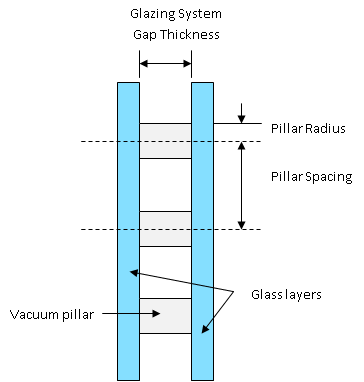
\includegraphics[width=0.9\textwidth, height=0.9\textheight, keepaspectratio=true]{media/image029.png}
\caption{Support Pillar \protect \label{fig:support-pillar}}
\end{figure}

\subsubsection{Inputs}\label{inputs-20-006}

\paragraph{Field: Name}\label{field-name-14-009}

Unique name of the support pillar.

\paragraph{Field: Spacing}\label{field-spacing}

Distance (m) between support pillar centers (see the Engineering reference document for more information).

\paragraph{Field: Radius}\label{field-radius}

The radius (m) of the support pillar (see Engineering reference document for more information).

An IDF example for vacuum glazing (see Vacuum Glazing example in \hyperref[windowmaterialgap]{WindowMaterial:Gap} above) is as follows:

\begin{lstlisting}

WindowGap:SupportPillar,       !- gap support pillar
    SupportPillar_16_Gap_1,      !- basis matrix name
    0.05,                        !- pillar spacing
    0.005;                       !- pillar radius
\end{lstlisting}

\subsection{WindowMaterial:SimpleGlazingSystem}\label{windowmaterialsimpleglazingsystem}

\warning{This model should be used with caution. There may be significant differences in performance between the simple window system and the usual more detailed model.}

This input object differs from the other WindowMaterial objects in that it describes an entire glazing system rather than individual layers. This object is used when only very limited information is available on the glazing layers or when specific performance levels are being targeted. The layer by layer description offers superior method of modeling windows that should be used instead of this object when sufficient data are available. This object accesses a model that turns simple performance indices into a fuller model of the glazing system.

The performance indices are U-factor and Solar Heat Gain Coefficient, and optionally Visible Transmittance. The values for these performance indices can be selected by the user to represent either glazing-only windows (with no frame) or an average window performance that includes the frame. Inside the program the model produces an equivalent window glazing layer with no frame. The properties of the modeled glazing layer are reported to the EIO file using the IDF input object syntax for the \hyperref[windowmaterialglazing]{WindowMaterial:Glazing} input object. This equivalent layer could be reused in subsequent models if desired, however there will be important differences in the modeled window performance because the simple glazing system model includes its own special model for angular dependence when incident beam solar is not normal to the plane of the window.

When this object is referenced in a Construction object, it cannot be used with other glazing or gas material layers. Shades or blinds cannot be located between the glass, but these can be used on the inside or the outside of the glazing system.~~ If the glazing system does have between-the-glass shades or blinds, then the U and SHGC values entered in this object should include the impacts of those layers. Adding window treatment layers such as shades or screens will alter the overall performance to be different than the performance levels prescribed in this object.

\subsubsection{Inputs}\label{inputs-21-006}

\paragraph{Field: Name}\label{field-name-15-009}

The name of the glazing system.~ This value is unique across all constructions.

\paragraph{Field: U-Factor}\label{field-u-factor}

This field describes the value for window system U-Factor, or overall heat transfer coefficient. Units are in W/m$^{2}$-K. This is the rated (NFRC) value for U-factor under winter heating conditions. The U-factor is assumed to be for vertically mounted products.

In versions up till 9.6.0, the maximum allowable input is U-7.0 W/m$^{2}$-K, and the effective upper limit of the glazing generated by the underlying model is around U-5.8 W/m$^{2}$-K. In later versions, such upper bound of the input U value is removed. So is the mismatch between the user input U and the effective U is resolved.

\paragraph{Field: Solar Heat Gain Coefficient}\label{field-solar-heat-gain-coefficient}

This field describes the value for SHGC, or solar heat gain coefficient. There are no units. This is the rated (NFRC) value for SHGC under summer cooling conditions and represents SHGC for normal incidence and vertical orientation.

\paragraph{Field: Visible Transmittance}\label{field-visible-transmittance}

This field is optional. If it is omitted, then the visible transmittance properties are taken from the solar properties. If it is included then the model includes it when developing properties for the glazing system. This is the rated (NFRC) value for visible transmittance at normal incidence.

An example of this object is as follows:

\begin{lstlisting}

WindowMaterial:SimpleGlazingSystem,
      SimpleWindow:DOUBLE PANE WINDOW , !- Name
      2.716 , !-  U-Factor
      0.763 , !-  Solar Heat Gain Coefficient
      0.812 ; !-  Visible Transmittance
\end{lstlisting}

\subsection{WindowMaterial:Shade}\label{windowmaterialshade}

This object specifies the properties of window shade materials. Reflectance and emissivity properties are assumed to be the same on both sides of the shade. Shades are considered to be perfect diffusers (all transmitted and reflected radiation is hemispherically-diffuse) with transmittance and reflectance independent of angle of incidence. There is an EnergyPlus Reference Data Set for WindowMaterial:Shade that contains properties of generic window shades.

Window shades can be on the inside of the window (``interior shades''), on the outside of the window (``exterior shades''), or between glass layers (``between-glass shades''). When in place, the shade is assumed to cover all of the glazed part of the window, including dividers; it does not cover any of the window frame, if present. The plane of the shade is assumed to be parallel to the glazing.

WindowMaterial:Shade can be used for diffusing materials such as drapery and translucent roller shades. For slat-type shading devices, like Venetian blinds, that have a strong angular dependence of transmission, absorption and reflection, it is better to use \hyperref[windowmaterialblind]{WindowMaterial:Blind}. \hyperref[windowmaterialscreen]{WindowMaterial:Screen} should be used to model wire mesh insect screens where the solar and visible transmission and reflection properties vary with the angle of incidence of solar radiation.

Transmittance and reflectance values for drapery material with different color and openness of weave can be obtained from manufacturers or determined from 2001 ASHRAE Fundamentals, Chapter 30, Fig. 31.

There are two methods of assigning a shade to a window:

\subsubsection{Inputs}\label{inputs-22-005}

\paragraph{Method 1:}\label{method-1}

\begin{itemize}

\item 1) Define the construction of the window without the shade, the so-called ``bare'' construction.
	
\item 2) Reference the bare construction in the \hyperref[fenestrationsurfacedetailed]{FenestrationSurface:Detailed} for the window.

\item 3) Define the WindowMaterial:Shade.

\item 4) Define a \hyperref[windowpropertyshadingcontrol]{WindowShadingControl} for the window in which you (a) specify that this WindowMaterial:Shade is the window's shading device and (b) specify how the shade is controlled.

\end{itemize}

\paragraph{Method 2:}\label{method-2}

\begin{itemize}

\item 1) Define the Construction of the window without the shade, the so-called ``bare'' construction.

\item 2) Reference the bare construction in the \hyperref[fenestrationsurfacedetailed]{FenestrationSurface:Detailed} for the window.

\item 3) Define the WindowMaterial:Shade.

\item 4) Define another Construction, called the ``shaded construction,'' that includes the WindowMaterial:Shade.

\item 5) Define a \hyperref[windowpropertyshadingcontrol]{WindowShadingControl} for the window in which you (a) reference the shaded construction and (b) specify how the shade is controlled.

Note that \hyperref[windowpropertyshadingcontrol]{WindowShadingControl} has to be used with either method, even if the shade is in place at all times. You will get an error message if you try to reference a shaded construction directly from \hyperref[fenestrationsurfacedetailed]{FenestrationSurface:Detailed}.

\end{itemize}

\paragraph{Field: Name}\label{field-name-16-009}

Name of the shade. It is referenced as an inside or outside layer in a window construction.

\paragraph{Field: Solar Transmittance}\label{field-solar-transmittance}

Transmittance averaged over the solar spectrum. Assumed independent of incidence angle.

\paragraph{Field: Solar Reflectance}\label{field-solar-reflectance}

Reflectance averaged over the solar spectrum. Assumed same on both sides of shade and independent of incidence angle.

\paragraph{Field: Visible Transmittance}\label{field-visible-transmittance-1}

Transmittance averaged over the solar spectrum and weighted by the response of the human eye. Assumed independent of incidence angle.

\paragraph{Field: Visible Reflectance}\label{field-visible-reflectance}

Reflectance averaged over the solar spectrum and weighted by the response of the human eye. Assumed same on both side of shade and independent of incidence angle.

\paragraph{Field: Infrared Hemispherical Emissivity}\label{field-infrared-hemispherical-emissivity-201710020805}

Effective long-wave emissivity. Assumed same on both sides of shade. We can approximate this~ effective emissivity, \(\varepsilon_{eff}\), as follows. Let \(\eta\) be the ``openness'' the shade, i.e.,~ the ratio of the area of openings in the shade to the overall shade area (see Field: Air-Flow Permeability, below). Let the emissivity of the shade material be \(\varepsilon\). Then

\begin{equation}
{\varepsilon_{{\rm{eff}}}} \approx \varepsilon \left( {1 - \eta } \right)
\end{equation}

For most non-metallic materials \(\varepsilon\) is about 0.9.

\paragraph{Field: Infrared Transmittance}\label{field-infrared-transmittance}

Effective long-wave transmittance. Assumed independent of incidence angle. We can approximate this effective long-wave transmittance, \(T_{\rm{eff}}\) as follows. Let \(\eta\) be the ``openness'' of the shade, i.e., the ratio of the area of openings in the shade to the overall shade area. Let the long-wave transmittance of the shade material be \(T\). Then

\begin{equation}
T_{\rm{eff}} \approx \eta + T \left( 1 - \eta \right)
\end{equation}

For most materials \(T\) is very close to zero, which gives

\begin{equation}
T_{\rm{eff}} \approx \eta
\end{equation}

\paragraph{Field: Thickness}\label{field-thickness-6}

Thickness of the shade material (m). If the shade is not flat, such as for pleated pull-down shades or folded drapery, the average thickness normal to the plane of the shade should be used.

\paragraph{Field: Conductivity}\label{field-conductivity-3}

Shade material conductivity (W/m-K).

\paragraph{Field: Shade to Glass Distance}\label{field-shade-to-glass-distance}

Distance from shade to adjacent glass (m). This is denoted by \emph{s} in Figure~\ref{fig:vertical-section-a-and-perspective-view-b-of} and Figure~\ref{fig:examples-of-air-flow-openings-for-an-interior}, below. If the shade is not flat, such as for pleated pull-down shades or folded drapery, the average shade-to-glass distance should be used. (The shade-to-glass distance is used in calculating the natural convective air flow between glass and shade produced by buoyancy effects.) Not used for between-glass shades.

In the following, $H$ is the glazing height and $W$ is the glazing width.

\paragraph{Field: Top Opening Multiplier}\label{field-top-opening-multiplier}

Effective area for air flow at the top of the shade divided by \emph{sW}, the horizontal area between glass and shade (see Figures below).

\paragraph{Field: Bottom Opening Multiplier}\label{field-bottom-opening-multiplier}

Effective area for air flow at the bottom of the shade divided by \emph{sW}, the horizontal area between glass and shade (see Figures below).

\paragraph{Field: Left-Side Opening Multiplier}\label{field-left-side-opening-multiplier}

Effective area for air flow at the left side of the shade divided by \emph{sH}, the vertical area between glass and shade (see Figures below).

\paragraph{Field: Right-Side Opening Multiplier}\label{field-right-side-opening-multiplier}

Effective area for air flow at the right side of the shade divided by \emph{sH}, the vertical area between glass and shade (see Figures below).

\paragraph{Field: Field: Air-Flow Permeability}\label{field-field-air-flow-permeability}

The fraction of the shade surface that is open to air flow, i.e., the total area of openings (``holes'') in the shade surface divided by the shade area, \emph{HW}. If air cannot pass through the shade material, Air-Flow Permeability = 0. For drapery fabric and screens the Air-Flow Permeability can be taken as the ``openness'' of the fabric (see 2001 ASHRAE Fundamentals, Chapter 30, Fig. 31), which is 0.0 to 0.07 for closed weave, 0.07 to 0.25 for semi-open weave, and 0.25 and higher for open weave.

\begin{figure}[hbtp] % fig 12
\centering
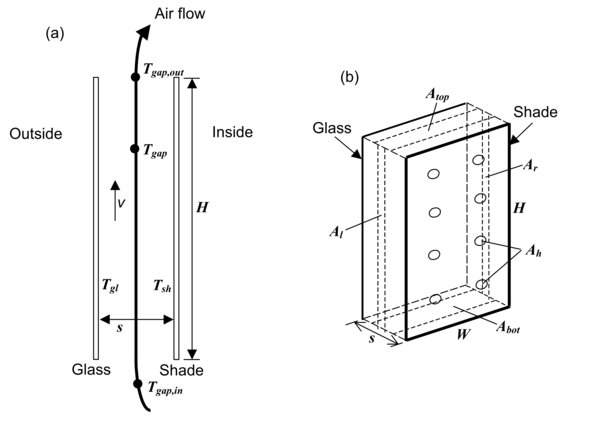
\includegraphics[width=0.9\textwidth, height=0.9\textheight, keepaspectratio=true]{media/image033.png}
\caption{Vertical section (a) and perspective view (b) of glass  and interior shade layers  showing variables used in the gap air flow analysis. In (b), the air-flow opening areas \(A_{\rm{bot}}\), \(A_{\rm{top}}\), \(A_{l}\), \(A_{r}\) and \(A_{h}\) are shown schematically. See \emph{Engineering Manual} for definition of thermal variables. \protect \label{fig:vertical-section-a-and-perspective-view-b-of}}
\end{figure}

\begin{figure}[hbtp] % fig 13
\centering
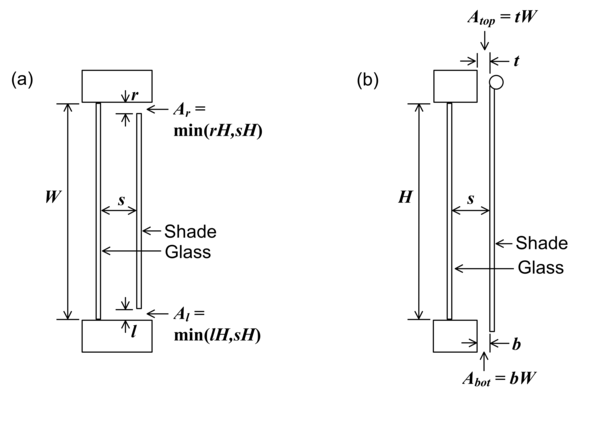
\includegraphics[width=0.9\textwidth, height=0.9\textheight, keepaspectratio=true]{media/image034.png}
\caption{Examples of air-flow openings for an interior shade covering glass of height \(H\) and width \(W\). Not to scale. (a) Horizontal section through shade with openings on the left and right sides (top view). (b) Vertical section through shade with openings at the top and bottom (side view). In (a) Left-Side Opening Multiplier = \(A_{l}/sH = min(l/s, 1)\) and Right-Side Opening Multiplier = \(A_{r}/sH = min(r/s, 1)\). In (b) Top Opening Multiplier = \(A_{\rm{top}}/sW = t/s\) and Bottom Opening Multiplier = \(A_{\rm{bot}}/sW = b/s\). \protect \label{fig:examples-of-air-flow-openings-for-an-interior}}
\end{figure}

An IDF example:

\begin{lstlisting}
WindowMaterial:Shade,
  DRAPES - CLOSE WEAVE MEDIUM,  !- Name
  0.05,                         !- Solar transmittance
  0.3000000,                    !- Solar Reflectance
  .05,                          !- Visible transmittance
  0.3000000,                    !- Visible reflectance
  0.9000000,                    !- Infrared Hemispherical Emissivity
  0.0,                          !- Infrared Transmittance
  0.003,                        !- Thickness {m}
  0.1,                          !- Conductivity {W/m-K}
  0.050,                        !- Shade to glass distance {m}
  1.0,                          !- Top opening multiplier
  1.0,                          !- Bottom opening multiplier
  0.0,                          !- Left-side opening multiplier
  0.0,                          !- Right-side opening multiplier
  0.0;                          !- Air flow permeability
\end{lstlisting}

\subsection{WindowMaterial:Blind}\label{windowmaterialblind}

This object specifies the properties of a window blind consisting of flat, equally-spaced slats. Unlike window shades, which are modeled as perfect diffusers, window blinds have solar and visible transmission and reflection properties that strongly depend on slat angle and angle of incidence of solar radiation. There is an EnergyPlus Reference Data Set for WindowMaterial:Blind that contains properties of generic window blinds.

Blinds can be located on the inside of the window (``interior blinds''), on the outside of the window (``exterior blinds''), or between two layers of glass (``between-glass blinds''). When in place, the blind is assumed to cover all of the glazed part of the window, including dividers; it does not cover any of the window frame, if present. The plane of the blind is assumed to be parallel to the glazing. When the blind is retracted it is assumed to cover none of the window. The solar and thermal effects of the blind's support strings, tapes or rods are ignored. Slat curvature, if present, is ignored.

There are two methods of assigning a blind to a window:

\subsubsection{Inputs}\label{inputs-23-005}

\paragraph{Method 1:}\label{method-1-1}
\begin{itemize}
\item 1) Define the construction of the window without the blind, the so-called ``bare'' construction.

\item 2) Reference the bare construction in the \hyperref[fenestrationsurfacedetailed]{FenestrationSurface:Detailed} for the window.

\item 3) Define the WindowMaterial:Blind.

\item 4) Define a \hyperref[windowpropertyshadingcontrol]{WindowShadingControl} for the window in which you (a) specify that this WindowMaterial:Blind is the window's shading device and (b) specify how the blind is controlled.

\end{itemize}

\paragraph{Method 2:}\label{method-2-1}

\begin{itemize}
\item 1) Define the Construction of the window without the blind, the so-called ``bare'' construction.

\item 2) Reference the bare construction in the \hyperref[fenestrationsurfacedetailed]{FenestrationSurface:Detailed} for the window.

\item 3) Define the WindowMaterial:Blind.

\item 4) Define another Construction, called the ``shaded construction,'' that includes the WindowMaterial:Blind.

\item[5)] Define a \hyperref[windowpropertyshadingcontrol]{WindowShadingControl} for the window in which you (a) reference the shaded construction and (b) specify how the blind is controlled.

Note that \hyperref[windowpropertyshadingcontrol]{WindowShadingControl} has to be used with either method, even if the blind is in place at all times. You will get an error message if you try to reference a construction with a blind directly from Window objects (\hyperref[fenestrationsurfacedetailed]{FenestrationSurface:Detailed} or Window).

Note also that \hyperref[windowpropertyshadingcontrol]{WindowShadingControl} is used to determine not only when the blind is in place, but how its slat angle is controlled.

\end{itemize}

\paragraph{Field: Name}\label{field-name-17-007}

Name of the blind. It is referenced as a layer in a window construction (ref: Construction object) or as a ``Material Name of Shading Device'' in a \hyperref[windowpropertyshadingcontrol]{WindowShadingControl} object.

\paragraph{Field: Slat Orientation}\label{field-slat-orientation}

The choices are Horizontal and Vertical. ``Horizontal'' means the slats are parallel to the bottom of the window; this is the same as saying that the slats are parallel to the X-axis of the window. ``Vertical'' means the slats are parallel to Y-axis of the window.

\paragraph{Field: Slat Width}\label{field-slat-width}

The width of the slat measured from edge to edge (m). See Figure~\ref{fig:a-side-view-of-a-window-blind-with-horizontal}.

\paragraph{Field: Slat Separation}\label{field-slat-separation}

The distance between the front of a slat and the back of the adjacent slat (m). See Figure~\ref{fig:a-side-view-of-a-window-blind-with-horizontal}.

\paragraph{Field: Slat Thickness}\label{field-slat-thickness}

The distance between the faces of a slat (m). See Figure~\ref{fig:a-side-view-of-a-window-blind-with-horizontal}.

\paragraph{Field: Slat Angle}\label{field-slat-angle}

The angle (degrees) between the glazing outward normal and the slat outward normal, where the outward normal points away from the front face of the slat (degrees). See Figure~\ref{fig:a-side-view-of-a-window-blind-with-horizontal}.

If the \hyperref[windowpropertyshadingcontrol]{WindowShadingControl} for the blind has Type of Slat Angle Control for Blinds = FixedSlatAngle, the slat angle is fixed at ``Slat Angle.''

If Type of Slat Angle Control for Blinds = BlockBeamSolar, the program automatically adjusts the slat angle so as just block beam solar radiation. In this case the value of ``Slat Angle'' is used only when the blind is in place and there is no beam solar radiation incident on the blind.

If Type of Slat Angle Control for Blinds = ScheduledSlatAngle, the slat angle is variable. In this case ``Slat Angle'' is not applicable and the field should be blank.

If Type of Slat Angle Control for Blinds = FixedSlatAngle and ``Slat Angle'' is less than the minimum or greater than the maximum allowed by Slat Width, Slat Separation and Slat Thickness, the slat angle will be reset to the corresponding minimum or maximum and a warning will be issued.

\paragraph{Field: Slat Conductivity}\label{field-slat-conductivity}

The thermal conductivity of the slat (W/m-K).

\paragraph{Field: Slat Beam Solar Transmittance}\label{field-slat-beam-solar-transmittance}

The beam solar transmittance of the slat, assumed to be independent of angle of incidence on the slat. Any transmitted beam radiation is assumed to be 100\% diffuse (i.e., slats are translucent).

\paragraph{Field: Front Side Slat Beam Solar Reflectance}\label{field-front-side-slat-beam-solar-reflectance}

The beam solar reflectance of the front side of the slat, assumed to be independent of angle of incidence (matte finish). This means that slats with a large specularly-reflective component (shiny slats) are not well modeled.

\paragraph{Field: Back Side Slat Beam Solar Reflectance}\label{field-back-side-slat-beam-solar-reflectance}

The beam solar reflectance of the back side of the slat, assumed to be independent of angle of incidence (matte finish). This means that slats with a large specularly-reflective component (shiny slats) are not well modeled.

\paragraph{Field: Slat Diffuse Solar Transmittance}\label{field-slat-diffuse-solar-transmittance}

The slat transmittance for hemispherically diffuse solar radiation. This value should equal ``Slat Beam Solar Transmittance.''

\paragraph{Field: Front Side Slat Diffuse Solar Reflectance}\label{field-front-side-slat-diffuse-solar-reflectance}

The front-side slat reflectance for hemispherically diffuse solar radiation. This value should equal ``Front Side Slat Beam Solar Reflectance.''

\paragraph{Field: Back Side Slat Diffuse Solar Reflectance}\label{field-back-side-slat-diffuse-solar-reflectance}

The back-side slat reflectance for hemispherically diffuse solar radiation. This value should equal ``Back Side Slat Beam Solar Reflectance.''

\paragraph{Field: Slat Beam Visible Transmittance}\label{field-slat-beam-visible-transmittance}

The beam visible transmittance of the slat, assumed to be independent of angle of incidence on the slat. Any transmitted visible radiation is assumed to be 100\% diffuse (i.e., slats are translucent).

\paragraph{Field: Front Side Slat Beam Visible Reflectance}\label{field-front-side-slat-beam-visible-reflectance}

The beam visible reflectance on the front side of the slat, assumed to be independent of angle of incidence (matte finish). This means that slats with a large specularly-reflective component (shiny slats) are not well modeled.

\paragraph{Field: Back Side Slat Beam Visible Reflectance}\label{field-back-side-slat-beam-visible-reflectance}

The beam visible reflectance on the front side of the slat, assumed to be independent of angle of incidence (matte finish). This means that slats with a large specularly-reflective component (shiny slats) are not well modeled.

\paragraph{Field: Slat Diffuse Visible Transmittance}\label{field-slat-diffuse-visible-transmittance}

The slat transmittance for hemispherically diffuse visible radiation. This value should equal ``Slat Beam Visible Transmittance.''

\paragraph{Field: Front Side Slat Diffuse Visible Reflectance}\label{field-front-side-slat-diffuse-visible-reflectance}

The front-side slat reflectance for hemispherically diffuse visible radiation. This value should equal ``Front Side Slat Beam Visible Reflectance.''

\paragraph{Field: Back Side Slat Diffuse Visible Reflectance}\label{field-back-side-slat-diffuse-visible-reflectance}

The back-side slat reflectance for hemispherically diffuse visible radiation. This value should equal ``Back Side Slat Beam Visible Reflectance..''

\paragraph{Field: Slat Infrared Hemispherical Transmittance}\label{field-slat-infrared-hemispherical-transmittance}

The slat Infrared transmittance. It is zero for solid metallic, wooden or glass slats, but may be non-zero in some cases (e.g., thin plastic slats).

\paragraph{Field: Front Side Slat Infrared Hemispherical Emissivity}\label{field-front-side-slat-infrared-hemispherical-emissivity}

Front-side hemispherical emissivity of the slat. Approximately 0.9 for most materials. The most common exception is bare (unpainted) metal slats or slats finished with a metallic paint.

\paragraph{Field: Back Side Slat Infrared Hemispherical Emissivity}\label{field-back-side-slat-infrared-hemispherical-emissivity}

Back-side hemispherical emissivity of the slat. Approximately 0.9 for most materials. The most common exception is bare (unpainted) metal slats or slats finished with a metallic paint.

\paragraph{Field: Blind to Glass Distance}\label{field-blind-to-glass-distance}

For interior and exterior blinds, the distance from the mid-plane of the blind to the adjacent glass (m). See Figure~\ref{fig:a-side-view-of-a-window-blind-with-horizontal}. Not used for between-glass blinds. As for window shades (ref: \hyperref[windowmaterialshade]{WindowMaterial:Shade}) this distance is used in calculating the natural convective air flow between glass and blind that is produced by buoyancy effects.

\paragraph{Opening Multipliers}\label{opening-multipliers}

The following opening multipliers are defined in the same way as for window shades (see \hyperref[windowmaterialshade]{WindowMaterial:Shade}, Figure~\ref{fig:vertical-section-a-and-perspective-view-b-of} and Figure~\ref{fig:examples-of-air-flow-openings-for-an-interior}). Note that, unlike window shades, there is no input for Air-Flow Permeability; this is automatically calculated by the program from slat angle, width and separation.

\paragraph{Field: Blind Top Opening Multiplier}\label{field-blind-top-opening-multiplier}

Defined as for Material:WindowShade.

\paragraph{Field: Blind Bottom Opening Multiplier}\label{field-blind-bottom-opening-multiplier}

Defined as for Material:WindowShade.

\paragraph{Field: Blind Left-Side Opening Multiplier}\label{field-blind-left-side-opening-multiplier}

Defined as for Material:WindowShade.

\paragraph{Field: Blind Right-Side Opening Multiplier}\label{field-blind-right-side-opening-multiplier}

Defined as for Material:WindowShade.

\paragraph{Field: Minimum Slat Angle}\label{field-minimum-slat-angle}

The minimum allowed slat angle (degrees). Used only if \hyperref[windowpropertyshadingcontrol]{WindowShadingControl} (for the window that incorporates this blind) varies the slat angle (i.e., the \hyperref[windowpropertyshadingcontrol]{WindowShadingControl} has Type of Slat Angle Control for Blinds = ScheduledSlatAngle or BlockBeamSolar). In this case, if the program tries to select a slat angle less than Minimum Slat Angle it will be reset to Minimum Slat Angle. (Note that if the Minimum Slat Angle itself is less than the minimum allowed by Slat Width, Slat Separation and Slat Thickness, it will be reset to that minimum.)

\paragraph{Field: Maximum Slat Angle}\label{field-maximum-slat-angle}

The maximum allowed slat angle (degrees). Used only if \hyperref[windowpropertyshadingcontrol]{WindowShadingControl} (for the window that incorporates this blind) varies the slat angle (i.e., the \hyperref[windowpropertyshadingcontrol]{WindowShadingControl} has Type of Slat Angle Control for Blinds = ScheduledSlatAngle or BlockBeamSolar). In this case, if the program tries to select a slat angle greater than Maximum Slat Angle the slat angle will be reset to Maximum Slat Angle. (Note that if the Maximum Slat Angle itself is greater than the maximum allowed by Slat Width, Slat Separation and Slat Thickness, it will be reset to that maximum.)

An IDF example:

\begin{lstlisting}

WindowMaterial:Blind,
   White Painted Metal Blind,   !- Name
   HORIZONTAL, !- Slat orientation
   0.025   , !- Slat width (m)
   0.01875 , !- Slat separation (m)
   0.001   , !- Slat thickness (m)
   45.0    , !- Slat angle (deg)
   44.9    , !- Slat conductivity (W/m-K)
   0.0     , !- Slat beam solar transmittance
   0.8     , !- Front Side Slat beam solar reflectance
   0.8     , !- Back Side Slat beam solar reflectance
   0.0     , !- Slat diffuse solar transmittance
   0.8     , !- Front Side Slat diffuse solar reflectance
   0.8     , !- Back Side Slat diffuse solar reflectance
   0.0     , !- Slat beam visible transmittance
   0.7     , !- Front Side Slat beam visible reflectance
   0.7     , !- Back Side Slat beam visible reflectance
   0.0     , !- Slat diffuse visible transmittance
   0.7     , !- Front Side Slat diffuse visible reflectance
   0.7     , !- Back Side Slat diffuse visible reflectance
   0.0     , !- Slat Infrared hemispherical transmittance
   0.9     , !- Front Side Slat Infrared hemispherical emissivity
   0.9     , !- Back Side Slat Infrared hemispherical emissivity
   0.050   , !- Blind-to-glass distance
   0.0     , !- Blind top opening multiplier
   0.0     , !- Blind bottom opening multiplier
   0.5     , !- Blind left-side opening multiplier
   0.5     , !- Blind right-side opening multiplier
   ,         !- Minimum slat angle (deg)
   ;         !- Maximum slat angle (deg)
\end{lstlisting}

\begin{figure}[hbtp] % fig 14
\centering
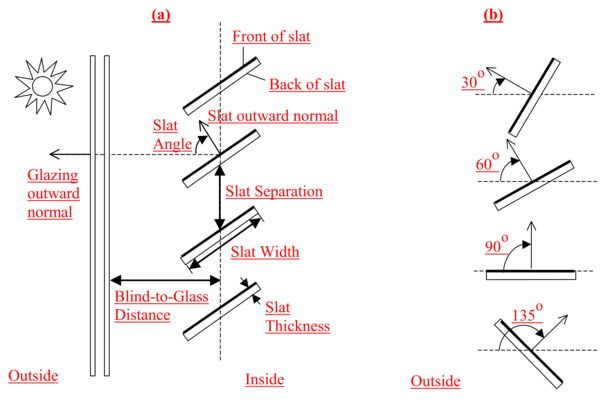
\includegraphics[width=0.9\textwidth, height=0.9\textheight, keepaspectratio=true]{media/image035.png}
\caption{(a) Side view of a window blind with horizontal slats (or top view of blind with vertical slats) showing slat geometry. The front face of a slat is shown by a heavy line. The slat angle is defined as the angle between the glazing outward normal and the slat outward normal, where the outward normal points away from the front face of the slat. (b) Slat orientations for representative slat angles. The slat angle varies from 0\(^{o}\), when the front of the slat is parallel to the glazing and faces toward the outdoors,  to 90\(^{o}\), when the slat is perpendicular to the glazing, to 180\(^{o}\), when the front of the slat is parallel to the glazing and faces toward the indoors. The minimum and maximum slat angles are determined by the slat thickness, width and separation. \protect \label{fig:a-side-view-of-a-window-blind-with-horizontal}}
\end{figure}

\subsection{WindowMaterial:ComplexShade}\label{windowmaterialcomplexshade}

This input object is used to define shade layers used in the \hyperref[constructioncomplexfenestrationstate]{Construction:ComplexFenestrationState} object.

\subsubsection{Inputs}\label{inputs-24-003}

\paragraph{Field: Name}\label{field-name-18-007}

Unique name of the shading layer.

\paragraph{Field: Shading Layer Type}\label{field-shading-layer-type}

The type of shading layer. The options are:

\begin{itemize}
\item
  VenetianHorizontal -- for modeling horizontal venetian blinds
\item
  VenetianVertical -- for modeling vertical venetian blinds
\item
  Woven -- for modeling shading systems with a regular weave
\item
  Perforated -- for modeling perforated screens
\item
  BSDF -- for modeling shades whose properties are represented by a BSDF file
\item
  OtherShadingType -- for modeling shading systems which do not belong to the any of the previous group
\end{itemize}

\paragraph{Field: Thickness}\label{field-thickness-7}

The thickness (m) of the shading layer. This value is ignored for ShadingLayerType = Venetian*, because the program will calculate the thickness based on the slat angle. This value is needed for ShadingLayerType = Woven and Perforated

\paragraph{Field: Conductivity}\label{field-conductivity-4}

The conductivity (W/mK) of the shading layer material. Default: 1.0

\begin{itemize}
\item
  Venetian* -- the conductivity of the venetian blind slat material
\item
  Woven -- the conductivity of the woven shade material (such as the thread for a fabric shade)
\item
  Perforated -- for modeling perforated screens
\item
  BSDF -- for modeling shades whose properties are represented by a BSDF file
\item
  OtherShadingType -- for modeling shading systems which do not belong to the any of the previous group
\end{itemize}

\paragraph{Field: IR Transmittance}\label{field-ir-transmittance}

The IR transmittance of the shading layer. Minimum value: 0. Maximum value: 1. Default: 0.

\paragraph{Field: Front Emissivity}\label{field-front-emissivity}

The front emissivity of the shading layer. Minimum value: > 0. Maximum value: 1. Default: 0.90.

\paragraph{Field: Back Emissivity}\label{field-back-emissivity}

The back emissivity of the shading layer. Minimum value: > 0. Maximum value: 1. Default: 0.90.

\paragraph{Field: Top Opening Multiplier}\label{field-top-opening-multiplier-1}

The top opening multiplier value will depend on the location of the shading device within the glazing system. There are several possible scenarios which can occur and they can be divided into two groups:

\textbf{Shading device on the indoor/outdoor side of the window}

In this case the opening multiplier is calculated as the smallest distance between the shading device and the frame (d\(_{top}\)), divided by the gap width (S). There are three possible cases for the position of a shading device the on indoor/outdoor side (see Figure~\ref{fig:three-cases-for-the-dp-calculation-for-an-indoor-outdoor-shade}).

\begin{figure}[htbp]
\centering
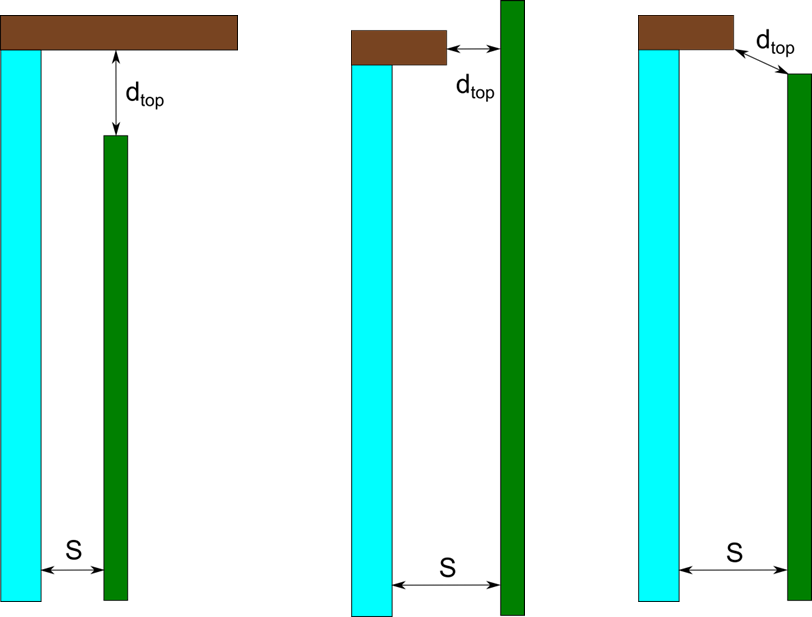
\includegraphics[width=0.9\textwidth, height=0.9\textheight, keepaspectratio=true]{media/three-cases-for-the-dtop-calculation-for-an-indoor-outdoor-shade-collage.png}
\caption{Three cases for the D\(_{top}\) calculation for an indoor/outdoor shade: Case a) A shading device between the frame; Case b) A shading device outside the frame, covering the frame; Case c) a shading device outside the frame, not covering the frame. \protect \label{fig:three-cases-for-the-dp-calculation-for-an-indoor-outdoor-shade}}
\end{figure}

In the case where the distance between the frame and the shading device is bigger than the gap width, the d\(_{top}\) multiplier is equal to one. Therefore, the calculation of the D\(_{top}\) opening multiplier is:

\begin{equation*}
A_{top} = min(d_{top}/S, 1)
\end{equation*}

\textbf{Shading device between glass layers}

In this case the opening multiplier is calculated as the smallest distance between the shading device and the frame or spacer (d\(_{top}\)), divided by the smaller gap width (the minimum of (S\(_{1}\) andS\(_{2}\))).

\begin{figure}[htbp]
\centering
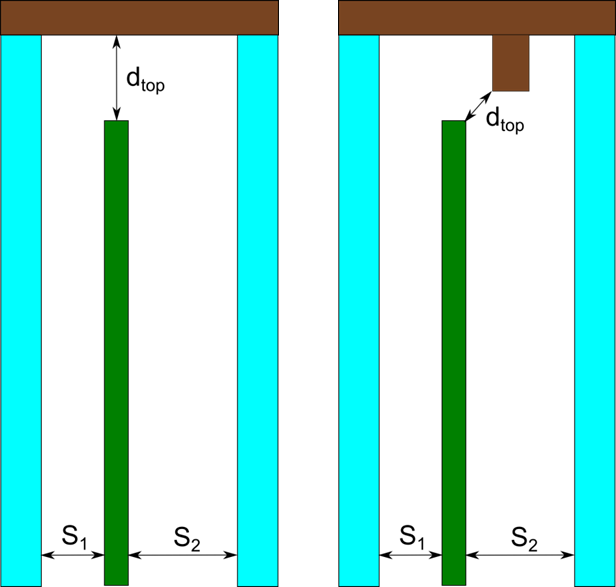
\includegraphics[width=0.9\textwidth, height=0.9\textheight, keepaspectratio=true]{media/calculation-of-dtop-for-a-shading-device-collage.png}
\caption{Calculation of Dtop for a shading device between glass layers \protect \label{fig:calculation-of-dtop-for-a-shading-device-between-glass-layers}}
\end{figure}

The D\(_{top}\) opening multiplier for a between glass shade is calculated as:

\begin{equation*}
A_{top} = min(d_{top}/S_{min}, 1)
\end{equation*}

Where

\begin{equation*}
S_{min} = min(S_1, S_2)
\end{equation*}

\paragraph{Field: Bottom Opening Multiplier}\label{field-bottom-opening-multiplier-1}

The bottom opening multiplier (d\(_{bot}\)) is calculated in the same way as the top opening multiplier, with the rules applied to the bottom of the shading device.

\paragraph{Field: Left Side Opening Multiplier}\label{field-left-side-opening-multiplier-1}

The left side opening multiplier (d\(_{left}\)) is calculated in the same way as the top opening multiplier, with the rules applied to the left side of the shading device.

\paragraph{Field: Right Side Opening Multiplier}\label{field-right-side-opening-multiplier-1}

The right side opening multiplier (d\(_{right}\)) is calculated in the same way as the top opening multiplier, with the rules applied to the right side of the shading device.

\paragraph{Field: Front Opening Multiplier}\label{field-front-opening-multiplier}

The fraction of glazing system area that is open on the front of the shading layer (see Figure~\ref{fig:front-view-of-shading-layer-openings.}). This fraction is calculated as follows: Afront / (W * H), where Afront = Area of the front of the glazing system that is not covered by the shading system, W = the width of the glazing system (IGU) and H is height of the glazing system (IGU).

\begin{figure}[hbtp] % fig 17
\centering
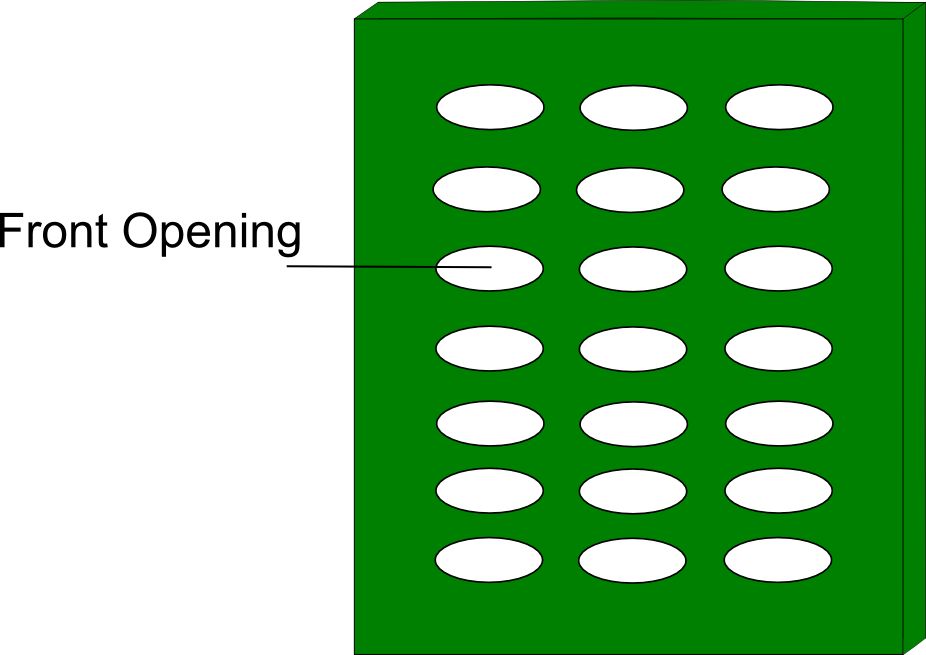
\includegraphics[width=0.9\textwidth, height=0.9\textheight, keepaspectratio=true]{media/image041.png}
\caption{Front view of shading layer openings. \protect \label{fig:front-view-of-shading-layer-openings.}}
\end{figure}

\paragraph{Field: Slat Width}\label{field-slat-width-1}

The width (m) of the venetian slats.~ Used only for ShadingLayerType = Venetian.

\paragraph{Field: Slat Spacing}\label{field-slat-spacing}

The distance (m) between front sides of the venetian slats.~ Used only for ShadingLayerType = Venetian.

\paragraph{Field: Slat Thickness}\label{field-slat-thickness-1}

The thickness (m) of the venetian slats.~ Used only for ShadingLayerType = Venetian.

\paragraph{Field: Slat Angle}\label{field-slat-angle-1}

The slat tilt angle (degrees) of the venetian slats.~ Used only for ShadingLayerType = Venetian.~ Range of slat angle is from -90 to 90 degrees.

\paragraph{Field: Slat Conductivity}\label{field-slat-conductivity-1}

The conductivity (W/mK) of the venetian slats.~ Used only for ShadingLayerType = Venetian.

\paragraph{Field: Slat Curve}\label{field-slat-curve}

The curvature radius (m) of the venetian slats.~ Setting this value to zero means there is no curvature in the slat (it is flat), while a non-zero value is the radius of the slat curve.~ This value cannot be smaller than Slat Width / 2.~ Used only for ShadingLayerType = Venetian.

\begin{figure}[hbtp] % fig 18
\centering
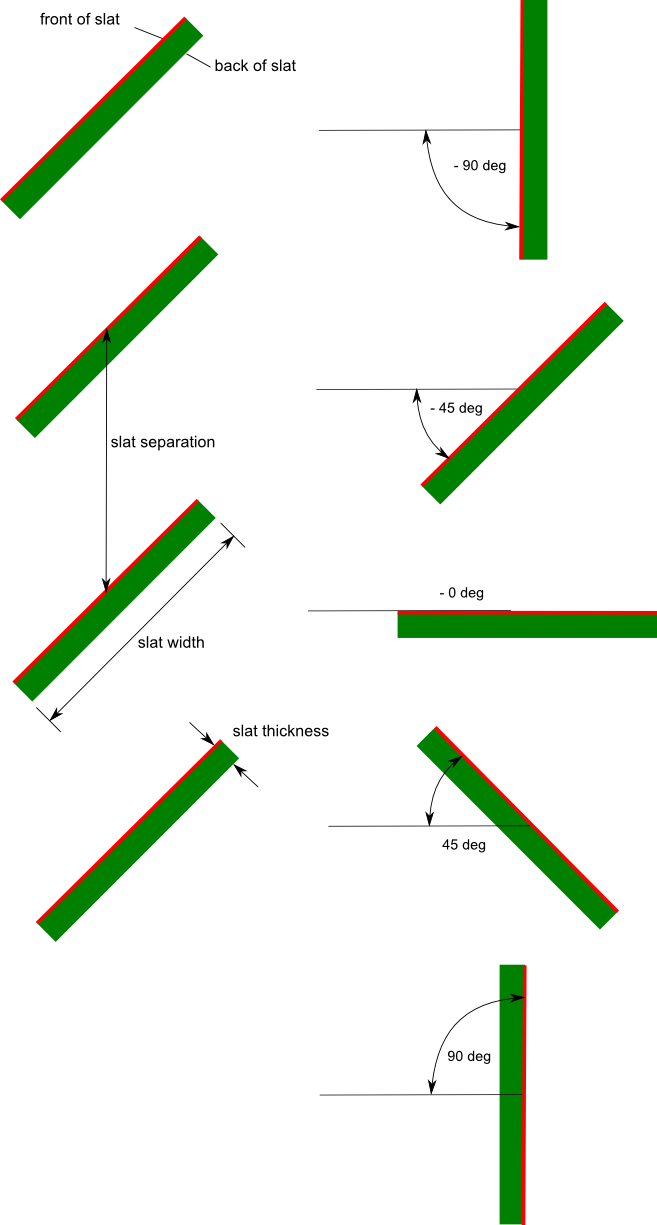
\includegraphics[width=0.9\textwidth, height=0.9\textheight, keepaspectratio=true]{media/image042.png}
\caption{Side view of horizontal venetian blind slats or top view of blinds with vertical slats.  Front face of slats is marked with red line. \protect \label{fig:side-view-of-horizontal-venetian-blind-slats}}
\end{figure}

An IDF example for ShadingLayerType = Venetian

\begin{lstlisting}

WindowMaterial:ComplexShade,       !- venetian blind layer
    Shade_30001_Layer,               !- name
    Venetian,                        !- shading layer type
    0.005,                           !- thickness
    160,                             !- layer conductivity
    0.0,                             !- IR transmittance
    0.9,                             !- front emissivity
    0.9,                             !- back emissivity
    0.0,                             !- top opening multiplier
    0.0,                             !- bottom opening multiplier
    0.0,                             !- left side opening multiplier
    0.0,                             !- right side opening multiplier
    0.05,                            !- front opening multiplier
    0.016,                           !- venetian slat width
    0.012,                           !- venetian slat spacing
    0.0006,                          !- venetian slat thickness
    -45.00,                          !- venetian slat angle
    160.00,                          !- venetian slat conductivity
    0.0000;                          !- venetian slat curve
\end{lstlisting}

An IDF example for ShadingLayerType = Woven

(Note that it is not necessary to include ``blank'' lines for the venetian blind input for a Woven shade definition).

\begin{lstlisting}

WindowMaterial:ComplexShade,       !- woven shade layer
    Shade_30002_Layer,               !- name
    Woven,                           !- shading layer type
    0.011,                           !- thickness
    1,                               !- layer conductivity
    0.0,                             !- IR transmittance
    0.9,                             !- front emissivity
    0.9,                             !- back emissivity
    0.0,                             !- top opening multiplier
    0.0,                             !- bottom opening multiplier
    0.0,                             !- left side opening multiplier
    0.0,                             !- right side opening multiplier
    0.17;                            !- front opening multiplier
\end{lstlisting}

\subsection{WindowMaterial:Screen}\label{windowmaterialscreen}

This object specifies the properties of exterior window screen materials. The window screen model assumes the screen is made up of intersecting orthogonally-crossed cylinders. The surface of the cylinders is assumed to be diffusely reflecting, having the optical properties of a Lambertian surface.

The beam solar radiation transmitted through a window screen varies with sun angle and is made up of two distinct elements: a direct beam component and a reflected beam component. The direct beam transmittance component is modeled using the geometry of the screen material and the incident angle of the sun to account for shadowing of the window by the screen material. The reflected beam component is an empirical model that accounts for the inward reflection of solar beam off the screen material surface. This component is both highly directional and small in magnitude compared to the direct beam transmittance component (except at higher incident angles, for which case the magnitude of the direct beam component is small or zero and the reflected beam component, though small in absolute terms can be many times larger than the direct beam component). For this reason, the reflected beam transmittance component calculated by the model can be a. disregarded, b. treated as an additive component to direct beam transmittance (and in the same direction), or c. treated as hemispherically-diffuse transmittance based on a user input to the model.

\begin{figure}[hbtp] % fig 19
\centering

\includegraphics[width=0.9\textwidth, height=0.9\textheight, keepaspectratio=true]{media/image043.png}
\caption{Direct beam and reflected beam transmittance components \protect \label{fig:direct-beam-and-reflected-beam-transmittance}}
\end{figure}

The window screen ``assembly'' properties of overall beam solar reflectance and absorptance (including the screen material `cylinders' and open area) also change with sun angle and are calculated based on the values of the beam solar transmittance components (direct and reflected components described above) and the physical properties of the screen material (i.e., screen material diameter, spacing, and reflectance).

Transmittance, reflectance, and absorptance of diffuse solar radiation are considered constant values and apply to both the front and back surfaces of the screen. These properties are calculated by the model as an average value by integrating the screen's beam solar properties over a quarter hemisphere of incident radiation. Long-wave emissivity is also assumed to be the same for both sides of the screen.

There is an EnergyPlus Reference Data Set for WindowMaterial:Screen that contains properties for generic window screens. Window screens of this type can only be used on the outside surface of the window (``exterior screens''). When in place, the screen is assumed to cover all of the glazed part of the window, including dividers; it does not cover any of the window frame, if present. The plane of the screen is assumed to be parallel to the glazing.

WindowMaterial:Screen can be used to model wire mesh insect screens where the solar and visible transmission and reflection properties vary with the angle of incidence of solar radiation. For diffusing materials such as drapery and translucent roller shades it is better to use the \hyperref[windowmaterialshade]{WindowMaterial:Shade} object. For slat-type shading devices like Venetian blinds, which have solar and visible transmission and reflection properties that strongly depend on slat angle and angle of incidence of solar radiation, it is better to use \hyperref[windowmaterialblind]{WindowMaterial:Blind}.

There are two methods of assigning a screen to a window:

\subsubsection{Inputs}\label{inputs-25-003}

\paragraph{Method 1:}\label{method-1-2}
\begin{itemize}
\item 1) Define the construction of the window without the screen, the so-called ``bare'' construction.

\item 2) Reference the bare construction in the \hyperref[fenestrationsurfacedetailed]{FenestrationSurface:Detailed} for the window.

\item 3) Define the WindowMaterial:Screen object.

\item 4) Define a \hyperref[windowpropertyshadingcontrol]{WindowShadingControl} for the window in which you (a) specify that this Material:WindowScreen is the window's shading device, and (b) specify how the screen is controlled.

\end{itemize}

\paragraph{Method 2:}\label{method-2-2}

\begin{itemize}
\item 1) Define the Construction of the window without the screen, the so-called ``bare'' construction.

\item 2) Reference the bare construction in the \hyperref[fenestrationsurfacedetailed]{FenestrationSurface:Detailed} for the window.

\item 3) Define the WindowMaterial:Screen object.

\item 4) Define another Construction, called the ``shaded construction,'' that includes the WindowMaterial:Screen.

\item 5) Define a \hyperref[windowpropertyshadingcontrol]{WindowShadingControl} for the window in which you (a) reference the shaded construction, and (b) specify how the screen is controlled.

Note that \hyperref[windowpropertyshadingcontrol]{WindowShadingControl} has to be used with either method, even if the screen is in place at all times. You will get an error message if you try to reference a shaded construction directly from a \hyperref[fenestrationsurfacedetailed]{FenestrationSurface:Detailed} object.

\end{itemize}

\paragraph{Field: Name}\label{field-name-19-004}

Enter a unique name for the screen. This name is referenced as an outside layer in a window construction.

\paragraph{Field: Reflected Beam Transmittance Accounting Method}\label{field-reflected-beam-transmittance-accounting-method}

This input specifies the method used to account for screen-reflected beam solar radiation that is transmitted through the window screen (as opposed to being reflected back outside the building). Since this inward reflecting beam solar is highly directional and is not modeled in the direction of the actual reflection, the user is given the option of how to account for the directionality of this component of beam solar transmittance. Valid choices are DoNotModel, ModelAsDirectBeam (i.e., model as an additive component to direct solar beam and in the same direction), or ModelAsDiffuse (i.e., model as hemispherically-diffuse radiation). The default value is ModelAsDiffuse.

\paragraph{Field: Diffuse Solar Reflectance}\label{field-diffuse-solar-reflectance}

This input specifies the solar reflectance (beam-to-diffuse) of the screen material itself (not the effective value for the overall screen ``assembly'' including open spaces between the screen material). The outgoing diffuse radiation is assumed to be Lambertian (distributed angularly according to Lambert's cosine law). The solar reflectance is assumed to be the same for both sides of the screen. This value must be from 0 to less than 1.0. In the absence of better information, the input value for diffuse solar reflectance should match the input value for diffuse visible reflectance.

\paragraph{Field: Diffuse Visible Reflectance}\label{field-diffuse-visible-reflectance}

This input specifies the visible reflectance (beam-to-diffuse) of the screen material itself (not the effective value for the overall screen ``assembly'' including open spaces between the screen material) averaged over the solar spectrum and weighted by the response of the human eye. The outgoing diffuse radiation is assumed to be Lambertian (distributed angularly according to Lambert's cosine law). The visible reflectance is assumed to be the same for both sides of the screen. This value must be from 0 to less than 1.0.

If diffuse visible reflectance for the screen material is not available, then the following guidelines can be used to estimate this value:

\begin{itemize}
\item
  Dark-colored screen (e.g., charcoal):~~~~~~~~~~~~~~~~~ 0.08 -- 0.10
\item
  Medium-colored screen (e.g., gray):~~~~~~~~~~~~~~~~~~ 0.20 -- 0.25
\item
  Light-colored screen (e.g., bright aluminum):~~~~~~ 0.60 -- 0.65
\end{itemize}

Commercially-available gray scale or grayscale reflecting chart references can be purchased for improved accuracy in estimating visible reflectance (by visual comparison of screen reflected brightness with that of various known-reflectance portions of the grayscale).

\paragraph{Field: Thermal Hemispherical Emissivity}\label{field-thermal-hemispherical-emissivity-1}

Long-wave emissivity \(\varepsilon\) of the screen material itself (not the effective value for the overall screen ``assembly'' including open spaces between the screen material). The emissivity is assumed to be the same for both sides of the screen.

For most non-metallic materials, \(\varepsilon\) is about 0.9. For metallic materials, \(\varepsilon\) is dependent on material, its surface condition, and temperature. Typical values for metallic materials range from 0.05--0.1 with lower values representing a more finished surface (e.g.~low oxidation, polished surface). Material emissivities may be found in Table 5 from the 2005 ASHRAE Handbook of Fundamentals, page 3.9. The value for this input field must be between 0 and 1, with a default value of 0.9 if this field is left blank.

\paragraph{Field: Conductivity}\label{field-conductivity-5}

Screen material conductivity (W/m-K). This input value must be greater than 0. The default value is 221 W/m-K (aluminum).

\paragraph{Field: Screen Material Spacing}\label{field-screen-material-spacing}

The spacing, S, of the screen material (m) is the distance from the center of one strand of screen to the center of the adjacent one. The spacing of the screen material is assumed to be the same in both directions (e.g., vertical and horizontal). This input value must be greater than the non-zero screen material diameter. If the spacing is different in the two directions, use the average of the two values.

\begin{figure}[hbtp] % fig 20
\centering
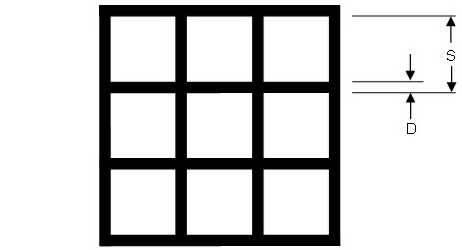
\includegraphics[width=0.9\textwidth, height=0.9\textheight, keepaspectratio=true]{media/image044.png}
\caption{Screen Material Spacing and Diameter \protect \label{fig:screen-material-spacing-and-diameter}}
\end{figure}

\paragraph{Field: Screen Material Diameter}\label{field-screen-material-diameter}

The diameter, D, of individual strands or wires of the screen material (m). The screen material diameter is assumed to be the same in both directions (e.g., vertical and horizontal). This input value must be greater than 0 and less than the screen material spacing. If the diameter is different in the two directions, use the average of the two values.

\paragraph{Field: Screen to Glass Distance}\label{field-screen-to-glass-distance}

Distance from the window screen to the adjacent glass surface (m). If the screen is not flat, the average screen to glass distance should be used. The screen-to-glass distance is used in calculating the natural convective air flow between the glass and the screen produced by buoyancy effects. This input value must be from 0.001 m to 1 m, with a default value of 0.025 m if this field is left blank.

\paragraph{Field: Top Opening Multiplier}\label{field-top-opening-multiplier-2}

Effective area for air flow at the top of the screen divided by the horizontal area between the glass and screen (see the same field for the Material:WindowShade object for additional description). The opening multiplier fields can be used to simulate a shading material that is offset from the window frame. Since window screens are typically installed against the window frame, the default value is equal to 0.This input value can range from 0 to 1.

\paragraph{Field: Bottom Opening Multiplier}\label{field-bottom-opening-multiplier-2}

Effective area for air flow at the bottom of the screen divided the horizontal area between the glass and screen (see the same field for the Material:WindowShade object for additional description). The opening multiplier fields can be used to simulate a shading material that is offset from the window frame. Since window screens are typically installed against the window frame, the default value is equal to 0. This input value can range from 0 to 1.

\paragraph{Field: Left-Side Opening Multiplier}\label{field-left-side-opening-multiplier-2}

Effective area for air flow at the left side of the screen divided the vertical area between the glass and screen (see the same field for the Material:WindowShade object for additional description). The opening multiplier fields can be used to simulate a shading material that is offset from the window frame. Since window screens are typically installed against the window frame, the default value is equal to 0. This input value can range from 0 to 1.

\paragraph{Field: Right-Side Opening Multiplier}\label{field-right-side-opening-multiplier-2}

Effective area for air flow at the right side of the screen divided the vertical area between the glass and screen (see the same field for the Material:WindowShade object for additional description). The opening multiplier fields can be used to simulate a shading material that is offset from the window frame. Since window screens are typically installed against the window frame, the default value is equal to 0. This input value can range from 0 to 1.

\paragraph{Field: Angle of Resolution for Screen Transmittance Output Map}\label{field-angle-of-resolution-for-screen-transmittance-output-map}

Angle of resolution, in degrees, for the overall screen beam transmittance (direct and reflected) output map. The comma-separated variable file eplusscreen.csv (Ref. OutputDetailsandExamples.pdf) will contain the direct beam and reflected beam solar radiation that is transmitted through the window screen as a function of incident sun angle (0 to 90 degrees relative solar azimuth and 0 to 90 degrees relative solar altitude) in sun angle increments specified by this input field. The default value is 0, which means no transmittance map is generated. Other valid choice inputs are 1, 2, 3 and 5 degrees.

An IDF example for this object, along with Construction and \hyperref[windowpropertyshadingcontrol]{WindowShadingControl} objects, is shown below:

\begin{lstlisting}

WindowMaterial:Screen,
      EXTERIOR SCREEN,         !- Name
      ModelAsDiffuse,        !- Reflected Beam Transmittance Accounting Method
      0.6,                     !- Diffuse Solar Reflectance
      0.6,                     !- Diffuse Visible Reflectance
      0.9,                     !- Thermal Hemispherical Emissivity
      221.0,                   !- Conductivity {W/m-K}
      0.00154,                 !- Screen Material Spacing (m)
      0.000254,                !- Screen Material Diameter (m)
      0.025,                   !- Screen-to-Glass Distance {m}
      0.0,                     !- Top Opening Multiplier
      0.0,                     !- Bottom Opening Multiplier
      0.0,                     !- Left-Side Opening Multiplier
      0.0,                     !- Right-Side Opening Multiplier
      0;                   !- Angle of Resolution for Output Map {deg}

  Construction,
      DOUBLE PANE WITHOUT SCREEN,     !- Name
      GLASS - CLEAR SHEET 1 / 8 IN,   !- Outside Layer
      WinAirB1 - AIRSPACE RESISTANCE, !- Layer \#2
      GLASS - CLEAR SHEET 1 / 8 IN;   !- Layer \#3

  WindowShadingControl,
      DOUBLE PANE WITH SCREEN, !- Name
      West Zone,               !- Zone Name
      1,                       !- Shading Control Sequence Number
      ExteriorScreen,          !- Shading Type
      ,                        !- Name of construction with shading
      AlwaysOn,                !- Shading Control Type
      ScreenSchedule,          !- Schedule Name
      20.0,                    !- SetPoint {W/m2, W or deg C}
      YES,                     !- Shading Control Is Scheduled
      NO,                      !- Glare Control Is Active
      EXTERIOR SCREEN,         !- Material Name of Shading Device
      ,                        !- Type of Slat Angle Control for Blinds
      ,                        !- Slat Angle Schedule Name
      ,                        !- Setpoint 2 {W/m2, deg C or cd/m2}
      ,                        !- Daylighting Control Object Name
      Sequential,              !- Multiple Surface Control Type
      Zn001:Wall001:Win001;    !- Fenestration Surface 1 Name
\end{lstlisting}

\subsection{WindowMaterial:Shade:EquivalentLayer}\label{windowmaterialshadeequivalentlayer}

This object specifies the properties of Equivalent Layer window shade (roller blind) materials. Shades are considered to be thin, flat and perfect diffusers (all transmitted and reflected radiation is hemispherically-diffuse). However, shades can have beam-beam transmittance by virtue of their material openness.~ The beam-beam transmittence is assumed to be the same for both sides of the shade and is the same as the openness area fraction. Beam-diffuse transmittance and reflectance, and emissivity properties can be different for front and back side of the shade.Window shades can be placed on the inside of the window, on the outside of the window, or between glass layers. WindowMaterial:Shade:EquivalentLayer is used for roller blinds. The off-normal solar property calculation of shades (roller blind) is based on a set of correlations developed from measurement of samples of commercially produced roller blind material with openness fraction less than 0.14. The model is not intended for materials with unusually high values of openness and should be limited to a maximum openness fraction of 0.20. The visible spectrum solar properties input fields are not used currently hence can be left blank. The equivalent layer window shade model does not support \hyperref[windowpropertyshadingcontrol]{WindowShadingControl}.

\subsubsection{Inputs}\label{inputs-26-002}

\paragraph{Field: Name}\label{field-name-20-003}

Name of the shade. It is referenced as an inside, inbetween or outside layer in an equivalent layer~ window construction.

\paragraph{Field: Shade Beam-Beam Solar Transmittance}\label{field-shade-beam-beam-solar-transmittance}

This value is the beam-beam transmittance of the shade at normal incidence and it is the same as the openness area fraction of the shade material. Assumed to be the same for front and back sides of the roller blinds.~ The minimum value is 0.0 and maximum value is less than 1.0.~ The default value is 0.0. For most common shade materials (e.g.~Roller Blinds) the material oppeness fraction doesn't exceed 0.20.

\paragraph{Field: Front Side Shade Beam-Diffuse Solar Transmittance}\label{field-front-side-shade-beam-diffuse-solar-transmittance}

This value is the front side beam-diffuse transmittance of the shade material at normal incidence averaged over the entire spectrum of solar radiation. The minimum value is 0.0 and maximum value is less than 1.0.~ The default value is 0.0.

\paragraph{Field: Back Side Shade Beam-Diffuse Solar Transmittance}\label{field-back-side-shade-beam-diffuse-solar-transmittance}

This value is the back side beam-diffuse transmittance of the shade material at normal incidence averaged over the entire spectrum of solar radiation. The minimum value is 0.0 and maximum value is less than 1.0.~ The default value is 0.0.

\paragraph{Field: Front Side Shade Beam-Diffuse Solar Reflectance}\label{field-front-side-shade-beam-diffuse-solar-reflectance}

This value is the front side beam-diffuse reflectance of the shade material at normal incidence averaged over the entire spectrum of solar radiation. The minimum value is 0.0 and maximum value is less than 1.0.

\paragraph{Field: Back Side Shade Beam-Diffuse Solar Reflectance}\label{field-back-side-shade-beam-diffuse-solar-reflectance}

This value is the back side beam-diffuse reflectance of the shade material at normal incidence averaged over the entire spectrum of solar radiation. The minimum value is 0.0 and maximum value is less than 1.0.

\paragraph{Field: Shade Beam-Beam Visible Transmittance}\label{field-shade-beam-beam-visible-transmittance}

This value is the beam-beam transmittance at normal incidence averaged over the visible spectrum of solar radiation. Assumed to be the same for front and back sides. The minimum value is 0.0 and maximum value is less than 1.0.~ Currently this input field is not used.

\paragraph{Field: Shade Beam-Diffuse Visible Transmittance}\label{field-shade-beam-diffuse-visible-transmittance}

This value is the beam-diffuse transmittance at normal incidence averaged over the visible spectrum of solar radiation. Assumed to be the same for front and back sides. The minimum value is 0.0 and maximum value is less than 1.0.~ Currently this input field is not used.

\paragraph{Field: Shade Beam-Diffuse Visible Reflectance}\label{field-shade-beam-diffuse-visible-reflectance}

This value is the beam-diffuse reflectance at normal incidence averaged over the visible spectrum of solar radiation. Assumed to be the same for front and back sides. The minimum value is 0.0 and maximum value is less than 1.0.~ Currently this input field is not used.

\paragraph{Field: Shade Material Infrared Transmittance}\label{field-shade-material-infrared-transmittance}

This value is the long-wave transmittance of the shade material and assumed to be the same for front and back sides of the shade. The minimum value is 0.0 and maximum value is less than 1.0. Default value is 0.05.

\paragraph{Field: Front Side Shade Material Infrared Emissivity}\label{field-front-side-shade-material-infrared-emissivity}

This value is the front side long-wave hemispherical emissivity of shade material. The minimum value is 0.0 and maximum value is less than 1.0. Default value is 0.91. The front side effective emissivity of the shade layer is calculated using this value and the material openness specified above.

\paragraph{Field: Back Side Shade Material Infrared Emissivity}\label{field-back-side-shade-material-infrared-emissivity}

This value is the back side long-wave hemispherical emissivity of shade material. The minimum value is 0.0 and maximum value is less than 1.0. Default value is 0.91. The back side effective emissivity of the shade is calculated using this value and the material openness specified above.

An IDF example for this object is shown below:

\begin{lstlisting}

WindowMaterial:Shade:EquivalentLayer,
    Shade1,        !- Name
    0.190,         !- Shade Beam-Beam Solar Transmittance
    0.206,         !- Front Side Shade Beam-Diffuse Solar Transmittance
    0.206,         !- Back Side Shade Beam-Diffuse Solar Transmittance
    0.499,         !- Front Side Shade Beam-Diffuse Solar Reflectance
    0.499,         !- Back Side Shade Beam-Diffuse Solar Reflectance
    0.0,           !- Shade Beam-Beam Visible Transmittance
    0.0,           !- Shade Beam-Diffuse Visible Transmittance
    0.0,           !- Shade Visible Reflectance
    0.0,           !- Shade Material Infrared Transmittance
    0.84,          !- Front Side Shade Material Infrared Emissivity
    0.84;          !- Back Side Shade Material Infrared Emissivity
\end{lstlisting}

\subsection{WindowMaterial:Drape:EquivalentLayer}\label{windowmaterialdrapeequivalentlayer}

Specifies the optical and thermal properties of equivalent layer window drape fabric materials.

Drapery fabric shades are commonly placed on the the inside of the window. The long-wave (Thermal) properties for commonly used drapery fabrics are assumed to be the same on both sides but different values can be specified when required. Drape fabric shade layers are considered to be perfect diffusers (reflected radiation is hemispherically-diffuse independent of angle of incidence). Unpleated drape fabric is treated as thin and flat layer.The off-normal optical properties of drapery fabric is determined from user specified optical properties at normal incidence using empirical correlations. Pleated drape fabric requires entering the pleated section average width and length as shown in Figure~\ref{fig:geometry-used-for-pleated-drape-analysis}. For pleated drapes the effective beam-beam and beam-diffuse solar properties are determined by tracking both radiation components, for a given incident angle solar radiation, through various interactions with a fabric pleated in a rectangular geometry shown in Figure~\ref{fig:geometry-used-for-pleated-drape-analysis}.~ The solar properties of the two different pleat facets are evaluated on the basis of the local solar incidence angle.~ Therefore, the effective layer properties are influenced not just by horizontal solar profile angle, but also by incidence angle. The correlations used for drape fabrics optical property calculations reqiure that the solar absorptance of the fabric, at normal incidence, is not less than 1\%. The equivalent layer window drapery fabric shade model does not support \hyperref[windowpropertyshadingcontrol]{WindowShadingControl}.

\begin{figure}[hbtp] % fig 21
\centering
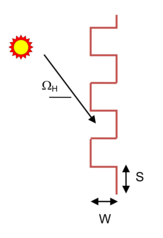
\includegraphics[width=0.9\textwidth, height=0.9\textheight, keepaspectratio=true]{media/image045.png}
\caption{Geometry used for Pleated Drape Analysis \protect \label{fig:geometry-used-for-pleated-drape-analysis}}
\end{figure}

\subsubsection{Inputs}\label{inputs-27-002}

\paragraph{Field: Name}\label{field-name-21-003}

Name of the drape fabric shade layer. It is referenced as an inside, in between or outside layer in an equivalent layer window construction.

\paragraph{Field: Drape Beam-Beam Solar Transmittance}\label{field-drape-beam-beam-solar-transmittance}

This value is the drape fabric beam-beam transmittance at normal incidence, and it is the same as the drape fabric openness area fraction.~ Assumed to be the same for front and back sides of the drape fabric layer.~ The minimum value is 0.0 and maximum value is less than 1.0. For most drape fabric materials the maximum fabric openness fraction do not exceed 0.2.~ The default value is 0.0.

\paragraph{Field: Front Side Drape Beam-Diffuse Solar Transmittance}\label{field-front-side-drape-beam-diffuse-solar-transmittance}

This value is the front side beam-diffuse solar transmittance of the drape fabric material at normal incidence averaged over the entire spectrum of solar radiation. The minimum value is 0.0 and maximum value is less than 1.0.

\paragraph{Field: Back Side Drape Beam-Diffuse Solar Transmittance}\label{field-back-side-drape-beam-diffuse-solar-transmittance}

This value is the back side beam-diffuse solar transmittance of the drape fabric material at normal incidence averaged over the entire spectrum of solar radiation. The minimum value is 0.0 and maximum value is less than 1.0.

\paragraph{Field: Front Side Drape Beam-Diffuse Solar Reflectance}\label{field-front-side-drape-beam-diffuse-solar-reflectance}

This value is the front side beam-diffuse solar reflectance of the drape fabric material at normal incidence averaged over the entire spectrum of solar radiation. The minimum value is 0.0 and maximum value is less than 1.0.

\paragraph{Field: Back Side Drape Beam-Diffuse Solar Reflectance}\label{field-back-side-drape-beam-diffuse-solar-reflectance}

This value is the back side beam-diffuse solar reflectance of the drape fabric material at normal incidence averaged over the entire spectrum of solar radiation. The minimum value is 0.0 and maximum value is less than 1.0.

\paragraph{Field: Drape Beam-Beam Visible Transmittance}\label{field-drape-beam-beam-visible-transmittance}

This value is the drape fabric beam-beam visible transmittance at normal incidence averaged over the visible spectrum range of solar radiation.~ Assumed to be the same for front and back sides of the drape fabric layer.~ The minimum value is 0.0 and maximum value is less than 1.0.~ The default value is 0.0.~ This input field is not used currently.

\paragraph{Field: Front Side Drape Beam-Diffuse Visible Reflectance}\label{field-front-side-drape-beam-diffuse-visible-reflectance}

This value is the front side drape fabric beam-diffuse visible reflectance at normal incidence averaged over the visible spectrum range of solar radiation.~ Assumed to be the same for front and back sides of the drape.~ The minimum value is 0.0 and maximum value is less than 1.0.~ The default value is 0.0.~ This input field is not used currently.

\paragraph{Field: Back Side Drape Diffuse-Diffuse Visible Reflectance}\label{field-back-side-drape-diffuse-diffuse-visible-reflectance}

This value is the back side drape fabric diffuse-diffuse visible reflectance at normal incidence averaged over the visible spectrum range of solar radiation.~ Assumed to be the same for front and back sides of the drape.~ The minimum value is 0.0 and maximum value is less than 1.0.~ The default value is 0.0.~ This input field is not used currently.

\paragraph{Field: Drape Material Infrared Transmittance}\label{field-drape-material-infrared-transmittance}

This value is the long-wave hemispherical transmittance of the fabric material at zero fabric openness fraction.~ Assumed to be the same for front and back sides of the drape fabric material layer. The minimum value is 0.0 and maximum value is less than 1.0.~ The default value is 0.05.

\paragraph{Field: Front Side Drape Material Infrared Emissivity}\label{field-front-side-drape-material-infrared-emissivity}

This value is the front side long-wave hemispherical emissivity of fabric material at zero shade openness. The minimum value is 0.0 and maximum value is less than 1.0. the default value is 0.87. The front side effective emissivity of the drape fabric layer is calculated using this value and the fabric openness area fraction specified above.

\paragraph{Field: Back Side Drape Material Infrared Emissivity}\label{field-back-side-drape-material-infrared-emissivity}

This value is the back side long-wave hemispherical emissivity of fabric material at zero fabric openness fraction. The minimum value is 0.0 and maximum value is less than 1.0. The default value is 0.87. The back side effective emissivity of the drape fabric layer is calculated using this value and the fabric openness area fraction specified above.

\paragraph{Field: Width of Pleated Fabric}\label{field-width-of-pleated-fabric}

This value is the width of the pleated section of the draped fabric, w(m). If the drape fabric is flat (unpleated), then the pleated section width is set to zero. The default value is 0.0, i.e., assumes flat drape fabric.

\paragraph{Field: Length of Pleated Fabric}\label{field-length-of-pleated-fabric}

This value is the length of the pleated section of the draped fabric, s(m). If the drape fabric is flat (unpleated), then the pleated section length is set to zero.~ The default value is 0.0, i.e., assumes flat drape fabric.

An IDF example for this object is shown below:

\begin{lstlisting}
WindowMaterial:Drape:EquivalentLayer,
  Drape02,            !- Name
  0.14,               !- Shade Beam-Beam Solar Transmittance
  0.10,               !- Front Side Shade Beam-Diffuse Solar Transmittance
  0.10,               !- Back Side Shade Beam-Diffuse Solar Transmittance
  0.40,               !- Front Side Shade Beam-Diffuse Solar Reflectance
  0.50,               !- Back Side Shade Beam-Diffuse Solar Reflectance
  0.0,                !- Shade Beam-Beam Visible Transmittance
  0.0,                !- Shade Beam-Diffuse Visible Transmittance
  0.0,                !- Shade Beam-Diffuse Visible Reflectance
  0.10,               !- Shade Material Infrared Transmittance
  0.90,               !- Front Side Shade Material Infrared Emissivity
  0.80,               !- Back Side Shade Material Infrared Emissivity
  0.01,               !- Width of Pleated Fabric
  0.025;              !- Length of Pleated Fabric
\end{lstlisting}

\subsection{WindowMaterial:Blind:EquivalentLayer}\label{windowmaterialblindequivalentlayer}

This object specifies the properties of an Equivalent Layer window blind consisting of thin and equally-spaced slats. The model assumes that slats are flat and thin, and applies correction for the slat curvature effect based on the user specified slat crown. Slats are assumed to transmit and reflect diffusely. The effective shortwave optical and longwave optical properties of venetian blind layer is estimated analytically. The Equivalent Layer blind model requires optical properties and geometry of the slats shown in Figure~\ref{fig:geometry-and-properties-used-for-venetian}. Likewise, effective longwave properties are obtained for the layer knowing longwave properties of the slats.

\begin{figure}[hbtp] % fig 22
\centering
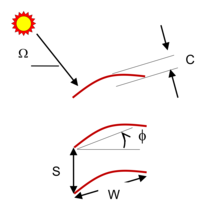
\includegraphics[width=0.9\textwidth, height=0.9\textheight, keepaspectratio=true]{media/image047.png}
\caption{Geometry and Properties used for venetian blind analysis \protect \label{fig:geometry-and-properties-used-for-venetian}}
\end{figure}

The input data required to characterize a venetian blind are: front and back side reflectance and transmittance of the slat, geometry (Slat width, w, slat spacing, s, slat crown, c, and slat angle, $\phi$, and long wave emittance and transmittance of the slat. Blinds can be located on the inside of the window, on the outside of the window, or between two layers of glass. The blind is assumed to cover all of the glazed part of the window.
The equivalent layer window blind model allows three slat angle control types (see \textit{Slat Angle Control} input field) but does not support \hyperref[windowpropertyshadingcontrol]{WindowShadingControl}.

\subsubsection{Inputs}\label{inputs-28-001}

\paragraph{Field: Name}\label{field-name-22-003}

Name of the venetian blind. It is referenced as an inside, outside or in between layers in an equivalent layer window construction.

\paragraph{Field: Slat Orientation}\label{field-slat-orientation-1}

The choices are Horizontal and Vertical. ``Horizontal'' means the slats are parallel to the bottom of the window; this is the same as saying that the slats are parallel to the X-axis of the window. ``Vertical'' means the slats are parallel to Y-axis of the window. The default is ``Horizontal''.

\paragraph{Field: Slat Width}\label{field-slat-width-2}

This value is the width of the slat measured from edge to edge (m). The default value is 0.0254.

\paragraph{Field: Slat Separation}\label{field-slat-separation-1}

The distance between the front of a slat and the back of the adjacent slat (m). The default value is 0.025. The slat separation should not be greater than the slat width.

\paragraph{Field: Slat Crown}\label{field-slat-crown}

The perpendicular length between the slat cord ~and the curve (m). Crown = 0.0625x``Slat width''. Slat is assumed to be rectangular in cross section and flat. The crown accounts for curvature of the slat.~ The minimum value is 0.0, and the default value is 0.0015m.

\paragraph{Field: Slat Angle}\label{field-slat-angle-2}

The angle (degrees) between the glazing outward normal and the slat outward normal, where the outward normal points away from the front face of the slat (degrees). The slat angle is +ve if the tip of the slat front face is tilted upward, or else the slat angle is -ve if the tip of the slat front face is tilted downward. The slat angle varies between -90 to +90.~ If the \textit{`Slat Angle Control} input field below specified is ``FixedSlatAngle'', then the slat angle is fixed at ``Slat Angle'' value entered.~ Minimum value allowed is -90.0, and the maximum value allowed is 90.0 degrees.~ The default value is 45 degrees.

\paragraph{Field: Front Side Slat Beam-Diffuse Solar Transmittance}\label{field-front-side-slat-beam-diffuse-solar-transmittance}

This value is the slat front side beam-diffuse solar transmittance at normal incidence averaged over the entire spectrum of solar radiation. Any transmitted beam radiation is assumed to be 100\% diffuse (i.e., slats are translucent). Minimum value is 0.0, and the maximum value is less than 1.0. The default value is 0.0.

\paragraph{Field: Back Side Slat Beam-Diffuse Solar Transmittance}\label{field-back-side-slat-beam-diffuse-solar-transmittance}

This value is the slat back side beam-diffuse solar transmittance at normal incidence averaged over the entire spectrum of solar radiation. Any transmitted beam radiation is assumed to be 100\% diffuse (i.e., slats are translucent). Minimum value is 0.0,~ and the maximum value is less than 1.0. The default value is 0.0.

\paragraph{Field: Front Side Slat Beam-Diffuse Solar Reflectance}\label{field-front-side-slat-beam-diffuse-solar-reflectance}

This value is slat front side beam-diffuse solar reflectance at normal incidence averaged over the entire spectrum of solar radiation. All the reflected component is assumed to be diffuse. Minimum value is 0.0, and the maximum value is less than 1.0.

\paragraph{Field: Back Side Slat Beam-Diffuse Solar Reflectance}\label{field-back-side-slat-beam-diffuse-solar-reflectance}

This value is the slat back side beam-diffuse solar reflectance at normal incidence averaged over the entire spectrum of solar radiation. All the reflected component is assumed to be diffuse. Minimum value is 0.0, and the maximum value is less than 1.0.

\paragraph{Field: Front Side Slat Beam-Diffuse Visible Solar Transmittance}\label{field-front-side-slat-beam-diffuse-visible-solar-transmittance}

This value is the slat front side beam-diffuse visible transmittance at normal incidence averaged over the visible spectrum range of solar radiation. Any transmitted beam radiation is assumed to be 100\% diffuse (i.e., slats are translucent). Minimum value is 0.0, and the maximum value is less than 1.0. The default value is 0.0.

\paragraph{Field: Back Side Slat Beam-Diffuse Visible Solar Transmittance}\label{field-back-side-slat-beam-diffuse-visible-solar-transmittance}

This value is the slat back side beam-diffuse visible transmittance at normal incidence averaged the visible spectrum range of solar radiation. Any transmitted beam radiation is assumed to be 100\% diffuse (i.e., slats are translucent). Minimum value is 0.0, and the maximum value is less than 1.0. The default value is 0.0.

\paragraph{Field: Front Side Slat Beam-Diffuse Visible Solar Reflectance}\label{field-front-side-slat-beam-diffuse-visible-solar-reflectance}

This value is the slat front side beam-diffuse visible reflectance at normal incidence averaged over the visible spectrum range of solar radiation. All the reflected component is assumed to be diffuse. Minimum value is 0.0, and the maximum value is less than 1.0

\paragraph{Field: Back Side Slat Beam-Diffuse Visible Solar Reflectance}\label{field-back-side-slat-beam-diffuse-visible-solar-reflectance}

This value is the slat back side beam-diffuse visible reflectance at normal incidence averaged over the visible spectrum range of solar radiation. All the reflected component is assumed to be diffuse. Minimum value is 0.0,~ and the maximum value is less than 1.0

\paragraph{Field: Slat Diffuse-Diffuse Solar Transmittance}\label{field-slat-diffuse-diffuse-solar-transmittance}

This value is the slat diffuse-diffuse solar transmittance for hemispherically diffuse solar radiation. This value is the same for front and back side of the slat.~ Minimum value is 0.0,~ and the maximum value is less than 1.0.

\paragraph{Field: Front Side Slat Diffuse-Diffuse Solar Reflectance}\label{field-front-side-slat-diffuse-diffuse-solar-reflectance}

This value is the slat front side diffuse-diffuse solar reflectance for hemispherically diffuse solar radiation. Minimum value is 0.0,~ and the maximum value is less than 1.0.

\paragraph{Field: Back Side Slat Diffuse-Diffuse Solar Reflectance}\label{field-back-side-slat-diffuse-diffuse-solar-reflectance}

This value is the slat back side diffuse-diffuse solar reflectance for hemispherically diffuse solar radiation. Minimum value is 0.0,~ and the maximum value is less than 1.0.

\paragraph{Field: Slat Diffuse-Diffuse Visible Transmittance}\label{field-slat-diffuse-diffuse-visible-transmittance}

This value is the slat diffuse-diffuse visible transmittance for hemispherically diffuse visible spectrum range of solar radiation. This value is the same for front and back side of the slat.~ Minimum value is 0.0,~ and the maximum value is less than 1.0. This input field is not used currently.

\paragraph{Field: Front Side Slat Diffuse-Diffuse Visible Reflectance}\label{field-front-side-slat-diffuse-diffuse-visible-reflectance}

This value is the slat front side diffuse-diffuse visible reflectance for hemispherically diffuse visible spectrum range of solar radiation. Minimum value is 0.0, and the maximum value is less than 1.0.~ This input field is not used currently.

\paragraph{Field: Back Side Slat Diffuse-Diffuse Visible Reflectance}\label{field-back-side-slat-diffuse-diffuse-visible-reflectance}

This value is the slat back side diffuse-diffuse visible reflectance for hemispherically diffuse visible spectrum range of solar radiation. Minimum value is 0.0, and the maximum value is less than 1.0.~ This input field is not used currently.

\paragraph{Field: Slat Infrared Transmittance}\label{field-slat-Infrared-transmittance}

This value is the long-wave hemispherical transmittance of the slat material. Assumed to be the same for both sides of the slat. The minimum value is 0.0, the maximum value is less than 1.0.~ The default value is 0.0.

\paragraph{Field: Front Side Slat Infrared Emissivity}\label{field-front-side-slat-infrared-emissivity}

This value is the front side long-wave hemispherical emissivity of the slat material. The minimum value is 0.0, the maximum value is less than 1.0. The default value is 0.9.

\paragraph{Field: Back Side Slat Infrared Emissivity}\label{field-back-side-slat-infrared-emissivity}

This value is the back side long-wave hemispherical emissivity of the slat material. The minimum value is 0.0, the maximum value is less than 1.0.~ The default value is 0.9.

\paragraph{Field: Slat Angle Control}\label{field-slat-angle-control}

This input field is used only if slat angle control is desired.~ The three key choice inputs allowed are ``FixedSlatAngle'', ``MaximizeSolar'', and ``BlockBeamSolar''.~ The default value is ``FixedSlatAngle''.If Type of Slat Angle Control for Blinds = MaximizeSolar the slat angle is adjusted to maximize solar gain.~If Type of Slat Angle Control for Blinds = BlockBeamSolar, the slat angle is adjusted to maximize visibiity while eliminating beam solar radiation.~If Type of Slat Angle Control for Blinds = FixedSlatAngle, then the model uses a fixed slat angle specified above.

An IDF example for this object, is shown below:

\begin{lstlisting}

WindowMaterial:Blind:EquivalentLayer,
    VBU8D6+45SW1,      ! - Name
    Horizontal,        ! - Slat Orientation
    0.025,             ! - Slat Width
    0.025,             ! - Slat Separation
    0.0,               ! - Slat Crown
    45.0,              ! - Slat Angle
    0.0,               ! - Front Side Slat Beam-Diffuse Solar Transmittance
    0.0,               ! - Back Side Slat Beam-Diffuse Solar Transmittance
    0.0,               ! - Front Side Slat Beam-Diffuse Solar Reflectance
    0.0,               ! - Back Side Slat Beam-Diffuse Solar Reflectance
    0.0,               ! - Front Side Slat Beam-Diffuse Visible Transmittance
    0.0,               ! - Back Side Slat Beam-Diffuse Visible Transmittance
    0.0,               ! - Front Side Slat Beam-Diffuse Visible Reflectance
    0.0,               ! - Back Side Slat Beam-Diffuse Visible  Reflectance
    0.0,               ! - Slat Diffuse-Diffuse Solar Transmittance
    0.80,              ! - Front Side Slat Diffuse-Diffuse Solar Reflectance
    0.60,              ! - Back Side Slat Diffuse-Diffuse Solar Reflectance
    0.0,               ! - Slat Diffuse-Diffuse Visible Transmittance
    0.0,               ! - Front Side Slat Diffuse-Diffuse Visible Reflectance
    0.0,               ! - Back Side Slat Diffuse-Diffuse Visible Reflectance
    0.0,               ! - Slat Infrared Transmittance
    0.90,              ! - Front Side Slat Infrared Emissivity
    0.90,              ! - Back Side Slat Infrared Emissivity
    FixedSlatAngle;    ! - Slat Angle Control
\end{lstlisting}

\subsection{WindowMaterial:Screen:EquivalentLayer}\label{windowmaterialscreenequivalentlayer}

This object specifies the optical and thermal properties of exterior screen materials for Equivalent Layer Window. Can only be placed on the exterior side of window construction. The window screen model assumes the screen is made up of intersecting orthogonally-crossed cylinders. The surface of the cylinders is assumed to be diffusely reflecting. The beam solar radiation transmitted through an equivalent Layer window screen varies with sun angle and is made up of two distinct elements: a beam-beam component and a beam-diffuse component. The beam-beam transmittance component is calculated using screen openness area fraction determined from the geometry of the screen and the incident angle of the sun. Empirical correlations are used to obtain the effective off-normal solar and longwave properties of insect screens.~ Insect screen geometry is shown in Figure~\ref{fig:geometry-used-for-insect-screen-analysis}.~ The calculation of effective solar properties requires a set of properties measured at normal incidence. The equivalent layer window screen shade model does not support \hyperref[windowpropertyshadingcontrol]{WindowShadingControl}.

\begin{figure}[hbtp] % fig 23
\centering
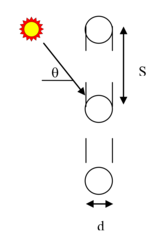
\includegraphics[width=0.9\textwidth, height=0.9\textheight, keepaspectratio=true]{media/image048.png}
\caption{Geometry used for insect screen analysis \protect \label{fig:geometry-used-for-insect-screen-analysis}}
\end{figure}

The formulation of the model, assumption and correlations used to calculate effective solar and longwave properties of insect screens are described in the Engineering Reference.

\subsubsection{Inputs}\label{inputs-29-001}

\paragraph{Field: Name}\label{field-name-23-003}

Name of the insect screen. It is referenced as an outside layer in an equivalent layer window construction.

\paragraph{Field: Screen Beam-Beam Solar Transmittance}\label{field-screen-beam-beam-solar-transmittance}

This value is the beam-beam transmittance of the screen material at normal incidence. This value is the same as the screen openness area fraction.~ This value can be autocalculated from the wire spacing and wire diameter. It is the same for both sides of the screen. The minimum value is 0.0, and maximum value is less than 1.0.

\paragraph{Field: Screen Beam-Diffuse Solar Transmittance}\label{field-screen-beam-diffuse-solar-transmittance}

This value is the beam-diffuse solar transmittance of the screen material at normal incidence averaged over the entire spectrum of solar radiation. Assumed to be the same for both sides of the screen. The minimum value is 0.0, and the maximum value is less than 1.0.

\paragraph{Field: Screen Beam-Diffuse Solar Reflectance}\label{field-screen-beam-diffuse-solar-reflectance}

This value is the beam-diffuse solar reflectance of the screen material at normal incidence averaged over the entire spectrum of solar radiation. Assumed to be the same for both sides of the screen. The minimum value is 0.0, and the maximum value is less than 1.0.

\paragraph{Field: Screen Beam-Beam Visible Transmittance}\label{field-screen-beam-beam-visible-transmittance}

This value is the beam-beam visible transmittance of the screen material at normal incidence averaged over the visible spectrum range of solar radiation.~ Assumed to be the same for both sides of the screen. The minimum value is 0.0, and maximum value is less than 1.0. This input input field is not used currently.

\paragraph{Field: Screen Beam-Diffuse Visible Transmittance}\label{field-screen-beam-diffuse-visible-transmittance}

This value is the beam-diffuse visible reflectance of the screen material at normal incidence averaged over the visible spectrum range of solar radiation. Assumed to be the same for both sides of the screen. The minimum value is 0.0, and the maximum value is less than 1.0. This input input field is not used currently.

\paragraph{Field: Screen Beam-Diffuse Visible Reflectance}\label{field-screen-beam-diffuse-visible-reflectance}

This value is the beam-diffuse visible reflectance of the screen material at normal incidence averaged over the visible spectrum range of solar radiation. Assumed to be the same for both sides of the screen. The minimum value is 0.0, and the maximum value is less than 1.0. This input input field is not used currently.

\paragraph{Field: Screen Infrared Transmittance}\label{field-screen-infrared-transmittance}

This value is the long-wave hemispherical transmittance of the the screen material. Assumed to be the same for both sides of the screen material. The minimum value is 0.0, the maximum value is less than 1.0.~ The default value is 0.02

\paragraph{Field: Screen Infrared Emissivity}\label{field-screen-infrared-emissivity}

This value is the long-wave hemispherical emissivity of the screen material. Assumed to be the same for both sides of the screen material. The minimum value is 0.0, the maximum value is less than 1.0. The default value is 0.93.

\paragraph{Field: Screen Wire Spacing}\label{field-screen-wire-spacing}

The spacing, S (m), of the screen material is the distance from the center of one strand of screen to the center of the adjacent one. The spacing of the screen material is assumed to be the same in both directions (e.g., vertical and horizontal). This input value must be greater than the non-zero screen material diameter. If the spacing is different in the two directions, use the average of the two values. Default value is 0.0025m.

\paragraph{Field: Screen Wire Diameter}\label{field-screen-wire-diameter}

The diameter, D (m), of individual strands or wires of the screen material. The screen material diameter is assumed to be the same in both directions (e.g., vertical and horizontal). This input value must be greater than 0 and less than the screen wire spacing. If the diameter is different in the two directions, use the average of the two values. Default value is 0.005m.

An IDF example for this object, is shown below:

\begin{lstlisting}

WindowMaterial:Screen:EquivalentLayer,
    INSCRN,                !- Name
    0.763,                 !- Screen Beam-Beam Solar Transmittance
    0.052,                 !- Screen Beam-Diffuse Solar Transmittance
    0.076,                 !- Screen Beam-Diffuse Solar Reflectance
    0.0,                   !- Screen Beam-Beam Visible Transmittance
    0.0,                   !- Screen Beam-Diffuse Visible Transmittance
    0.0,                   !- Screen Beam-Diffuse Visible Reflectance
    0.0,                   !- Screen Infrared Transmittance
    0.84,                  !- Screen Infrared Emissivity
    0.025,                 !- Screen Wire Spacing
    0.005;                 !- Screen Wire Diameter
\end{lstlisting}

\subsection{WindowMaterial:Glazing:EquivalentLayer}\label{windowmaterialglazingequivalentlayer}

Glass material properties for equivalent layer window model.~ Uses transmittance/reflectance input method.~ For exterior windows, ``front side'' is the side of the glass closest to the outside air and ``back side'' is the side closest to the zone the window is defined in. For interzone windows, ``front side'' is the side closest to the zone adjacent to the zone the window is defined in and ``back side'' is the side closest to the zone the window is defined in. The equivalent layer window glazing model does not support \hyperref[windowpropertyshadingcontrol]{WindowShadingControl}.

\subsubsection{Inputs}\label{inputs-30-001}

\paragraph{Field: Name}\label{field-name-24-002}

The name of the glass layer. It corresponds to a layer in an equivalent layer window construction.

\paragraph{Field: Optical Data Type}\label{field-optical-data-type-1}

Valid values for this field are SpectralAverage, or Spectral. If Optical Data Type = SpectralAverage, the values you enter for solar transmittance and reflectance are assumed to be averaged over the solar spectrum, and the values you enter for visible transmittance and reflectance are assumed to be averaged over the solar spectrum and weighted by the response of~ the human eye. SpectralAverage is the default. Spectral data input is not supported now.

\paragraph{Field: Window Glass Spectral Data Set Name}\label{field-window-glass-spectral-data-set-name-0}

This input field is not used currently.

\paragraph{Field: Front Side Beam-Beam Solar Transmittance}\label{field-front-side-beam-beam-solar-transmittance}

This value is the front side beam-beam solar transmittance of the glazing at normal incidence averaged over the entire spectrum of solar radiation.~ Used only when Optical Data Type = SpectralAverage.~ The minimum value is 0.0, and the maximum value is less than 1.0.

\paragraph{Field: Back Side Beam-Beam Solar Transmittance}\label{field-back-side-beam-beam-solar-transmittance}

This value is the back side beam-beam solar transmittance of the glazing at normal incidence averaged over the entire spectrum of solar radiation.~ Used only when Optical Data Type = SpectralAverage.~ The minimum value is 0.0, and the maximum value is less than 1.0.

\paragraph{Field: Front Side Beam-Beam Solar Reflectance}\label{field-front-side-beam-beam-solar-reflectance}

This value is the front side beam-beam solar reflectance of the glazing at normal incidence averaged over the entire spectrum of solar radiation.~ Used only when Optical Data Type = SpectralAverage.~ The minimum value is 0.0, and the maximum value is less than 1.0.

\paragraph{Field: Back Side Beam-Beam Solar Reflectance}\label{field-back-side-beam-beam-solar-reflectance}

This value is the back side beam-beam solar reflectance of the glazing at normal incidence averaged over the entire spectrum of solar radiation.~ Used only when Optical Data Type = SpectralAverage.~ The minimum value is 0.0, and the maximum value is less than 1.0.

\paragraph{Field: Front Side Beam-Beam Visible Transmittance}\label{field-front-side-beam-beam-visible-transmittance}

This value is the front side beam-beam visible transmittance of the glazing at normal incidence averaged over the visible spectrum range of solar radiation.~ Used only when Optical Data Type = SpectralAverage.~ The minimum value is 0.0, and the maximum value is less than 1.0.

\paragraph{Field: Back Side Beam-Beam Visible Transmittance}\label{field-back-side-beam-beam-visible-transmittance}

This value is the back side beam-beam visible transmittance of the glazing at normal incidence averaged over the visible spectrum range of solar radiation.~ Used only when Optical Data Type = SpectralAverage.~ The minimum value is 0.0, and the maximum value is less than 1.0.

\paragraph{Field: Front Side Beam-Beam Visible Reflectance}\label{field-front-side-beam-beam-visible-reflectance}

This value is the front side beam-beam visible reflectance of the glazing at normal incidence averaged over the visible spectrum range of solar radiation.~ Used only when Optical Data Type = SpectralAverage.~ The minimum value is 0.0, and the maximum value is less than 1.0.

\paragraph{Field: Back Side Beam-Beam Visible Reflectance}\label{field-back-side-beam-beam-visible-reflectance}

This value is the back side beam-beam visible reflectance of the glazing at normal incidence averaged over the visible spectrum range of solar radiation.~ Used only when Optical Data Type = SpectralAverage.~ The minimum value is 0.0, and the maximum value is less than 1.0.

\paragraph{Field: Front Side Beam-Diffuse Solar Transmittance}\label{field-front-side-beam-diffuse-solar-transmittance}

This value is the front side beam-diffuse solar transmittance of the glazing at normal incidence averaged over the entire spectrum of solar radiation.~ Used only when Optical Data Type = SpectralAverage.~ For clear glazing the beam-diffuse transmittance is zero. The minimum value is 0.0, and the maximum value is less than 1.0. Default value is 0.0.

\paragraph{Field: Back Side Beam-Diffuse Solar Transmittance}\label{field-back-side-beam-diffuse-solar-transmittance}

This value is the back side beam-diffuse solar transmittance of the glazing at normal incidence averaged over the entire spectrum of solar radiation.~ Used only when Optical Data Type = SpectralAverage.~ For clear glazing the beam-diffuse solar transmittance is zero. The minimum value is 0.0, and the maximum value is less than 1.0. Default value is 0.0.

\paragraph{Field: Front Side Beam-Diffuse Solar Reflectance}\label{field-front-side-beam-diffuse-solar-reflectance}

This value is the front side beam-diffuse solar reflectance of the glazing at normal incidence averaged over the entire spectrum of solar radiation.~ Used only when Optical Data Type = SpectralAverage.~ The minimum value is 0.0, and the maximum value is less than 1.0. Default value is 0.0.

\paragraph{Field: Back Side Beam-Diffuse Solar Reflectance}\label{field-back-side-beam-diffuse-solar-reflectance}

This value is the back side beam-diffuse solar reflectance of the glazing at normal incidence averaged over the entire spectrum of solar radiation.~ Used only when Optical Data Type = SpectralAverage.~ The minimum value is 0.0, and the maximum value is less than 1.0. Default value is 0.0.

\paragraph{Field: Front Side Beam-Diffuse Visible Transmittance}\label{field-front-side-beam-diffuse-visible-transmittance}

This value is the front side beam-diffuse visible transmittance of the glazing at normal incidence averaged over the visible spectrum range of solar radiation.~ Used only when Optical Data Type = SpectralAverage.~ For clear glazing the beam-diffuse visible transmittance is zero. The minimum value is 0.0, and the maximum value is less than 1.0. Default value is 0.0.~ This input field is not used currently.

\paragraph{Field: Back Side Beam-Diffuse Visible Transmittance}\label{field-back-side-beam-diffuse-visible-transmittance}

This value is the back side beam-diffuse visible transmittance of the glazing at normal incidence averaged over the visible spectrum range of solar radiation.~ Used only when Optical Data Type = SpectralAverage.~ For clear glazing the beam-diffuse visible transmittance is zero. The minimum value is 0.0, and the maximum value is less than 1.0. Default value is 0.0.~ This input field is not used currently.

\paragraph{Field: Front Side Beam-Diffuse Visible Reflectance}\label{field-front-side-beam-diffuse-visible-reflectance}

This value is the front side beam-diffuse visible reflectance of the glazing at normal incidence averaged over the visible spectrum range of solar radiation.~ Used only when Optical Data Type = SpectralAverage.~ The minimum value is 0.0, and the maximum value is less than 1.0. Default value is 0.0. This input field is not used currently.

\paragraph{Field: Back Side Beam-Diffuse Visible Reflectance}\label{field-back-side-beam-diffuse-visible-reflectance}

This value is the back side beam-diffuse visible reflectance of the glazing at normal incidence averaged over the visible spectrum range of solar radiation.~ Used only when Optical Data Type = SpectralAverage.~ The minimum value is 0.0, and the maximum value is less than 1.0. Default value is 0.0. This input field is not used currently.

\paragraph{Field: Diffuse-Diffuse Solar Transmittance}\label{field-diffuse-diffuse-solar-transmittance}

This value is the diffuse-diffuse solar transmittance of the glazing averaged over the entire spectrum of solar radiation.~ Used only when Optical Data Type = SpectralAverage. The diffuse-diffuse transmittance is assumed to be the same for both sides of the glazing.~ EnergyPlus automatically estimates the diffuse-diffuse solar transmittance from other inputs. If this input field is specified as ``Autocalculate'', then the calculated transmittance will be used. The minimum value is 0.0, and the maximum value is less than 1.0.

\paragraph{Field: Front Side Diffuse-Diffuse Solar Reflectance}\label{field-front-side-diffuse-diffuse-solar-reflectance}

This value is the front side diffuse-diffuse solar reflectance of the glazing averaged over the entire spectrum of solar radiation.~ Used only when Optical Data Type = SpectralAverage. EnergyPlus automatically estimates the diffuse-diffuse reflectance from other inputs. If this input field is specified as ``Autocalculate'', then the calculated reflectance will be used. The minimum value is 0.0, and the maximum value is less than 1.0.

\paragraph{Field: Back Side Diffuse-Diffuse Solar Reflectance}\label{field-back-side-diffuse-diffuse-solar-reflectance}

This value is the back side diffuse-diffuse solar reflectance of the glazing averaged over the entire spectrum of solar radiation.~ Used only when Optical Data Type = SpectralAverage. EnergyPlus automatically estimates the diffuse-diffuse reflectance from other inputs. If this input field is specified as ``Autocalculate'', then the calculated reflectance will be used. The minimum value is 0.0, and the maximum value is less than 1.0.

\paragraph{Field: Diffuse-Diffuse Visible Solar Transmittance}\label{field-diffuse-diffuse-visible-solar-transmittance}

This value is the diffuse-diffuse visible transmittance of the glazing averaged over the visible spectrum range of solar radiation.~ Used only when Optical Data Type = SpectralAverage. The diffuse-diffuse visible transmittance is assumed to be the same for both sides of the glazing.~ If this input field is specified as ``Autocalculate'', then the calculated transmittance will be used. The minimum value is 0.0, and the maximum value is less than 1.0. This input field is not used currently.

\paragraph{Field: Front Side Diffuse-Diffuse Visible Reflectance}\label{field-front-side-diffuse-diffuse-visible-reflectance}

This value is the front side diffuse-diffuse visible reflectance of the glazing averaged over the visible spectrum range of solar radiation.~ Used only when Optical Data Type = SpectralAverage. EnergyPlus automatically estimates the front side diffuse-diffuse visible reflectance from front side beam-beam visible reflectance at normal incidence specified above. If this input field is specified as ``Autocalculate'', then the calculated reflectance will be used. The minimum value is 0.0, and the maximum value is less than 1.0. This input field is not used currently.

\paragraph{Field: Back Side Diffuse-Diffuse Visible Reflectance}\label{field-back-side-diffuse-diffuse-visible-reflectance}

This value is the back side diffuse-diffuse visible reflectance of the glazing averaged over the visible spectrum range of solar radiation.~ Used only when Optical Data Type = SpectralAverage. EnergyPlus automatically estimates the back side diffuse-diffuse visible reflectance from back side beam-beam visible reflectance at normal incidence specified above. If this input field is specified as ``Autocalculate'', then the calculated reflectance will be used. The minimum value is 0.0, and the maximum value is less than 1.0. This input field is not used currently.

\paragraph{Field: Infrared Transmittance (applies to front and back)}\label{field-infrared-transmittance-applies-to-front-and-back}

This value is the long-wave hemispherical transmittance of the glazing. Assumed to be the same for both sides of the glazing. The minimum value is 0.0, the maximum value is less than 1.0.~ The default value is 0.0.

\paragraph{Field: Front Side Infrared Emissivity}\label{field-front-side-infrared-emissivity}

This value is the front side long-wave hemispherical emissivity of the glazing. The minimum value is 0.0, the maximum value is less than 1.0.~ The default value is 0.84.

\paragraph{Field: Back Side Infrared Emissivity}\label{field-back-side-infrared-emissivity}

This value is the back side long-wave hemispherical emissivity of the glazing. The minimum value is 0.0, the maximum value is less than 1.0.~ The default value is 0.84.

\paragraph{Field: Thermal Resistance}\label{field-thermal-resistance-equivglazing}

This field is used to enter the thermal resistance (R-value) of the material layer. Units for this parameter are (m\(^{2}\)-K)/W. Thermal resistance must be greater than zero. The default value is 0.158 which is roughly equivalent to a single layer of 1/4" glass. This field is only used if this equivalent layer of glazing is being referenced for movable insulation.

An IDF example for this object, is shown below:

\begin{lstlisting}

WindowMaterial:Glazing:EquivalentLayer,
    GLZCLR,                  !- Name
    SpectralAverage,         !- Optical Data Type
    ,                        !- Window Glass Spectral Data Set Name
    0.83,                    !- Front Side Beam-Beam Solar Transmittance
    0.83,                    !- Back Side Beam-Beam Solar Transmittance
    0.08,                    !- Front Side Beam-Beam Solar Reflectance
    0.08,                    !- Back Side Beam-Beam Solar Reflectance
    0.0,                     !- Front Side Beam-Beam Visible Transmittance
    0.0,                     !- Back Side Beam-Beam Visible Transmittance
    0.0,                     !- Front Side Beam-Beam Visible Reflectance
    0.0,                     !- Back Side Beam-Beam Visible Reflectance
    0.0,                     !- Front Side Beam-Diffuse Solar Transmittance
    0.0,                     !- Back Side Beam-Diffuse Solar Transmittance
    0.0,                     !- Front Side Beam-Diffuse Solar Reflectance
    0.0,                     !- Back Side Beam-Diffuse Solar Reflectance
    0.0,                     !- Front Side Beam-Diffuse Visible Transmittance
    0.0,                     !- Back Side Beam-Diffuse Visible Transmittance
    0.0,                     !- Front Side Beam-Diffuse Visible Reflectance
    0.0,                     !- Back Side Beam-Diffuse Visible Reflectance
    0.76,                    !- Diffuse-Diffuse Solar Transmittance
    0.14,                    !- Front Side Diffuse-Diffuse Solar Reflectance
    0.14,                    !- Back Side Diffuse-Diffuse Solar Reflectance
    0.0,                     !- Diffuse-Diffuse Visible Transmittance
    0.0,                     !- Front Side Diffuse-Diffuse Visible Reflectance
    0.0,                     !- Back Side Diffuse-Diffuse Visible Reflectance
    0.0,                     !- Infrared Transmittance
    0.84,                    !- Front Side Infrared Emissivity
    0.84,                    !- Back Side Infrared Emissivity
    0.158;                   !- Thermal Resistance (used for movable insulation only)
\end{lstlisting}

\subsection{WindowMaterial:Gap:EquivalentLayer}\label{windowmaterialgapequivalentlayer}

This object is used in windows equivalent layer construction object and specifies the properties of the gap between the layers in multi-layer equivalent layer window object. There is an EnergyPlus Reference Data Set for Material:WindowGas that contains several types of gas. This object uses the gas types: Air, Argon, Xenon, Crypton, and Custom.~ For Custom gas type users are required to entering the thermophicial properties.

\subsubsection{Inputs}\label{inputs-31-001}

\paragraph{Field: Name}\label{field-name-25-002}

The name of the gap. It refers to a layer in a window construction equivalent layer.

\paragraph{Field: Gas Type}\label{field-gas-type-1}

The type of gas. The choices allowed are AIR, ARGON, XENON, KRYPTON, or CUSTOM.

\paragraph{Field: Thickness}\label{field-thickness-8}

The thickness (m) of the gap layer.

\paragraph{Field: Gap Vent Type}\label{field-gap-vent-type}

This input field contains the valid key choice for gap vent type.~ The valid vent types are: Sealed, VentedIndoor, and VentedOutdoor.~ Sealed means the gap is enclosed and gas tight, i.e., no venting to indoor or outdoor environment. The gap types ``VentedIndoor'' and ``VentedOutdoor'' are used with gas type ``Air'' only. VentedIndoor means the air in the gap is naturally vented to indoor environment, and~ VentedOutdoor means the air in the gap is naturally vented to the outdoor environment.

\paragraph{Properties for Custom Gas Types}\label{properties-for-custom-gas-types-1}

The following entries are used only if Gas Type = Custom. The A, B and C coefficients are those in the following expression that gives a property value as a function of temperature in degrees K:

\begin{equation}
Property = Coef{f_A} + Coef{f_B} \times Temperatur{e_K} + Coef{f_C} \times Temperature_K^2
\end{equation}

\paragraph{Field: Conductivity Coefficient A}\label{field-conductivity-coefficient-a-1}

The A coefficient for gas conductivity (W/m-K). Used only if Gas Type = Custom.

\paragraph{Field: Conductivity Coefficient B}\label{field-conductivity-coefficient-b-1}

The B coefficient for gas conductivity (W/m-K\(^{2}\)). Used only if Gas Type = Custom.

\paragraph{Field: Conductivity Coefficient C}\label{field-conductivity-coefficient-c-1}

The C coefficient for gas conductivity (W/m-K\(^{3}\)).~ Used only if Gas Type = Custom.

\paragraph{Field: Viscosity Coefficient A}\label{field-viscosity-coefficient-a-1}

The A coefficient for gas viscosity (kg/m-s). Used only if Gas Type = Custom.

\paragraph{Field: Viscosity Coefficient B}\label{field-viscosity-coefficient-b-1}

The B coefficient for gas viscosity (kg/m-s-K). Used only if Gas Type = Custom.

\paragraph{Field: Viscosity Coefficient C}\label{field-viscosity-coefficient-c-1}

The C coefficient for gas viscosity (kg/m-s-K\(^{2}\)).~ Used only if Gas Type = Custom.

\paragraph{Field: Specific Heat Coefficient A}\label{field-specific-heat-coefficient-a-1}

The A coefficient for gas specific heat (J/kg-K). Used only if Gas Type = Custom.

\paragraph{Field: Specific Heat Coefficient B}\label{field-specific-heat-coefficient-b-1}

The B coefficient for gas specific heat (J/kg-K\(^{2}\)). Used only if Gas Type = Custom.

\paragraph{Field: Specific Heat Coefficient C}\label{field-specific-heat-coefficient-c-1}

The C coefficient for gas specific heat (J/kg-K\(^{2}\)).~ Used only if Gas Type = Custom.

\paragraph{Field: Specific Heat Ratio}\label{field-specific-heat-ratio-2}

The specific heat ratio for gas.~ Used only if Gas Type = Custom.

\paragraph{Field: Molecular Weight}\label{field-molecular-weight-1}

The molecular weight for gas.~ The molecular weight is the mass of 1 mol of the substance.~ This has a numerical value which is the average molecular mass of the molecules in the substance multiplied by Avogadro's constant. (kg/kmol) (Shown in the IDD as g/mol for consistency)

\paragraph{Field: Specific Heat Ratio}\label{field-specific-heat-ratio-3}

The specific heat ratio for gas.~ The specific heat ratio of a gas is the ratio of the specific heat at constant pressure, to the specific heat at constant volume.~ Used only if Gas Type = Custom.

An IDF example for this object, is shown below:

\begin{lstlisting}

WindowMaterial:Gap:EquivalentLayer,
    Custom CO2 Sealed 12mm,    !- Name
    CUSTOM,                    !- Gas Type
    0.0120,                    !- Thickness {m}
    Sealed,                    !- Gap Vent Type
   -5.8181E-3,                 !- Conductivity Coefficient A {W/m-K}
    7.4714E-5,                 !- Conductivity Coefficient B {W/m-K2}
    0.0,                       !- Conductivity Coefficient C {W/m-K3}
    8.5571E-7,                 !- Viscosity Coefficient A {kg/m-s}
    4.7143E-8,                 !- Viscosity Coefficient B {kg/m-s-K}
    0.0,                       !- Viscosity Coefficient C {kg/m-s-K2}
    5.76903E2,                 !- Specific Heat Coefficient A {J/kg-K}
    9.18088E-2,                !- Specific Heat Coefficient B {J/kg-K2}
    0.0,                       !- Specific Heat Coefficient C {J/kg-K3}
    44.01;                     !- Molecular Weight {g/mol}
\end{lstlisting}

\subsection{Material:RoofVegetation}\label{materialroofvegetation}

This definition must be used in order to simulate the green roof (ecoroof) model. The material becomes the outside layer in a green roof construction (see example below). In the initial release of the green roof model, only one material may be used as a green roof layer though, of course, several constructions using that material may be used. In addition, the model works only with the ConductionTransferFunction heat balance solution algorithm. This model was developed for low-sloped exterior surfaces (roofs). It is not recommended for high-sloped exterior surfaces (e.g., walls).

\subsubsection{Inputs}\label{inputs-32-000}

\paragraph{Field: Name}\label{field-name-26-002}

This field is a unique reference name that the user assigns to a particular ecoroof material. This name can then be referred to by other input data.

\paragraph{Field: Height of Plants}\label{field-height-of-plants}

This field defines the height of plants in units of meters. This field is limited to values in the range 0.005 \textless{} Height \textless{} 1.00 m. Default is .2 m.

\paragraph{Field: Leaf Area Index}\label{field-leaf-area-index}

This is the projected leaf area per unit area of soil surface. This field is dimensionless and is limited to values in the range of 0.001 \textless{} LAI \textless{} 5.0. Default is 1.0. At the present time the fraction vegetation cover is calculated directly from LAI (Leaf Area Index) using an empirical relation. The user may find it necessary to increase the specified value of LAI in order to represent high fractional coverage of the surface by vegetation.

\paragraph{Field: Leaf Reflectivity}\label{field-leaf-reflectivity}

This field represents the fraction of incident solar radiation that is reflected by the individual leaf surfaces (albedo). Solar radiation includes the visible spectrum as well as infrared and ultraviolet wavelengths. Values for this field must be between 0.05 and 0.5. Default is .22. Typical values are .18 to .25.

\paragraph{Field: Leaf Emissivity}\label{field-leaf-emissivity}

This field is the ratio of thermal radiation emitted from leaf surfaces to that emitted by an ideal black body at the same temperature. This parameter is used when calculating the long wavelength radiant exchange at the leaf surfaces. Values for this field must be between 0.8 and 1.0 (with 1.0 representing ``black body'' conditions). Default is .95.

\paragraph{Field: Minimum Stomatal Resistance}\label{field-minimum-stomatal-resistance}

This field represents the resistance of the plants to moisture transport. It has units of s/m. Plants with low values of stomatal resistance will result in higher evapotranspiration rates than plants with high resistance. Values for this field must be in the range of 50.0 to 300.0. Default is 180.

\paragraph{Field: Soil Layer Name}\label{field-soil-layer-name}

This field is a unique reference name that the user assigns to the soil layer for a particular ecoroof. This name can then be referred to by other input data. Default is \textbf{Green Roof Soil}.

\paragraph{Field: Roughness}\label{field-roughness-2}

This alpha field defines the relative roughness of a particular material layer. This parameter only influences the convection coefficients, more specifically the exterior convection coefficient. A keyword is expected in this field with the options being ``VeryRough'', ``Rough'', ``MediumRough'', ``MediumSmooth'', ``Smooth'', and ``VerySmooth'' in order of roughest to smoothest options. Default is MediumRough.

\paragraph{Field: Thickness}\label{field-thickness-9}

This field characterizes the thickness of the material layer in meters. This should be the dimension of the layer in the direction perpendicular to the main path of heat conduction. This value must be a positive number. Depths of 0.10 m (4 inches) and 0.15 m (6 inches) are common. Default if this field is left blank is 0.1. Maximum is 0.7 m. Must be greater than 0.05 m.

\paragraph{Field: Conductivity of Dry Soil}\label{field-conductivity-of-dry-soil}

This field is used to enter the thermal conductivity of the material layer. Units for this parameter are W/(m-K). Thermal conductivity must be greater than zero. Typical soils have values from 0.3 to 0.5. The minimum is 0.2, the default is 0.35, and the maximum is 1.5.

\paragraph{Field: Density of Dry Soil}\label{field-density-of-dry-soil}

This field is used to enter the density of the material layer in units of kg/m\(^{3}\). Density must be a positive quantity. Typical soils range from 400 to 1000 (dry to wet). Minimum is 300, maximum is 2000 and default if field is left blank is 1100.

\paragraph{Field: Specific Heat of Dry Soil}\label{field-specific-heat-of-dry-soil}

This field represents the specific heat of the material layer in units of J/(kg-K). Note that these units are most likely different than those reported in textbooks and references which tend to use kJ/(kg-K) or J/(g-K). They were chosen for internal consistency within EnergyPlus. Only positive values of specific heat are allowed.

\paragraph{Field: Thermal Absorptance}\label{field-thermal-absorptance-2}

The thermal absorptance field in the Material input syntax represents the fraction of incident long wavelength (>2.5 microns) radiation that is absorbed by the material. This parameter is used when calculating the long wavelength radiant exchange between various surfaces and affects the surface heat balances (both inside and outside as appropriate). For long wavelength radiant exchange, thermal emissivity and thermal emittance are equal to thermal absorptance. Values for this field must be between 0.0 and 1.0 (with 1.0 representing ``black body'' conditions). Typical values are from 0.9 to 0.98. The default value for this field is 0.9.

\paragraph{Field: Solar Absorptance}\label{field-solar-absorptance-2}

The solar absorptance field in the Material input syntax represents the fraction of incident~ solar radiation that is absorbed by the material. Solar radiation (0.3 to 2.537 $\mu{}m$) includes the visible spectrum as well as infrared and ultraviolet wavelengths. This parameter is used when calculating the amount of incident solar radiation absorbed by various surfaces and affects the surface heat balances (both inside and outside as appropriate). If solar reflectance (or reflectivity) data is available, then absorptance is equal to 1.0 minus reflectance (for opaque materials). Values for this field must be between 0.0 and 1.0. Typical values are from .6 to .85. The default value for this field is 0.7.

\paragraph{Field: Visible Absorptance}\label{field-visible-absorptance-2}

The visible absorptance field in the Material input syntax represents the fraction of incident visible wavelength radiation that is absorbed by the material. Visible wavelength radiation ( 0.37 to 0.78 $\mu{}m$ weighted by photopic response) is slightly different than solar radiation in that the visible band of wavelengths is much more narrow while solar radiation includes the visible spectrum as well as infrared and ultraviolet wavelengths. This parameter is used when calculating the amount of incident visible radiation absorbed by various surfaces and affects the surface heat balances (both inside and outside as appropriate) as well as the daylighting calculations. If visible reflectance (or reflectivity) data is available, then absorptance is equal to 1.0 minus reflectance (for opaque materials). Values for this field must be between 0.5 and 1.0. The default value for this field is 0.75.

\paragraph{Field: Saturation Volumetric Moisture Content of the Soil Layer}\label{field-saturation-volumetric-moisture-content-of-the-soil-layer}

The field allows for user input of the saturation moisture content of the soil layer. Maximum moisture content is typically less than .5. Range is {[}.1,.5{]} with the default being .3.

\paragraph{Field: Residual Volumetric Moisture Content of the Soil Layer}\label{field-residual-volumetric-moisture-content-of-the-soil-layer}

The field allows for user input of the residual moisture content of the soil layer. Default is 0.01, range is {[}0.01, 0.1{]}.

\paragraph{Field: Initial Volumetric Moisture Content of the Soil Layer}\label{field-initial-volumetric-moisture-content-of-the-soil-layer}

The field allows for user input of the initial moisture content of the soil layer. Range is (0.05, 0.5{]} with the default being 0.1.

\paragraph{Field: Moisture Diffusion Calculation Method}\label{field-moisture-diffusion-calculation-method}

The field allows for two models to be selected: \textbf{Simple} or \textbf{Advanced}. EnergyPlus Currently supports only the \textbf{Simple} \textit{Moisture Diffusion Calculation Method}.

\textbf{Simple} is the original Ecoroof model - based on a constant diffusion of moisture through the soil.~ This model starts with the soil in two layers.~ Every time the soil properties update is called, it will look at the two soils moisture layers and asses which layer has more moisture in it. It then takes moisture from the higher moisture layer and redistributes it to the lower moisture layer at a constant rate.

\textbf{Advanced} is the later Ecoroof model. The model requires higher number of timesteps in hour for the simulation with a recommended value of 20. This moisture transport model is based on a project which looked at the way moisture transports through soil.~ It uses a finite difference method to divide the soil into layers (nodes). It redistributes the soil moisture according the model described in:

Marcel G Schaap and Martinus Th. van Genuchten, 2006, `A modified Maulem-van Genuchten Formulation for Improved Description of the Hydraulic Conductivity Near Saturation', Vadose Zone Journal 5 (1), p 27-34. However, currently \textbf{Advanced} \textit{Moisture Diffusion Calculation Method} is not supported in EnergyPlus.

An IDF example:

\begin{lstlisting}

Material:RoofVegetation,
      BaseEco,                 !- Name
      0.5,                     !- Height of Plants {m}
      5,                       !- Leaf Area Index {dimensionless}
      0.2,                     !- Leaf Reflectivity {dimensionless}
      0.95,                    !- Leaf Emissivity
      180,                     !- Minimum Stomatal Resistance {s/m}
      EcoRoofSoil,             !- Soil Layer Name
      MediumSmooth,            !- Roughness
      0.18,                    !- Thickness {m}
      0.4,                     !- Conductivity of Dry Soil {W/m-K}
      641,                     !- Density of Dry Soil {kg/m3}
      1100,                    !- Specific Heat of Dry Soil {J/kg-K}
      0.95,                    !- Thermal Absorptance
      0.8,                     !- Solar Absorptance
      0.7,                     !- Visible Absorptance
      0.4,                     !- Saturation Volumetric Moisture Content of the Soil Layer
      0.01,                    !- Residual Volumetric Moisture Content of the Soil Layer
      0.2,                     !- Initial Volumetric Moisture Content of the Soil Layer
      Simple;                  !- Moisture Diffusion Calculation Method


    Material:RoofVegetation,
      LowLAI,                  !- Name
      0.5,                     !- Height of Plants {m}
      0.5,                     !- Leaf Area Index {dimensionless}
      0.2,                     !- Leaf Reflectivity {dimensionless}
      0.95,                    !- Leaf Emissivity
      180,                     !- Minimum Stomatal Resistance {s/m}
      EcoRoofSoil,             !- Soil Layer Name
      MediumSmooth,            !- Roughness
      0.18,                    !- Thickness {m}
      0.4,                     !- Conductivity of Dry Soil {W/m-K}
      641,                     !- Density of Dry Soil {kg/m3}
      1100,                    !- Specific Heat of Dry Soil {J/kg-K}
      0.95,                    !- Thermal Absorptance
      0.8,                     !- Solar Absorptance
      0.7,                     !- Visible Absorptance
      0.4,                     !- Saturation Volumetric Moisture Content of the Soil Layer
      0.01,                    !- Residual Volumetric Moisture Content of the Soil Layer
      0.2,                     !- Initial Volumetric Moisture Content of the Soil Layer
      Simple;                 !- Moisture Diffusion Calculation Method
\end{lstlisting}

And construction using the ecoroof material:

\begin{lstlisting}

Construction,
      ASHRAE 90.1-2004_Sec 5.5-2_Roof,  !- Name
      BaseEco,                 !- Outside Layer
      ASHRAE 90.1-2004_Sec 5.5-2_Roof Insulation_1,  !- Layer \#2
      ASHRAE 90.1-2004_Sec 5.5-2_MAT-METAL;  !- Layer \#3
\end{lstlisting}

\subsubsection{Ecoroof / RoofVegetation outputs}\label{ecoroof-roofvegetation-outputs}

The following outputs are available for the Roof Vegetation surface.

\begin{itemize}
\item
  Zone,Average,Green Roof Soil Temperature {[}C{]}
\item
  Zone,Average,Green Roof Vegetation Temperature {[}C{]}
\item
  Zone,Average,Green Roof Soil Root Moisture Ratio {[]}
\item
  Zone,Average,Green Roof Soil Near Surface Moisture Ratio {[]}
\item
  Zone,Average,Green Roof Soil Sensible Heat Transfer Rate per Area {[}W/m2{]}
\item
  Zone,Average,Green Roof Vegetation Sensible Heat Transfer Rate per Area {[}W/m2{]}
\item
  Zone,Average,Green Roof Vegetation Moisture Transfer Rate {[}m/s{]}
\item
  Zone,Average,Green Roof Soil Moisture Transfer Rate {[}m/s{]}
\item
  Zone,Average,Green Roof Vegetation Latent Heat Transfer Rate per Area {[}W/m2{]}
\item
  Zone,Average,Green Roof Soil Latent Heat Transfer Rate per Area {[}W/m2{]}
\item
  Zone,Sum,Green Roof Cumulative Precipitation Depth {[}m{]}
\item
  Zone,Sum,Green Roof Cumulative Irrigation Depth {[}m{]}
\item
  Zone,Sum,Green Roof Cumulative Runoff Depth {[}m{]}
\item
  Zone,Sum,Green Roof Cumulative Evapotranspiration Depth {[}m{]}
\item
  Zone,Sum,Green Roof Current Precipitation Depth {[}m{]}
\item
  Zone,Sum,Green Roof Current Irrigation Depth {[}m{]}
\item
  Zone,Sum,Green Roof Current Runoff Depth {[}m{]}
\item
  Zone,Sum,Green Roof Current Evapotranspiration Depth {[}m{]}
\end{itemize}

\paragraph{Green Roof Soil Temperature {[}C{]}}\label{green-roof-soil-temperature-c}

Temperature of the Soil layer temperature in C. Note that \hyperref[surface-outside-face-temperature-c]{Surface Outside Face Temperature} of Roof, one of the surface output variables, is the temperature at the interface between the soil and the next material layer.

\paragraph{Green Roof Vegetation Temperature {[}C{]}}\label{green-roof-vegetation-temperature-c}

Temperature of the Vegetation layer temperature in degree Celsius ($^\circ$C).

\paragraph{Green Roof Soil Root Moisture Ratio {[]}}\label{green-roof-soil-root-moisture-ratio}

Mean value of root moisture (m\(^{3}\)/m\(^{3}\))

\paragraph{Green Roof Soil Near Surface Moisture Ratio {[]}}\label{green-roof-soil-near-surface-moisture-ratio}

The moisture content in the soil near the surface (m\(^{3}\)/m\(^{3}\))

\paragraph{Green Roof Soil Sensible Heat Transfer Rate per Area {[}W/m2{]}}\label{green-roof-soil-sensible-heat-transfer-rate-per-area-wm2}

Sensible heat flux to ground (W/m\(^{2}\))

\paragraph{Green Roof Vegetation Sensible Heat Transfer Rate per Area {[}W/m2{]}}\label{green-roof-vegetation-sensible-heat-transfer-rate-per-area-wm2}

Sensible heat transfer to foliage (W/m\(^{2}\))

\paragraph{Green Roof Vegetation Moisture Transfer Rate {[}m/s{]}}\label{green-roof-vegetation-moisture-transfer-rate-ms}

Water evapotranspiration rate associated with latent heat from vegetation (m/s)

\paragraph{Green Roof Soil Moisture Transfer Rate {[}m/s{]}}\label{green-roof-soil-moisture-transfer-rate-ms}

Water evapotranspiration rate associated with latent heat from ground surface (m/s)

\paragraph{Green Roof Vegetation Latent Heat Transfer Rate per Area {[}W/m2{]}}\label{green-roof-vegetation-latent-heat-transfer-rate-per-area-wm2}

Latent heat flux from vegetation (W/m\(^{2}\))

\paragraph{Green Roof Soil Latent Heat Transfer Rate per Area {[}W/m2{]}}\label{green-roof-soil-latent-heat-transfer-rate-per-area-wm2}

Latent heat flux from ground surface (W/m\(^{2}\))

\paragraph{Green Roof Cumulative Precipitation Depth {[}m{]}}\label{green-roof-cumulative-precipitation-depth-m}

\paragraph{Green Roof Current Precipitation Depth {[}m{]}}\label{green-roof-current-precipitation-depth-m}

Cumulative or current precipitation (m)

\paragraph{Green Roof Cumulative Irrigation Depth {[}m{]}}\label{green-roof-cumulative-irrigation-depth-m}

\paragraph{Green Roof Current Irrigation Depth {[}m{]}}\label{green-roof-current-irrigation-depth-m}

Cumulative or current irrigation (m)

\paragraph{Green Roof Cumulative Runoff Depth {[}m{]}}\label{green-roof-cumulative-runoff-depth-m}

\paragraph{Green Roof Current Runoff Depth {[}m{]}}\label{green-roof-current-runoff-depth-m}

Cumulative or current runoff (m). Multiply by roof area to get volume.

\paragraph{Green Roof Cumulative Evapotranspiration Depth {[}m{]}}\label{green-roof-cumulative-evapotranspiration-depth-m}

\paragraph{Green Roof Current Evapotranspiration Depth {[}m{]}}\label{green-roof-current-evapotranspiration-depth-m}

Cumulative or current evapotranspiration from soil and plants (m).

\subsection{MaterialProperty:GlazingSpectralData}\label{materialpropertyglazingspectraldata}

With the MaterialProperty:GlazingSpectralData object, you can specify the wavelength-by-wavelength transmittance and reflectance properties of a glass material. To determine the~ overall optical properties of a glazing system (solar and visible transmittance and solar absorptance vs.~angle of incidence) EnergyPlus first calculates transmittance and absorptance vs.~angle of incidence for each wavelength. This is then weighted by a standard solar spectrum to get the solar transmittance and absorptance vs.~angle of incidence (for use in the solar heat gain calculations), and further weighted by the response of the human eye to get the visible transmittance vs.~angle of incidence (for use in the daylighting calculation).

MaterialProperty:GlazingSpectralData should be used for multi-pane windows when one or more of the glass layers is \emph{spectrally selective}, i.e., the transmittance depends strongly on wavelength. An example is glass with a coating that gives high transmittance in the daylight part of the solar spectrum (roughly 0.4 to 0.7 microns) and low transmittance at longer wavelengths, thus providing better solar heat gain control than uncoated glass. If spectral data is not used in case, the overall optical properties of the glazing system that EnergyPlus calculates will not be correct.

You can input up to 450 sets of values for wavelengths covering the solar spectrum. Each set consists of~ \{wavelength (microns), transmittance, front reflectance, back reflectance\}

Spectral data of this kind are routinely measured by glass manufacturers. Data sets for over 800 commercially available products are contained in an Optical Data Library maintained by the Windows Group at Lawrence Berkeley National Laboratory. This library can be downloaded from \url{http://windows.lbl.gov/}. You will have to edit entries from this library to put them in the format required by the EnergyPlus WindowGlassSpectralData object.

An alternative to using the MaterialProperty:GlazingSpectralData object is to run the WINDOW window analysis program. This program has built-in access to the Optical Data Library and let's you easily create customized, multi-layer glazing systems that can be exported for use in EnergyPlus. For more details, see ``StormWindow''.

\subsubsection{Inputs}\label{inputs-33-000}

\paragraph{Field: Name}\label{field-name-27-002}

The name of the spectral data set. It is referenced by \hyperref[windowmaterialglazing]{WindowMaterial:Glazing} when Optical Data Type = Spectral.

\paragraph{Fields 1-4 (repeated up to 450 times)}\label{fields-1-4-repeated-up-to-450-times}

Sets of values for wavelengths covering the solar spectrum (from about 0.25 to 2.5 microns {[}10\(^{-6}\) m{]}). Each set consists of

\textbf{\{wavelength (microns), transmittance, front reflectance, back reflectance\}}

The wavelength values must be in ascending order. The transmittance and reflectance values are at normal incidence. ``Front reflectance'' is the reflectance for radiation striking the glass from the outside, i.e., from the side opposite the zone in which the window is defined. ``Back reflectance'' is the reflectance for radiation striking the glass from the inside, i.e., from the zone in which the window is defined. Therefore, for exterior windows, ``front'' is the side closest to the outdoors and ``back'' is the side closest to the zone in which the window is defined. For interior windows, ``front'' is the side closest to the adjacent zone and ``back'' is the side closest to the zone in which the window is defined.

An IDF example:

\begin{lstlisting}

MaterialProperty:GlazingSpectralData,
        TestSpectralDataSet,
         ! { from WINDOW 4 library }
         ! { actual 9.91mm clear laminate: 15_mil PVB, ID:37966/50032-39-9 } 10.38
         ! { conductivity PVB adjusted, W/M/K  } 0.798
         ! { thermal IR transmittance, assumed } tir = 0.00
         ! { thermal IR hemispherical emittance, assumed } emis = 0.84 0.84


         ! WL   T     Rfront Rback
         .300, 0.000, 0.045, 0.045,
         .310, 0.000, 0.044, 0.044,
         .320, 0.000, 0.044, 0.044,
         .330, 0.000, 0.042, 0.042,
         .340, 0.000, 0.041, 0.041,
         .350, 0.000, 0.040, 0.040,
  <snip>
        2.450, 0.200, 0.040, 0.040,
        2.500, 0.214, 0.039, 0.039;
\end{lstlisting}

\subsection{Construction}\label{construction-000}

For walls, roofs, floors, windows, and doors, constructions are ``built'' from the included materials. Each layer of the construction is a material name listed in order from ``outside'' to ``inside''. Up to ten layers (eight for windows) may be specified (one of the few limitations in EnergyPlus!). ``Outside'' is the layer furthest away from the Zone air (not necessarily the outside environment). ``Inside'' is the layer next to the Zone air. In the example floor below, for example, the outside layer is the acoustic tile below the floor, the next layer is the air space above the tile, and the inside layer is the concrete floor deck.

\begin{figure}[hbtp] % fig 24
\centering
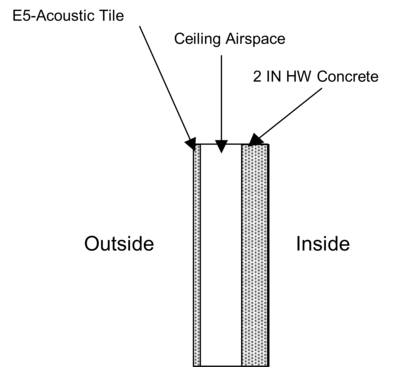
\includegraphics[width=0.9\textwidth, height=0.9\textheight, keepaspectratio=true]{media/image050.png}
\caption{Example Floor Construction illustration. \protect \label{fig:example-floor-construction-illustration.}}
\end{figure}

Window constructions are similarly built up from items in the Window Materials set using similar layers.. See Figure~\ref{fig:illustration-for-material-ordering-in}. Illustration for material ordering in windows, which shows the case where an interior shading layer such as a blind is present. The gap between the inside glass layer (layer \#3) and the interior shading layer is not entered. Similarly, for an exterior shading layer, the gap between the outside glass layer and the shading layer is not entered.

\begin{figure}[hbtp] % fig 25
\centering
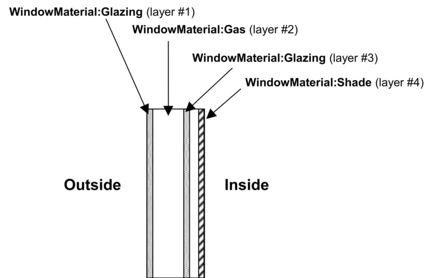
\includegraphics[width=0.9\textwidth, height=0.9\textheight, keepaspectratio=true]{media/image051.png}
\caption{Illustration for material ordering in windows. \protect \label{fig:illustration-for-material-ordering-in}}
\end{figure}

However, for a between-glass shading device the gaps on either side of the shading layer must be entered and they must have the same gas type. In addition, the gap widths with and without the between-glass shading layer must be consistent (see Figure~\ref{fig:window-construction-with-and-without-a}).

A maximum of four glass layers and one shading layer is allowed. A gas layer must always separate adjacent glass layers in a multi-pane glazing without a between-glass shading layer.

\begin{figure}[hbtp] % fig 26
\centering
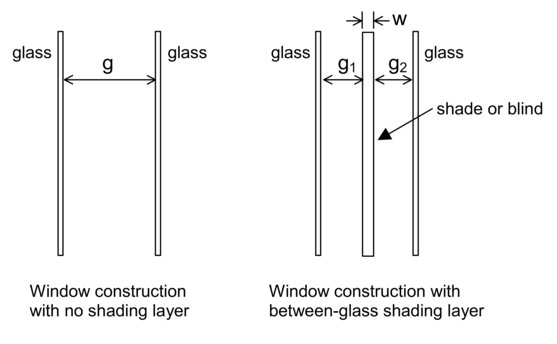
\includegraphics[width=0.9\textwidth, height=0.9\textheight, keepaspectratio=true]{media/image052.png}
  \caption{Window construction with and without a between-glass shading layer. Shown are gap widths \(g\), \(g_1\) and \(g_2\), and shading layer width, \(w\). An error will result if \(g_1 + g_2 +w\) is not equal to \(g\), where \(w\) is zero for a blind and greater than zero for a shade. \protect \label{fig:window-construction-with-and-without-a}}
\end{figure}

Outside and inside air film resistances are never given as part of a construction definitions since they are calculated during the EnergyPlus simulation. Note also that constructions are assumed to be one-dimensional in a direction perpendicular to the surface.

\subsubsection{Inputs}\label{inputs-34-000}

\paragraph{Field: Name}\label{field-name-28-001}

This field is a user specified name that will be used as a reference by other input syntax. For example, a heat transfer surface (ref: Building Surfaces) requires a construction name to define what the make-up of the wall is. This name must be identical to one of the Construction definitions in the input data file.

\paragraph{Field: Outside Layer}\label{field-outside-layer}

Each construction must have at least one layer. This field defines the material name associated with the layer on the outside of the construction---outside referring to the side that is not exposed to the zone but rather the opposite side environment, whether this is the outdoor environment or another zone. Material layers are defined based on their thermal properties elsewhere in the input file (ref: Material and Material Properties and Materials for Glass Windows and Doors). As noted above, the outside layer should NOT be a film coefficient since EnergyPlus will calculate outside convection and radiation heat transfer more precisely.

\paragraph{Field(s) 2-10: Layers}\label{fields-2-10-layers}

The next fields are optional and the number of them showing up in a particular Construction definition depends solely on the number of material layers present in that construction. The data expected is identical to the outside layer field (see previous field description). The order of the remaining layers is important and should be listed in order of occurrence from the one just inside the outside layer until the inside layer is reached. As noted above, the inside layer should NOT be a film coefficient since EnergyPlus will calculate inside convection and radiation heat transfer more precisely.

IDF Example (floor construction):

\begin{lstlisting}

Construction, FLOOR38,  ! Material layer names follow:
        E5 - ACOUSTIC TILE,
        E4 - CEILING AIRSPACE,
        C12 - 2 IN HW CONCRETE;
\end{lstlisting}

IDF Example (window construction, no shade):

\begin{lstlisting}

Construction, DOUBLE PANE WINDOW,  !- Material layer names follow:
        GLASS - CLEAR SHEET 1 / 8 IN,
        WinAirB1 - AIRSPACE RESISTANCE,
        GLASS - CLEAR SHEET 1 / 8 IN;
\end{lstlisting}

IDF Example (window construction, with interior shade):

\begin{lstlisting}

Construction, DOUBLE PANE WITH ROLL SHADE,  !- Material layer names follow:
        GLASS - CLEAR SHEET 1 / 8 IN,
        WinAirB1 - AIRSPACE RESISTANCE,
        GLASS - CLEAR SHEET 1 / 8 IN,
        ROLL SHADE - LIGHT
\end{lstlisting}

\subsection{Constructions - Modeling Underground Walls and Ground Floors Defined with C and F Factors for Building Energy Code Compliance}\label{constructions---modeling-underground-walls-and-ground-floors-defined-with-c-and-f-factors-for-building-energy-code-compliance}

Building energy code and standards like ASHRAE 90.1, 90.2 and California Title 24 require the underground wall constructions and slabs-on-grade or underground floors not to exceed certain maximum values of C-factor and F-factor, which do not specify detailed layer-by-layer materials for the constructions.

A simplified approach is introduced to create equivalent constructions and model the ground heat transfer through underground walls and ground floors for the building energy code compliance calculations. The approach is to create constructions based on the user defined C or F factor with two layers: one concrete layer (0.15 m thick) with thermal mass, and one fictitious insulation layer with no thermal mass. Three new objects were created for such purpose: \textbf{\hyperref[constructioncfactorundergroundwall]{Construction:CfactorUndergroundWall}}, \textbf{\hyperref[constructionffactorgroundfloor]{Construction:FfactorGroundFloor}}, and \textbf{\hyperref[sitegroundtemperaturefcfactormethod]{Site:GroundTemperature:FCfactorMethod}}. Details of the approach are described in the Engineering Reference document. The wall and floor construction objects are described in this section; the ground temperature object is described with the other ground temperature objects.

When a underground wall or ground floor surface (\hyperref[buildingsurfacedetailed]{BuildingSurface:Detailed}, \hyperref[floordetailed]{Floor:Detailed}, and \hyperref[walldetailed]{Wall:Detailed}) references one of the two construction objects, its field `Outside Boundary Condition' needs to be set to GroundFCfactorMethod. For simple (rectangular) wall and floor objects, the outside boundary condition is inferred from the construction type.

The \hyperref[sitegroundtemperaturefcfactormethod]{Site:GroundTemperature:FCfactorMethod} is described in the section for ground temperatures, the following section describes the two new construction objects.

\subsection{Construction:CfactorUndergroundWall}\label{constructioncfactorundergroundwall}

This input object differs from the usual wall construction object in that it describes an entire construction rather than individual layers. This object is used when only the wall height (depth to the ground) and the C-factor are available.~ This object accesses a model that creates an equivalent layer-by-layer construction for the underground wall to approximate the heat transfer through the wall considering the thermal mass of the earth soil.

This object is referenced by underground wall surfaces with their fields `Outside Boundary Condition' set to GroundFCfactorMethod.

\subsubsection{Inputs}\label{inputs-36}

\paragraph{Field: Name}\label{field-name-29-000}

The name of the underground wall construction.

\paragraph{Field: C-Factor}\label{field-c-factor}

C-Factor is the time rate of steady-state heat flow through unit area of the construction, induced by a unit temperature difference between the body surfaces. The C-Factor unit is W/m\(^{2}\)·K. The C-factor does not include soil or air films. ASHRAE Standard 90.1 and California Title 24 specify maximum C-factors for underground walls depending on space types and climate zones.

\paragraph{Field: Height}\label{field-height}

This field describes the height of the underground wall, i.e.~the depth to the ground surface. The unit is meters.

IDF Example:

\begin{lstlisting}

Construction:CfactorUndergroundWall,
      CfactorUGWall,
      0.436,           ! C-factor (W/m2K), does not include soil or air films
      4.57;            ! Height (m)


    BuildingSurface:Detailed,
      Zn001:Wall001,           !- Name
      Wall,                    !- Surface Type
      CfactorUGWall,           !- Construction Name
      ZONE ONE,                !- Zone Name
      GroundFCfactorMethod,    !- Outside Boundary Condition
      ,                        !- Outside Boundary Condition Object
      NoSun,                   !- Sun Exposure
      NoWind,                  !- Wind Exposure
      0.0,                     !- View Factor to Ground
      4,                       !- Number of Vertices
      0.0,0.0,4.572,           !- X,Y,Z = = > Vertex 1
      0.0,0.0,0.0,             !- X,Y,Z = = > Vertex 2
      15.24,0.0,0.0,           !- X,Y,Z = = > Vertex 3
      15.24,0.0,4.572;         !- X,Y,Z = = > Vertex 4
\end{lstlisting}

\subsection{Construction:FfactorGroundFloor}\label{constructionffactorgroundfloor}

This input object differs from the usual ground floor construction object in that it describes an entire construction rather than individual layers. This object is used when only the floor area, exposed perimeter, and the F-factor are available.~ This object accesses a model that creates an equivalent layer-by-layer construction for the slab-on-grade or underground floor to approximate the heat transfer through the floor considering the thermal mass of the earth soil.

This object is referenced by slab-on-grade or underground floor surfaces with their fields `Outside Boundary Condition' set to GroundFCfactorMethod.

\subsubsection{Inputs}\label{inputs-37}

\paragraph{Field: Name}\label{field-name-30-000}

The name of the ground floor construction.

\paragraph{Field: F-Factor}\label{field-f-factor}

F-Factor represents the heat transfer through the floor, induced by a unit temperature difference between the outside and inside air temperature, on the per linear length of the exposed perimeter of the floor. The unit for this input is W/m·K. ASHRAE Standard 90.1 and California Title 24 specify maximum F-factors for slab-on-grade or underground floors depending on space types and climate zones.

\paragraph{Field: Area}\label{field-area}

This field describes the area (in square meters) of the slab-on-grade or underground floor.

\paragraph{Field: PerimeterExposed}\label{field-perimeterexposed}

This field describes the exposed (direct contact with ambient air) perimeter (in meters) of the slab-on-grade or underground floor.

IDF Example:

\begin{lstlisting}

Construction:FfactorGroundFloor,
      slabconst,
      0.12,     !F-factor in W/m-K
      232.26,   !Area in m2
      61.0;     !Exposed perimeter in m


    BuildingSurface:Detailed,
      Zn001:Flr001,            !- Name
      Floor,                   !- Surface Type
      slabconst,               !- Construction Name, FLOOR
      ZONE ONE,                !- Zone Name
      GroundFCfactorMethod,    !- Outside Boundary Condition, Surface
      ,                        !- Outside Boundary Condition Object, Zn001:Flr001
      NoSun,                   !- Sun Exposure
      NoWind,                  !- Wind Exposure
      0,                       !- View Factor to Ground
      4,                       !- Number of Vertices
      15.24,0.0,0.0,           !- X,Y,Z = = > Vertex 1
      0.0,0.0,0.0,             !- X,Y,Z = = > Vertex 2
      0.0,15.240,0.0,          !- X,Y,Z = = > Vertex 3
      15.24,15.24,0.0;         !- X,Y,Z = = > Vertex 4
\end{lstlisting}

\subsection{ConstructionProperty:InternalHeatSource}\label{constructioninternalsource}

In some cases, such as radiant systems, a construction will actually have
resistance wires or hydronic tubing embedded within the construction. Heat is
then either added or removed from this building element to provide heating or
cooling to the zone in question. In the case of building-integrated
photovoltaics, the energy removed in the form of electricity will form a sink.
It is possible to enter such constructions into EnergyPlus with the syntax
described below. The internal source capability is available with both the
\textbf{ConductionTransferFunction} and \textbf{ConductionFiniteDifference}
solution algorithms. The only difference is that the two dimensional pipe
arrangements are not available to ConductionFiniteDifference. Those fields are
ignored in that implementation.

\subsubsection{Inputs}\label{inputs-38}

\paragraph{Field: Name}\label{field-name-31-000}

This field is a user specified name that will be used as a reference by other input syntax. For example, a heat transfer surface (ref: Building Surfaces) requires a construction name to define what the make-up of the wall is.

\paragraph{Field: Source Present After Layer Number}\label{field-source-present-after-layer-number}

This field is an integer that relates the location of the heat source or sink. The integer refers to the list of material layers that follow later in the syntax and determines the layer after which the source is present. If a source is embedded within a single homogenous layer (such as concrete), that layer should be split into two layers and the source added between them. For example, a value of ``2'' in this field tells EnergyPlus that the source is located between the second and third material layers listed later in the construction description (see layer fields below). This field must be between 1 and the number of material layers in the construction (maximum of 10 layers).

\paragraph{Field: Temperature Calculation Requested After Layer Number}\label{field-temperature-calculation-requested-after-layer-number}

The nature of this field is similar to the source interface parameter (see previous field) in that it is an integer, refers to the list of material layers that follow, and defines a location after the layer number identified by the user-defined number. In this case, the user is specifying the location for a separate temperature calculation rather than the location of the heat source/sink. This feature is intended to allow users to calculate a temperature within the construction. This might be important in a radiant cooling system where condensation could be a problem. This temperature calculation can assist users in making that determination in absence of a full heat and mass balance calculation. This field must be between 1 and the number of material layers in the construction (maximum of 10 layers).

It should also be noted that when using this construction in conjunction with a low temperature radiant system such as the \textbf{\hyperref[zonehvaclowtemperatureradiantvariableflow]{variable flow}}, \textbf{\hyperref[zonehvaclowtemperatureradiantconstantflow]{constant flow}}, or \textbf{\hyperref[zonehvaclowtemperatureradiantelectric]{electric}} radiant system that this parameter also defines the location for the temperature that is used with the Surface Interior Temperature control.  In other words, when using the Surface Interior Temperature control with a low temperature radiant system, the location for this temperature that is interior to the radiant surface is also defined in part by this input field.  Note that two fields below (\textbf{\hyperref[field-dimensions-for-the-ctf-calculation]{Dimensions for the CTF Calculation}} and \textbf{\hyperref[field-two-dimensional-temperature-calculation-position]{Two-Dimensional Temperature Calculation Position}}) will also have an impact on this location if the user elects to perform a 2-D solution for the surfaces using this construction.

\paragraph{Field: Dimensions for the CTF Calculation}\label{field-dimensions-for-the-ctf-calculation}

This field is also an integer and refers to the detail level of the calculation. A value of ``1'' states that the user is only interested in a one-dimensional calculation. This is appropriate for electric resistance heating and for hydronic heating (when boiler/hot water heater performance is not affected by return and supply water temperatures). A value of ``2'' will trigger a two-dimensional solution for this surface only. This may be necessary for hydronic radiant cooling situations since chiller performance is affected by the water temperatures provided.

A few things should be noted about requesting two-dimensional solutions. First, the calculation of the conduction transfer functions (CTF) is fairly intensive and will require a significant amount of computing time. Second, the solution regime is two-dimensional internally but it has a one-dimensional boundary condition imposed at the inside and outside surface (i.e., surface temperatures are still isothermal as if the surface was one-dimensional).

\paragraph{Field: Tube Spacing}\label{field-tube-spacing}

This field defines the distance between adjacent hydronic tubes spaced in the direction perpendicular to the main direction of heat transfer. The value for this parameter must be greater than or equal to 0.01m (or a tube spacing of 1 cm) and less than or equal to 1.0m (or a tube spacing of 1m). Note that this parameter is only used for two-dimensional solutions (see previous field) or when the user requests that the tube length for a hydronic radiant system ( \textbf{\hyperref[zonehvaclowtemperatureradiantvariableflow]{variable flow}} or  \textbf{\hyperref[zonehvaclowtemperatureradiantconstantflow]{constant flow}}) be autosized.  In the case of autosizing the tube length, this parameter is used along with the dimensions of the surface to approximate the tube length.

\paragraph{Field: Two-Dimensional Temperature Calculation Position}\label{field-two-dimensional-temperature-calculation-position}

This field only has a meaning when the user opts to have a two-dimensional solution in \textbf{\hyperref[field-dimensions-for-the-ctf-calculation]{Dimensions for the CTF Calculation}} above.  It is used in conjunction with the information in \textbf{\hyperref[field-temperature-calculation-requested-after-layer-number]{Temperature Calculation Requested After Layer Number}} above to specify a location for where the simulation will calculate a temperature at the interior of a surface.  The \textbf{\hyperref[field-temperature-calculation-requested-after-layer-number]{Temperature Calculation Requested After Layer Number}} field sets where the position is in the main direction of heat transfer.  This field determines the position of this point in the direction \textbf{perpendicular} to the main direction of heat transfer.  Note that this parameter is a dimensionless value that is allowed to range from 0.0 to 1.0.  A value of 0.0 is used for a position that is in line with the tubing in the construction.  A value of 1.0 is used for a position that is at the mid-point between adjacent tubes.  The user is also given the flexibility to select a point in between those two extremes.

It should also be noted that for values between 0.0 and 1.0 will not allow for
exact positioning of the point at which this temperature is calculated.
Instead, it will be used to calculate which node in the state space
representation will be used to calculate the temperature.  Currently,
EnergyPlus uses seven nodes in the direction perpendicular to the main
direction of heat transfer.  In this case, 0.0 represents the first node and
1.0 represents the seventh or last node in the perpendicular direction.  So,
this field will be used to determine which node in the direction perpendicular to
the main direction of heat transfer to use and there are five other nodes
(second, third, fourth, fifth, and sixth) that are possible locations.  For
example, if the user enters a value of 0.167, the second node will be used.
Likewise, if the user enters a value of 0.1, because this will be closest to
the second node, the second node will be used to calculate the internal
temperature.  For more information on two-dimensional heat transfer within
surfaces using ConstructionProperty:InternalHeatSource, please refer to the
EnergyPlus Engineering Reference.

\subsubsection{Outputs}\label{outputs-36-1}

\begin{itemize}
\item  Zone,Average,Surface Internal Source Location Temperature [C]
\item  Zone,Average,Surface Internal User Specified Location Temperature [C]
\item  Zone,Average,CondFD Internal Heat Source Power After Layer N [W]
\item  Zone,Average,CondFD Internal Heat Source Energy After Layer N [J]
\end{itemize}

\paragraph{Surface Internal Source Location Temperature {[}C{]}}\label{surface-internal-source-location-temperature-c}

This output is the temperature within the surface at the location of the source/sink.

\paragraph{Surface Internal User Specified Location Temperature {[}C{]}}\label{surface-internal-user—specified-location-temperature-c}

This output is the temperature within the surface at the location requested by the user.

\paragraph{CondFD Internal Heat Source Power After Layer}

This output is the heat power added after material layer N from the \hyperref[constructioninternalsource]{ConstructionProperty:InternalHeatSource} object. Only valid for the CondFD solution algorithm.

\paragraph{CondFD Internal Heat Source Energy After Layer}

This output is the heat energy added after material layer N from the \hyperref[constructioninternalsource]{ConstructionProperty:InternalHeatSource} object. Only valid for the CondFD solution algorithm.

\paragraph{CondFD EMS Heat Source Power After Layer}

This output is the heat power added after material layer N from the EMS heat flux actuator (Component type: ``CondFD Surface Material Layer''; Control type: ``Heat Flux''). Only valid for the CondFD solution algorithm.

\paragraph{CondFD EMS Heat Source Energy After Layer}

This output is the heat energy added after material layer N from the EMS heat flux actuator (Component type: ``CondFD Surface Material Layer''; Control type: ``Heat Flux''). Energy is aggregated on the electricity meter and is only valid for the CondFD solution algorithm.

\subsection{Construction:AirBoundary}\label{constructionairboundary}

Construction:AirBoundary indicates an open boundary between two zones. It may be used for base surfaces and fenestration surfaces.
When this construction type is used, the Outside Boundary Condition of the surface (or the base surface of a fenestration surface)
must be either \textit{Surface} or \textit{Zone}. A base surface with Construction:AirBoundary cannot hold any fenestration surfaces.

The two zones separated by this air boundary will be grouped together into a combined enclosure for solar distribution, daylighting, and radiant exchange (including distribution of radiant internal gains). If a given zone has an air boundary with more than one zone, then all of the connected zones will be grouped together. For example, if there is an air boundary between zones A and B, and another air boundary between zones B and C, all three zones (A, B, and C) will be grouped into a single enclosure. Normal default simplified view factors will apply unless detailed view factors are specified using \hyperref[zonepropertyuserviewfactorsbysurfacename]{ZoneProperty:UserViewFactors:BySurfaceName}.

\subsubsection{Inputs}\label{inputs-38-01}

\paragraph{Field: Name}\label{field-name-31-0001}

The name of the construction.

\paragraph{Field: Air Exchange Method}\label{field-air-exchange-method}

This field controls how the surface is modeled for radiant exchange calculations. There are two choices:

\begin{description}
  \item[None] There will be no air exchange modeled across this surface. Other objects, such as \hyperref[zonemixing]{ZoneMixing} and \hyperref[zonecrossmixing]{ZoneCrossMixing} or AirflowNetwork openings may be specified if desired.
  \item[SimpleMixing] For each pair of zones connected by Construction:AirBoundary, a pair of ZoneMixing objects will created automatically. These mixing objects may be automatically adjusted to balance HVAC system flows using the \hyperref[zoneairmassflowconservation]{ZoneAirMassFlowConservation} object.
\end{description}

\paragraph{Field: Simple Mixing Air Changes per Hour}\label{field-simple-mixing-air-changes-per-hour}

If the Air Exchange Method is \textit{SimpleMixing}* then this field specifies the air change rate [1/hr] using the volume of the smaller zone as the basis. The default is 0.5. If an AirflowNetwork simulation is active this field is ignored.

\paragraph{Field:Simple Mixing Schedule Name}\label{field-Simple-mixing-schedule-name}

If the Air Exchange Method is \textit{SimpleMixing} then this field specifies the schedule name for the air mixing across this boundary. If this field is blank, then the schedule defaults to always 1.0. If an AirflowNetwork simulation is active this field is ignored.

IDF Example:

\begin{lstlisting}
  Construction:AirBoundary,
    Air Wall,                !- Name
    SimpleMixing,            !- Air Exchange Method
    0.5,                     !- Simple Mixing Air Changes per Hour {1/hr}
    ;                        !- Simple Mixing Schedule Name
\end{lstlisting}

\subsection{Composite Wall Constructions}\label{composite-wall-constructions}

Standard constructions in EnergyPlus are built with the materials and layers described earlier. However, some configurations will not be adequately represented by using this approach. The Reference Data Set CompositeWallConstructions.idf contains constructions and associated materials for a set of \textbf{composite} walls. These are walls---such as stud walls---that have complicated heat-flow paths so that the conduction is two- or three-dimensional. Thermal bridges are one of the common terms for these complicated heat-flow paths; this dataset will help you represent these in EnergyPlus.

The materials here are \textbf{not} real materials but are ``equivalent'' materials obtained from finite-difference modeling. (The thickness, conductivity, density and specific heat values of the material layers for the different constructions have been taken from the ASHRAE report ``Modeling Two- and Three-Dimensional Heat Transfer through Composite Wall and Roof Assemblies in Hourly Energy Simulation Programs (1145-TRP),'' by Enermodal Engineering Limited, Oak Ridge National Laboratory, and the Polish Academy of Sciences, January 2001.). EnergyPlus will calculate conduction transfer functions using these materials. The heat transfer based on these conduction transfer functions will then be very close to what would be calculated with a two- or three-dimensional heat transfer calculation.

For stud walls, using these composite constructions will give more accurate heat flow than you would get by manually dividing the wall into a stud section and a non-stud section.

If your wall's exterior or interior roughness or thermal, solar or visible absorptances are different from those in the data set, you can make the appropriate changes to the first material (the outside layer) or the third material (the inside layer). \textbf{None of the other values should be changed.}

\begin{callout}
Complete description of the CompositeWallConstructions data set are found in the OutputDetailsAndExamples document.
\end{callout}

\subsection{Construction:ComplexFenestrationState}\label{constructioncomplexfenestrationstate}

This input object is used to describe the properties of a single state for complex fenestration.~ There are two parts to the input, 1) layer-by-layer physical description of fenestration system and 2) a set of matrices that describe overall system optical performance.~ Each layer also has associated with it two matrices that give the layer absorptance (for front and back incidence on the system).

The optical properties are given as a two-dimensional matrix describing the basis and four two-dimensional matrices of system bidirectional optical properties.

These input objects will generally be exported directly from the WINDOW program and it is expected that users usually will not develop the input themselves. However, this is an option for users who prefer to use a different method (e.g., Monte-Carlo ray-trace or measurement) of determining optical properties.

Multiple instances of this object are used to define the separate operating states of complex fenestration.~ For example, blinds could be deployed or redirected to create a new state, or electrochromic glazings could change transmittance.~ Each separate state defines the materials present and the overall optical performance.~ If the glazing system has only one state, then only one of these objects is needed.

If there is more than one complex fenestration state, it will be controlled using the EMS actuator called ``Surface'' with the control type ``Construction State'' and the EMS input object called \hyperref[energymanagementsystemconstructionindexvariable]{EnergyManagementSystem:ConstructionIndexVariable}.

Note that when using the Solar Distribution method of \textbf{FullInteriorAndExterior} or \textbf{FullInteriorAndExteriorWithReflections}, the Construction:ComplexFenestrationState windows are not suggested to be mix-used together with regular windows (windows constructed from ``actual'' materials descriptions, or simple layers) in the same zone, due to the limitations of the current models. When these two solar distribution methods are used, it is suggested using either all regular windows or all Complex Fenestration windows in the same zone, but not a mix of these two types of windows.

\subsubsection{Inputs}\label{inputs-39}

\paragraph{Field: Name}\label{field-name-32-000}

Unique name of this construction.~ Used to identify type of window in surface objects.

\paragraph{Field: Basis Type keyword}\label{field-basis-type-keyword}

Only value currently implemented is ``LBNLWINDOW''. More options may be added in the future.

\paragraph{Field: Basis Symmetry, keyword}\label{field-basis-symmetry-keyword}

Only value currently implemented is ``None''. More options will be added in the future.

\paragraph{Field: Thermal Parameters}\label{field-thermal-parameters}

This field gives the name of \hyperref[windowthermalmodelparams]{WindowThermalModel:Params} object used to keep common data necessary for thermal simulation.

\paragraph{Field: Basis Matrix Name}\label{field-basis-matrix-name}

This field gives the name of an 2 x N matrix object that defines the basis~ For a fenestration basis, N would be the number of theta (polar angle) values, the first of the two elements for each of the i = 1,..,N would be the theta value, and the second would be the number of phi (azimuthal angle) values that 360º is divided into for that theta.

\paragraph{Field: Solar Optical Complex Front Transmittance Matrix Name}\label{field-solar-optical-complex-front-transmittance-matrix-name}

This field contains the name of matrix object that describes the solar transmittance at different incident angles.~ This is from the outside toward the inside.

\paragraph{Field: Solar Optical Complex Back Reflectance Matrix Name}\label{field-solar-optical-complex-back-reflectance-matrix-name}

This field contains the name of matrix object that describes the solar back reflectance at different incident angles.~ This is from the inside toward the outside.

\paragraph{Field: Visible Optical Complex Front Transmittance Matrix Name}\label{field-visible-optical-complex-front-transmittance-matrix-name}

This field contains the name of matrix object that describes the visible transmittance at different incident angles.~ This is from the outside toward the inside.

\paragraph{Field: Visible Optical Complex Back Reflectance Matrix Name}\label{field-visible-optical-complex-back-reflectance-matrix-name}

This field contains the name of vector object that describes the visible back reflectance at different incident angles.~ This is from the inside toward the outside.

\paragraph{Field: Outside Layer \textless{}x = 1\textgreater{}}\label{field-outside-layer-x-1}

Each construction must have at least one layer. The layer order is from outside to inside, with the first layer being either \hyperref[windowmaterialglazing]{WindowMaterial:Glazing} or \hyperref[windowmaterialcomplexshade]{WindowMaterial:ComplexShade}. The next layer is a \hyperref[windowmaterialgap]{WindowMaterial:Gap} layer, and the following layers then alternate between \hyperref[windowmaterialglazing]{WindowMaterial:Glazing} or \hyperref[windowmaterialcomplexshade]{WindowMaterial:ComplexShade} and \hyperref[windowmaterialgap]{WindowMaterial:Gap}. The last layer cannot be \hyperref[windowmaterialgap]{WindowMaterial:Gap}.

\paragraph{Field: Outside Layer Directional Front Absorptance Matrix Name}\label{field-outside-layer-directional-front-absorptance-matrix-name}

Points to an Nbasis x 1 matrix object.

\paragraph{Field: Outside Layer Directional Back Absorptance Matrix Name}\label{field-outside-layer-directional-back-absorptance-matrix-name}

Points to an Nbasis x 1 matrix object.

\paragraph{Above 3 fields are optionally repeated for layers 2-10}\label{above-3-fields-are-optionally-repeated-for-layers-2-10}

These layers include gaps, which do not need to have matrix data specified.

An IDF example of complex fenestration with single layer:

\begin{lstlisting}

Construction:ComplexFenestrationState,       !- single layer example
    CFS_Glz_1,                 !- name
    LBNLWindow,                !- basis type
    None,                      !- basis symmetry type
    ThermParam_1,              !- window thermal model
    CFS_Glz_1_Basis,           !- basis matrix name
    CFS_Glz_1_TfSol,           !- Tfsol
    CFS_Glz_1_RbSol,           !- Rbsol
    CFS_Glz_1_Tfvis,           !- Tfvis
    CFS_Glz_1_Tbvis,           !- Tbvis
    Glass_102_Layer,           !- layer 1 name
    CFS_Glz_1_Layer_1_fAbs,    !- fAbs
    CFS_Glz_1_Layer_1_bAbs;    !- bAbs
\end{lstlisting}

An complex fenestration IDF example with double layer (first layer is shading device):

\begin{lstlisting}

Construction:ComplexFenestrationState,       !- double layer example
    CFS_Glz_59,                    !- name
    LBNLWindow,                    !- basis type
    None,                          !- basis symmetry type
    ThermParam_59,                 !- window thermal model
    CFS_Glz_59_Basis,              !- basis matrix name
    CFS_Glz_59_TfSol,              !- Tfsol
    CFS_Glz_59_RbSol,              !- Rbsol
    CFS_Glz_59_Tfvis,              !- Tfvis
    CFS_Glz_59_Tbvis,              !- Tbvis
    Shade_30001_Layer,             !- layer 1 name (shading device)
    CFS_Glz_59_Layer_1_fAbs,       !- fAbs
    CFS_Glz_59_Layer_1_bAbs,       !- bAbs
    Gap_1_Layer,                   !- layer 1 name
    ,                 !- absorptance matrices for gaps should be empty for now
    ,                              !- it is for future use
    Glass_3110_Layer,              !- layer 2 name
    CFS_Glz_59_Layer_3110_fAbs,    !- fAbs
    CFS_Glz_59_Layer_3110_bAbs;    !- bAbs
\end{lstlisting}

\subsection{WindowThermalModel:Params}\label{windowthermalmodelparams}

This input object is used with the \hyperref[constructioncomplexfenestrationstate]{Construction:ComplexFenestrationState}

\subsubsection{Inputs}\label{inputs-40}

\paragraph{Field: Name}\label{field-name-33-000}

Unique name of the window thermal model parameters.

\paragraph{Field: Calculation Standard}\label{field-calculation-standard}

The type of the calculation standard.~ The choices are:

\begin{itemize}
\item
  ISO15099
\item
  EN673Declared
\item
  EN673Design
\end{itemize}

The default is ISO15099.

\paragraph{Field: Thermal Model}\label{field-thermal-model}

The type of thermal model.~ The choices are:

\begin{itemize}
\item
  ISO15099
\item
  ScaledCavityWidth
\item
  ConvectiveScalarModel\_NoSDThickness
\item
  ConvectiveScalarModel\_withSDThickness
\end{itemize}

The default is ISO15099.

\paragraph{Field: SD Scalar}\label{field-sd-scalar}

Shading Device Scalar Factor. Only used for~ Thermal Model = Convective Scalar Model.~ Factor of venetian shading device layer contribution to convection. Real value between 0 (where the shading device contribution to convection is neglected) and 1 (where the shading device treated as ``closed'' -- as if it is a glass layer with thermal properties of SD slat material). Default: 1.0

\paragraph{Field: Deflection Model}\label{field-deflection-model}

The type of deflection model used to model deflection in windows and glass.~ The choices are:

\begin{itemize}
\item
  NoDeflection
\item
  TemperatureAndPressureInput
\item
  MeasuredDeflection
\end{itemize}

The default is NoDeflection.

\paragraph{Field: Vacuum Pressure Limit}\label{field-vacuum-pressure-limit}

The pressure (Pa) which will be considered to be the limit for vacuum glazing pressure.~ All pressures less than or equal to this pressure will be considered to be vacuum. Default: 13.238 Pa.

\paragraph{Field: Initial Temperature}\label{field-initial-temperature}

The temperature (\(^{o}\)C) of the gap in the time of fabrication.~ It is used only when WindowThermalModel:Params DeflectionModel = TemperatureAndPressureInput

\paragraph{Field: Initial Pressure}\label{field-initial-pressure}

The pressure (Pa) of the gap at the time of fabrication of the sealed glazing system unitIt is used only when WindowThermalModel:Params DeflectionModel = TemperatureAndPressureInput.

An IDF example for WindowThermalModel:Params (without deflection):

\begin{lstlisting}

WindowThermalModel:Params,
    ThermParam_59,                   !- name
    ISO15099,                        !- standard
    ISO15099,                        !- thermal model standard
    1.00,                            !- SD scalar
    NoDeflection;                    !- deflection model
\end{lstlisting}

An IDF example for thermal parameters (with deflection):

\begin{lstlisting}

WindowThermalModel:Params,
    ThermParam_59,                   !- name
    ISO15099,                        !- standard
    ISO15099,                        !- thermal model standard
    1.00,                            !- SD scalar
    TemperatureAndPressureInput,     !- deflection model
    ,                                !- vacuum pressure limit
    21.00,                           !- temperature at time of fabrication
    10000.00;                        !- pressure at time of fabrication
\end{lstlisting}

An IDF example for WindowThermalModel:Params for modeling vacuum glazing

\begin{lstlisting}

WindowThermalModel:Params,
  ThermParam_1006,                                    !- name
  ISO15099,                                           !- standard
  ISO15099,                                           !- thermal model
  1.0000,                                             !- SDScalar
  NoDeflection,                                       !- deflection model
  13.238;                                             !- vacuum pressure limit
\end{lstlisting}

\subsection{Matrix:TwoDimension}\label{matrixtwodimension}

This is input object is only used with \hyperref[constructioncomplexfenestrationstate]{Construction:ComplexFenestrationState} object to enter a two-dimensional matrix of values.

It is used to define the Basis Matrix for BSDF input data, and is also used to define the actual BSDF matrices data for the complete fenestration definition as well as the individual layers of the system.

The data are entered in row-major order: all the elements of row 1, followed by all the elements of row 2, etc.~ The number of values to be entered depends on the number of rows and the number of columns.~ Blank fields are treated as having been set to zero.

See example IDF file ``CmplxGlz\_{}SmOff\_{}IntExtShading.idf'' for the definition of two complex shading layers with matrix data defined.

\subsubsection{Field: Name}\label{field-name-34-000}

Unique name of matrix input object.

\subsubsection{Field: Number of Rows}\label{field-number-of-rows}

This field is the number of rows in the matrix.

\subsubsection{Field: Number of Columns}\label{field-number-of-columns}

This field is the number of columns in the matrix

\subsubsection{\textless{} Field Set: Value \# N \textgreater{}}\label{field-set-value-n}

Repeat entering value exactly the same number of times as the number of rows times the number of columns.

\subsubsection{Field: Value \# 1}\label{field-value-1-000}

This is the value of the matrix at the first row and first column.

\subsubsection{Field: Value \#2}\label{field-value-2}

This is the value of the matrix at the first row and the second column.

An IDF example of matrix for defining BSDF basis:

\begin{lstlisting}

Matrix:TwoDimension,       !- matrix for basis definition
    CFS_Glz_1_Basis,         !- basis matrix name
    9,                       !- number of rows
    2,                       !- number of columns
    0.00000, 1.00000,
    10.00000, 8.00000,
    20.00000, 16.00000,
    30.00000, 20.00000,
    40.00000, 24.00000,
    50.00000, 24.00000,
    60.00000, 24.00000,
    70.00000, 16.00000,
    82.50000, 12.00000;
\end{lstlisting}

\subsection{Construction:WindowEquivalentLayer}\label{constructionwindowequivalentlayer}

This object defines the construction for equivalent layer window (ASHWAT) model. This window can model various mix of glazing and shading layers combination. Shadings are defined as an integral part of the construction. The construction is defined by listing the layers name starting with outside layer and work your way to the inside Layer. Up to six solid layers (glazing and shade) and up to five gaps, i.e., a total of up to 11 layers maximum are allowed in equivalent layer window object. The solid layer types allowed are: Glazing, Insect Screen, Roller Blinds, Venetian Blind, and Drape Fabrics. This window model requires optical data of the individual glazing and shading layers to calculate the effective optical properties of the composite fenestration construction. Venetian blinds in equivalent layer window model can be in a fixed slat angle or has the option to control the slat angle in order to maximize visibility, or maximize solar gains. An equivalent-layer concept can simulate wide range of multiple glazing and shading layers combination and provides unlimited flexibility to combine different types of shading layers in a fenestration. The equivalent-layer window model does not support daylighting control. For the gap layer object any one of the five different Gas types can be specified: AIR, ARGON, XENON, KRYPTON, or CUSTOM. This window object is referenced by fenestration surfaces. For details of the model description refer to Equivalent Layer Fenestration Model section in Engineering Reference. The various layer objects that can be referenced in Equivalent Layer window model are:

\begin{lstlisting}
WindowMaterial:Glass:EquivalentLayer
WindowMaterial:Shade:EquivalentLayer
WindowMaterial:Drape:EquivalentLayer
WindowMaterial:Blind:EquivalentLayer
WindowMaterial:Screen:EquivalentLayer
WindowMaterial:Gap:EquivalentLayer
\end{lstlisting}

\subsubsection{Inputs}\label{inputs-41}

\paragraph{Field: Name}\label{field-name-35}

This field is a user specified name that will be used as a reference by other input syntax. For example, a heat transfer surface (ref: Fenestration) requires a construction name to define what the make-up of the fenestration is. This name must be identical to one of the Window Construction Equivalent Layer definitions in the input data file.

\paragraph{Field: Outside Layer}\label{field-outside-layer-2}

Each equivalent layer window construction must have at least one layer. This field defines the material name associated with the layer on the outside of the construction---outside referring to the side that is exposed to the outdoor environment or another zone. Material layers for equivalent layer window model are defined based on their thermal properties elsewhere in the input file (ref: WindowEquivalentLayerMaterialNames)

\paragraph{Field: Layer 2 -- Layer11}\label{field-layer-2---layer11}

The next fields are optional and the number of them showing up in a particular equivalent layer window construction definition depends solely on the number of material layers present in that construction. The data expected is identical to the outside layer field (see previous field description). The order of the remaining layers is important and should be listed in order of occurrence from the one just inside the outside layer until the inside layer is reached. As noted above, the inside layer should NOT be a film coefficient since EnergyPlus will calculate inside convection and radiation heat transfer more precisely.

An IDF example for this object, is shown below:

\begin{lstlisting}

Construction:WindowEquivalentLayer,
    Six Solid Layers Window,   !- Name
    INSCRN,                    !- Outside Layer
    Air GAP Outdoor 12.7mm,    !- Layer 2
    GLZGRY,                    !- Layer 3
    Argon GAP Sealed 12.7mm,   !- Layer 4
    FEP,                       !- Layer 5
    Xenon GAP Sealed 12.7mm,   !- Layer 6
    LOF1436,                   !- Layer 7
    Krypton GAP Sealed 12.7mm, !- Layer 8
    GLZCLR,                    !- Layer 9
    Air GAP Indoor 12.7mm,     !- Layer 10
    ShadeTrns;                 !- Layer 11
\end{lstlisting}

\subsection{Construction:WindowDataFile}\label{constructionwindowdatafile}

The WINDOW program, which does a thermal and optical analysis of a window under different design conditions, writes a data file (``Window data file'') containing a description of the window that was analyzed. The Construction:WindowDataFile object allows a window to be read in from the WINDOW data file---see ``Importing Windows from WINDOW.'' For information on adding a shading device to the window see ``\hyperref[windowpropertyshadingcontrol]{WindowShadingControl}.''

\subsubsection{Inputs}\label{inputs-42}

\paragraph{Field: Name}\label{field-name-36}

This is the name of a window on the Window data file. An error will result if EnergyPlus cannot find a window of this name on the file, or if the file, shown in the next field, is not present. The location of the data file should be specified in the File Name field. For details on what is done with the data if a matching window is found on the file see ``Importing Windows from WINDOW.''

\paragraph{Field: File Name}\label{field-file-name-000}

This is the file name of the Window data file that contains the Window referenced in the previous field. The field may include a full path with file name, for precise results. The field must be \textless{}= 100 characters. The file name must not include commas or an exclamation point. A relative path or a simple file name should work with version 7.0 or later when using EP-Launch even though EP-Launch uses temporary directories as part of the execution of EnergyPlus. If using RunEPlus.bat to run EnergyPlus from the command line, a relative path or a simple file name may work if RunEPlus.bat is run from the folder that contains EnergyPlus.exe.

If this field is left blank, the file name is defaulted to Window5DataFile.dat.

Input Example

\begin{lstlisting}
Construction:WindowDataFile,
  DoubleClear;            !- Name of a Window on the Window Data File
  ! Note -- Window5DataFile.dat is presumed to be in the "run" folder where EnergyPlus.exe is

FenestrationSurface:Detailed,
  Zn001:Wall001:Win001, !- Name
  Window,               !- Class
  DoubleClear,          !- Construction Name
  Zn001:Wall001,        !- Base Surface Name, and Target (if applicable)
  0.5,                  !- View Factor to Ground
  ,                     !- Frame/Divider name
   1.0,                 !- Multiplier
  4,                    !- Number of vertices
  0.548, 0.0, 2.5000,   !- X,Y,Z of Vertices
  0.548, 0.0, 0.5000,
  5.548, 0.0, 0.5000,
  5.548, 0.0, 2.5000;
\end{lstlisting}

An example showing use of specific data file name and complete path location follows:

\begin{lstlisting}
Construction:WindowDataFile,
  DoubleClear,          !- Name of a Window on the Window Data File
  C:\EnergyPlusData\DataSets\MyWindow.dat;
\end{lstlisting}

\subsubsection{Outputs}\label{outputs-4-016}

An optional report (contained in \textbf{eplusout.eio}) gives calculational elements for the materials and constructions used in the input. These reports are explained fully in the Output Details and Examples document.
